%%%%%%%%%%%%%%%%%%%%%%%%%%%%%%%%%%%%%%%%%%%%%%%%%%
\documentclass[a4paper,12pt]{report}
% Add 'twoside' to the document class for two-sided
%%%%%%%%%%%%%%%%%%%%%%%%%%%%%%%%%%%%%%%%%%%%%%%%%%
% Our stuff to set chapters, page size etc
\usepackage{Setup/avlthesis}
% Our stuff to set math defs etc
\usepackage{Setup/avldefs}   
% My stuff to set very personal defs
\usepackage{Setup/mydefs}   
%%%%%%%%%%%%%%%%%%%%%%%%%%%%%%%%%%%%%%%%%%%%%%%%%%

%%%%%%%%%%%%%%%%%%%%%%%%%%%%%%%%%%%%%%%%%%%%%%%%%%
% Font
\usepackage{times}         
%%%%%%%%%%%%%%%%%%%%%%%%%%%%%%%%%%%%%%%%%%%%%%%%%%
% Size, ams 
\usepackage{amsmath,amsfonts}
\usepackage[pdftex]{color,graphicx}
\usepackage{Setup/algorithm,Setup/algorithmic}

% Parskip package
\usepackage{parskip}
%%%%%%%%%%%%%%%%%%%%%%%%%%%%%%%%%%%%%%%%%%%%%%%%%%
% Natbib Reference Package
\usepackage{natbib}
%%%%%%%%%%%%%%%%%%%%%%%%%%%%%%%%%%%%%%%%%%%%%%%%%%
% Sort citations alphabetically
\usepackage{Setup/citesort}
%%%%%%%%%%%%%%%%%%%%%%%%%%%%%%%%%%%%%%%%%%%%%%%%%%
% Allow multirow tables
\usepackage{multirow}
%%%%%%%%%%%%%%%%%%%%%%%%%%%%%%%%%%%%%%%%%%%%%%%%%%
% Allow subfigures
\usepackage{subfigure}
%%%%%%%%%%%%%%%%%%%%%%%%%%%%%%%%%%%%%%%%%%%%%%%%%%
% landscape pages
\usepackage{lscape}
%%%%%%%%%%%%%%%%%%%%%%%%%%%%%%%%%%%%%%%%%%%%%%%%%%
% float package
\usepackage{float}
\floatstyle{ruled}
% \restylefloat{figure}
\restylefloat{table}
%%%%%%%%%%%%%%%%%%%%%%%%%%%%%%%%%%%%%%%%%%%%%%%%%%
%%%%%%%%%%%%%%%%%%%%%%%%%%%%%%%%%%%%%%%%%%%%%%%%%%
% Graphics
%%%%%%%%%%%%%%%%%%%%%%%%%%%%%%%%%%%%%%%%%%%%%%%%%%
% Define these
\def\xtitle{Myocardial Microstructure and its Role in Propagation Dynamics}
\def\xauthor{Matthew Gibb}
\def\xcollege{Lincoln College}
\def\xterm{Hilary Term, 2012}
\def\xkeywords{microstructure fibres sheets cardiac electrophysiology myocardium}
\def\xsubject{a subject}

%%%%%%%%%%%%%%%%%%%%%%%%%%%%%%%%%%%%%%%%%%%%%%%%%%
% Hyperref package (generates a hyperlinked table 
% of contents), and sets the pdf info from the title 
\usepackage[pdftex,colorlinks=true,linkcolor=black,citecolor=black,filecolor=black,urlcolor=black,pdftitle={\xtitle},pdfauthor={\xauthor},pdfkeywords={\xkeywords},pdfsubject={\xsubject}]{hyperref}
%%%%%%%%%%%%%%%%%%%%%%%%%%%%%%%%%%%%%%%%%%%%%%%%%%
\usepackage{rotfloat}
% multiple comma-delimited references in a \ref command
\usepackage{cleveref}
\setcounter{tocdepth}{1}
\begin{document}

\pagestyle{empty}
\setcounter{page}{1}
\pagenumbering{roman}

\def\localpath{ThesisFrontmatter}
% no need to alter ThesisFrontmatter/title.tex
\begin{titlepage}
\begin{center}
\vspace*{1.0cm}
\Huge
{\bf \xtitle}\\
\vspace*{2.5cm}
{\Large \bf
\xauthor\\
\xcollege\\
}
\vspace*{2.5cm}
\centerline{

\includegraphics[width=30mm]{ThesisFrontmatter/ps/crest}
}
\vspace*{1.5cm}
\normalsize
Computational Biology Research Group\\
Department of Computer Science\\
University of Oxford\\

[0.5cm]
{\bf \xterm}\\

\vspace{2cm}
This thesis is submitted to the Department of Computer Science,
University of Oxford, for the degree of Doctor of Philosophy. This
thesis is entirely my own work, and, except where otherwise indicated,
describes my own research.

\end{center}
\end{titlepage}


\sglspace
% edit the words in ThesisFrontmatter/abstract.tex
{
\Large
\noindent\makebox[3in][l]{\xauthor}\hfill\makebox[3in][r]{Doctor of
Philosophy} \vskip 1pt
\makebox[3in][l]{\xcollege}\hfill\makebox[3in][r]{\xterm}
}

\vskip 1cm

{
\LARGE \bf
\begin{center}
{\xtitle}
\end{center}
}

{
\large\bf
\begin{center}
Abstract
\end{center}
}

\setlength{\baselineskip}{16truept}
FROM TRANSFER THESIS:

Computational modelling and simulation, in close interaction with experiments, has provided invaluable insight into the biochemical, mechanical and electrophysiological function and dysfunction of the heart. However, limitations in imaging techniques and computing resources have precluded the analysis of tissue architecture near the cellular scale and the effect of this architecture on cardiac function.

It is the wider aim of this thesis to develop a framework to investigate the role of microstructure in cardiac propagation dynamics and arrhythmogenesis. An initial modelling study elucidates the effect of blood vessels in sustaining arrhythmic episodes, and how the accurate modelling of fibre direction in the vicinity of the vessels mitigates this detrimental mechanism. A mathematical model of fibre orientation in a simple geometry around blood vessels has been developed, based on information obtained from highly detailed histological and MRI datasets. A simulation regime was chosen, guided by the vasculature extracted from whole heart MRI images, to analyse ventricular wavefront propagation for different orientations and positions of blood vessels. Our results demonstrate not only that the presence of the blood vessels encourages curvature in the activation wavefront around the blood vessels, but further that vessels act to restrict and prolong phase singularities. When compared to a more simplistic implementation of fibre orientation, the model is shown to weaken wavefront curvature and reduce phase singularity anchoring. Having established the importance of microstructural detail in computational models, it seems expedient to generate accurate data in this regard. The first steps have been taken merging MRI and histological images, in order to present the first 3-D sub-cellular resolution images of cardiac tissue, segmented by tissue type. Models including this detail will be developed and simulation will yield a deeper understanding of the role of microstructure in arrhythmia.


\tableofcontents
\newpage
% edit the words in ThesisFrontmatter/acknowledgements.tex
%!TEX root = ../thesis.tex
\vspace*{20mm}
{
\Large\bf
\begin{center}
Acknowledgements
\end{center}
}

This thesis is the culmination of many years' work and would not have been possible without the help and support of many people. 

I would like to thank my supervisors Dr. Martin Bishop, Dr. Blanca Rodriguez and Dr. Vicente Grau. From the very beginning, Martin has been the strongest mentor and a role model for achievement. Martin has provided tutoring, practical expertise, professional advice, friendship, opportunity, life coaching, and help with pretty much everything, unrecognisably beyond what could be expected, and greatly to my betterment. Blanca has imparted the vision, structure, guidance and scientific context, in my writing, project planning and management that I utterly lacked upon undertaking this endeavour. Her focus on direction, outcome and purpose has translated into many other parts of my life and has transformed my effectiveness as a person. Both Martin's and Blanca's commitment of pastoral care has been humbling and in embarrasing contrast to the experience of many of my peers; without it I would never have completed this course. In all aspects of the imaging side of this project, from theoretical and methodological creation and development, through complex debugging, to analysis and evaluation of results, Vicente has imparted unerring clarity and insight. His patient (and often repeated!) explanation and direction has beaten seemingly insurmountable problems and failures. All my supervisors have shown Olympian patience, generosity, support and care. I am a profoundly wiser and more able person having worked with them, and I look forward to returning their kindness in the future.

The thesis presented is in no small part been made possible through discussions with members of the Computational Biology Group and beyond. In particular, I owe a great deal to Raf Bordas, who has on several occasions proffered game-changing advice on technology and computational techniques, and who's cumulative saving of my wasted time is measured in months. In the same way, I would also like to thank Joe Pitt-Francis, Pras Pathmanathan, Jon Cooper, Miguel Bernabeu, Kevin Burrage, Mikael Wallman, Robbie Shade and Gabriel Rosser for thrillingly geeky and productive exchanges.

As always, my Mum and Dad have been just amazing over the past few years, and always there for support when I needed it most. I would especially like to thank my Mum for being so consistently enthused about my research career, and I would especially like to thank my Dad for consistently hiding his abject and heart-broken disappointment in my career choice. I am very excited to take them and my sister on holidays, excursions and general treats from now on!

My research was funded by the EPSRC, through the Systems Biology Doctoral Training Centre. I was given a solid educational foundation in research techniques by the DTC, and made great friends there, discussions with many of whom have contributed to this thesis.

\newpage
% edit the words in ThesisFrontmatter/notation.tex
\vspace*{20mm}
{
\Large\bf
\begin{center}
Notation
\end{center}
}

\label{sec:Notation}
Throughout this thesis, the following conventions will be used for
typesetting mathematics unless otherwise indicated:
\begin{itemize}
\item{\bf 2D and general Vectors} are written in lower case bold: $\vec{a}$,
and a unit vector with a hat $\uvec{a}$. Where important to
differentiate between homogeneous and non-homogeneous vectors, the
latter will appear as
$\vec{\tilde{a}}$. Vectors are usually column vectors,
with elements specified by subscript index (eg.\
$\vec{x}=(x_1,x_2)\tra$). 
\item{\bf 3D Vectors}  are written in upper case bold: $\vec{A}$, with similar conventions to 2D vectors.
\item{\bf Matrices} are written in teletype: $\mat{A}$, and may have size indicated,
$\mat{A}_{3\times4}$. Where a matrix is square $\mat{A}_3$ is a $3\times 3$ matrix.
The entry in the $i$th row and $j$th column of the matrix is $\matd{A}{ij}$.
\item{\bf Tensors} are written in bold calligraphic:
$\tensorud{T}{jk}i$,$\tensoru{Q}{ijkl}$.
\item{\bf Quaternions} are written as
$\quat{a}$.
\item{\bf Projective Equality} (see Appendix) is denoted $\projeq$ ~.
\end{itemize}


\newpage
%%%%%%%%%%%%%%%%%%%%%%%%%%%%%%%%%%%%%%%%%%%%%%%%%%
\setcounter{page}{0}
\pagenumbering{arabic}
\pagestyle{thesisheadings}
%%%%%%%%%%%%%%%%%%%%%%%%%%%%%%%%%%%%%%%%%%%%%%%%%%
%
\def\localpath{Ch1}
\chapter{Introduction and Aims}
\dblspace
%!TEX root = ../thesis.tex
\chapter{Introduction and Aims}
\dblspace

\section{Motivation}
\label{sec:intro:motivation}
  Sudden cardiac death is the leading global cause of mortality, accounting for 39\% of all deaths in the UK. The economic cost due to the disease totals \pounds9 billion in this country alone. Ventricular fibrillation is a central aspect to many of these fatalities. However, many of the fundamental mechanisms underlying their onset, maintenance and termination are poorly understood, and effective therapies based on this understanding remain out of reach.
  
  Over the last century, experimental investigations into cardiac function during physiological and pathological conditions have allowed the general processes which produce arrhythmias to be characterised. In recent decades, experimental investigations have been complemented by computational and mathematical models which aim to simulate the biochemical, mechanical and electrophysiological function and dysfunction of the heart. The frequent validation of computational models with experimental data and use of modelling to guide new experimentation is bringing a new level to the understanding of cardiac function. This marriage of in silico and experimental investigation has made increasingly clear the important large-scale functional effects of small-scale anatomical structure. Very recently, several experimental techniques have provided high resolution data on both myocardial tissue structure and on healthy and pathological wavefront dynamics \cite{Burton2006,Plank2009,Bishop2010}. These advances notwithstanding, fine anatomical detail remains absent from the latest models and the effect of structure on wavefront dynamics has yet to be computationally investigated. This investigation will bring us closer to a profound and predictive understanding of arrhythmia and will eventually lead to more effective therapies to combat acute heart disease.
  
  MOTIVATE EACH CONTRIBUTION

\section{Aims}
READ RAF'S INTRO, MAKE WILD UNSUBSTANTIATED CLAIMS TO BE SUBSTANTIATED IN THE LIT REVIEW

\label{sec:intro:aims}
It is the wider aim of the thesis to develop a framework via which the role of microstructure in arrhythmia and electrophysiological pathology may be investigated, based upon information from the latest imaging techniques and leveraging state of the art high performance computing facilities. The chapter concludes by delineating the specific thesis aims and summarising the document structure. Guided by experimental findings, we aim to demonstrate the importance of blood vessels and myocardial anisotropy in electropropagation. We aim to construct accurate and detailed 3D images from high quality histology data at the tissue and whole-organ scale, and then to generate 3D tissue models based on this characterisation. To do so, new tools and algorithms need to be developed. Using these models, the way will be paved to quantify and classify the relative wavefront propagative changes due to epicardial vessels, myocardial fibres and tissue distributions. Applying both focussed and organ scale simulation, we aim to explore how anatomical detail feeds into the prevention, the onset, the stabilisation and the subsequent rectification of arrythmias.

\section{Exegesis}
\label{sec:intro:exegesis}
  The next chapter introduces some central underpinnings of the thesis, with an overview of cardiac anatomy and electrophysiology, and of modelling and imaging techniques. A thorough literature review follows in Chapter~3, showcasing the experimental and computational evidence that inhomogeneities in tissue direct electrical dynamics. It also outlines the state of the art in computational modelling and simulation, and reviews the attempts made so far in the imaging of cardiac tissue. Chapter~4 describes an initial study that reflects experimental findings, showing that epicardial arteries anchor phase singularities and prolong arrhythmic episodes, but that this anchoring is reduced by the smooth negotiation of myocardial fibres around the vessels. Chapter~5 presents the automated construction of a geometrically precise 3D histological tissue map, based on a set of coherent block face reference images. Chapter~6 leads directly from here, detailing a novel, robust and highly-performant registration method that improves greatly upon the results from Chapter~5. Chapter~7 concludes with a brief feasibility analysis of the extraction of microstructural features for simulation.
   % and a summary of the future directions stemming from the roots of progress presented in the previous chapters.



%%%%%%%%%%%%%%%%%%%%%%%%%%%%%%%%%%%%%%%%%%%%%%%%%%
%
\def\localpath{Ch2}
\chapter{Background Information}
% If you like chapter abstracts ...
\dblspace
\begin{quote}{\em %!TEX root = ../thesis.tex
In this chapter we review some central background to the coming chapters. A synopsis of cardiac anatomy is followed by a brief on the electrophysiolical structure and function of the heart on the cellular, tissue and organ scale. First we discuss the overall activation sequence during one full beat of the heart, along with the problems that can arise during this process. We go on to discuss the cellular machinery which transduces this cycle, and how tissue structure mediates its propagation. We explain a commonly implemented continuum-based model of wave propagation known as the bidomain model, and examine how this model can be simulated upon three-dimensional finite element meshes, constructed from morphologies extracted from medical images. We conclude the chapter with an overview of the imaging techniques that are used to reconstruct and align volumes from raw imaging data, and then to extract the tissue features and morphologies from the volumes.}\end{quote}

\section{Introduction}
\label{sec:review:introduction}
CONFIRMATION REPORT
Several short treatises follow the introduction: on cardiac anatomy; on electrophysiology; on methods in electrophysiological modelling; ending with some theory on imaging, registration and segmentation.
CONFIRMATION REPORT

\begin{figure*}[thbp]
\centerline{
\begin{tabular}{cc}
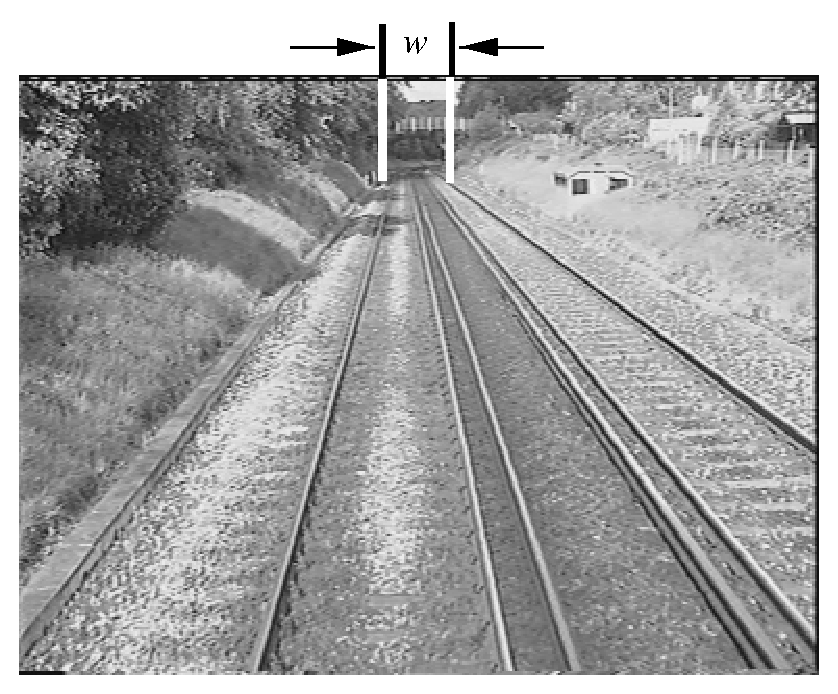
\includegraphics[width=65mm]{\localpath/Figs/calibim} &
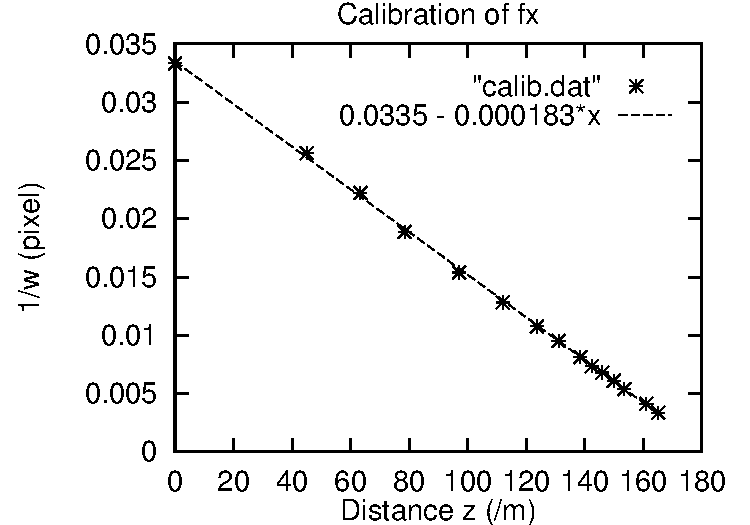
\includegraphics[width=85mm]{\localpath/Figs/calib} \\
(a) & (b)
\end{tabular}
}
\caption{\label{fig:review:calib}
(a) Image and 
(b) measured value of $1/w$ against $z$, and the fitted
straight line.
The slope 
is $1/f_xW = 1.83 \times 10^{-4}$pix$^{-1}$.m$^{-1}$
and the $z$-intercept is $D_o=183$m.
}
\hrule
\end{figure*}


\begin{equation}
\label{eq:review:rubbish}
a = \int_{0}^{1} x^{47} dx ~,
\end{equation}

\section{Algorithms in boxes}
The concensus is that it is best to put algorithms in boxes in
figures, as illustrated in Figure~\ref{fig:review:alg1}.

\begin{figure}
\centerline{\fbox{
\begin{minipage}{75mm}
\begin{algorithmic}
\REQUIRE $n \geq 0$
\ENSURE $y = x^n$
\STATE $y \Leftarrow 1$
\STATE $X \Leftarrow x$
\STATE $N \Leftarrow n$
\WHILE{$N \neq 0$}
\IF{$N$ is even}
\STATE $X \Leftarrow X \times X$
\STATE $N \Leftarrow N / 2$
\ELSE[$N$ is odd]
\STATE $y \Leftarrow y \times X$
\STATE $N \Leftarrow N - 1$
\ENDIF
\ENDWHILE
\end{algorithmic}
\end{minipage}
}}
\caption{\label{fig:review:alg1}
An algorithm in a box for finding the value of a number taken to a
non-negative power.}
\hrule
\end{figure}

\section{Cardiac Anatomy}
\section{Cardiac Electrophysiology}
\section{Electrophysiological Modelling}
\section{Segmentation}
\section{Registration}


%%%%%%%%%%%%%%%%%%%%%%%%%%%%%%%%%%%%%%%%%%%%%%%%%%
%
\def\localpath{Ch3}
\chapter{Literature Review}
% If you like chapter abstracts ...
\dblspace
\begin{quote}{\em %!TEX root = ../thesis.tex
  In this chapter we discuss previous work examining cardiac anatomy near the cellular scale and its influence on organ-scale function. We first motivate and direct our line of enquiry with experimental evidence, showing how microstructure has a profound effect on propagation dynamics and is central to future antitachycardia pacing treatments. Secondly, we detail the various sources of data available to us to fully characterise this structure, and weigh up their relative advantages and problems. Thirdly, we review the recent attempts to build coherent and geometrically accurate volumes from histology data. Finally, we explore the efforts made in the field to date to incorporate detailed anatomy into models for simulation, again demonstrating the important function of microstructure.

}\end{quote}
%!TEX root = ../thesis.tex
\chapter{Literature Review}
% If you like chapter abstracts ...
\dblspace
\begin{quote}{\em %!TEX root = ../thesis.tex
  In this chapter we discuss previous work examining cardiac anatomy near the cellular scale and its influence on organ-scale function. We first motivate and direct our line of enquiry with experimental evidence, showing how microstructure has a profound effect on propagation dynamics and is central to future antitachycardia pacing treatments. Secondly, we detail the various sources of data available to us to fully characterise this structure, and weigh up their relative advantages and problems. Thirdly, we review the recent attempts to build coherent and geometrically accurate volumes from histology data. Finally, we explore the efforts made in the field to date to incorporate detailed anatomy into models for simulation, again demonstrating the important function of microstructure.

}\end{quote}

\section{Evidence of the Role of Microstructure in Cardiac Electrical Dynamics} % (fold)
\label{sec:microstructure_has_profound_macroscopic_effects_on_propagation_dynamics}
  % Li et al. \cite{Li2010} observed sustained `locally synchronised ventricular fibrillation' in all of 6 dogs, the synchronicity of which they attribute largely to the Purkinje fibres.
  
  \subsection{Vessels, Trabeculae and Papillary Insertions} % (fold)
  \label{sub:vessels_trabeculae_and_papillary_insertions}
    \begin{figure}[htbp]
  		\centering
  		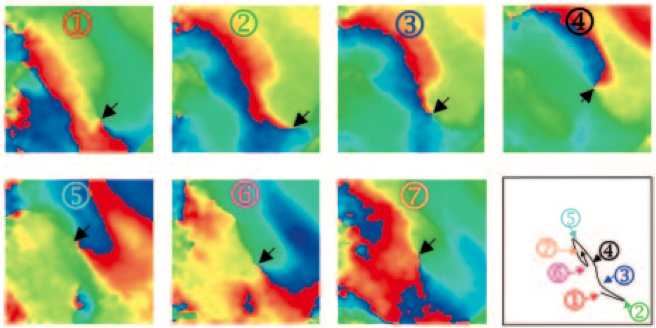
\includegraphics[width=1\textwidth]{Ch4/Figs/valderrabano}
      \caption{A meandering phase singularity from \cite{Valderrabano2003} along a rabbit epicardial artery. Seven sequential phase maps are shown with the trajectory of the singularity in the bottom right. The path is tightly restricted to the underlying artery.}
  		\label{fig:meandering}
  	\end{figure}
    
    It has been known for many years that structure at all scales mediates electrical propagation \cite{DeBakker2006}. Experimental studies demonstrate that microstructure, and specifically vascular and myocardial fibre structure, may be important in arrhythmia mechanisms. Phase singularities are areas of ambiguous activation state surrounded by tissue at all stages of the action potential, present during arrhythmia and fibrillation. They act as the organising centres of reentrant waves \cite{Gray1998}. Optical mapping studies show that phase singularities are restricted around and perpetuated by structural inhomogeneities. In one such study \cite{Valderrabano2003}, singularity clustering was noted in areas surrounding a sharp change or discontinuity in tissue type or fibre direction, such as epicardial vessels, ridges of endocardial trabeculae, and papillary muscle insertions; an example of such behaviour is shown in Figure~\ref{fig:meandering}. In a more recent rat tissue study \cite{Cysyk2008}, controlled placement of a 2-4mm hole (approximately the diameter of the largest vessels in a rat heart) in a homogenous monolayer of cells provides a defined site for wave pinning and excitation during field stimulation. A porcine electrical mapping study \cite{Qin2005} found that only anatomical heterogeneities such as those caused by sub-epicardial vessels were found to stabilise singularities and thus sustain fibrillation for up to 2 hours. Jalife et al. \cite{Jalife2000a} review evidence that ventricular fibrillation may be explained in terms of highly periodic three-dimensional rotors that activate the ventricles at exceedingly high frequency, and that these rotors can remain spatially stable around tissue features.

    During external electrical stimulation of cardiac tissue, secondary sources are induced at tissue inhomogeneities \cite{Sobie1997}, as distinct from the primary electrodes \cite{Roth1998}. In isolated rabbit right ventricular preparations \cite{Ripplinger2006} and in homogenous monolayers of neonatal rat cells \cite{Cysyk2008}, this effect has been exploited to stimulate tissue very near to an anchored phase singularity and unpin the associated spiral wave. In this way, much lower and less traumatic voltages can be applied to the heart to terminate arrhythmia and prevent the onset of fibrillation. These results were reflected in a theoretical study by Takagi et al. \cite{Takagi2004}, which shows that unpinning can be achieved with an electrical stimulus two orders of magnitude weaker than defibrillation energy.
    
    It is worth noting that these studies were limited. The 2D computational study by Takagi \cite{Takagi2004} was simplistic, considering a circular hole in a simplified geometry of isotropic tissue. None of the 2D mapping data obtained offers significant insight into wavefront dynamics below the epicardium or the role played by intramural blood vessels and deeper anatomical anchors in these dynamics. In the longer term, the placement of electrodes and timing of pulses during antiarrhythmic treatment cannot be optimised without accurate knowledge and understanding of reentrant wave propagation that confers real predictive power.
    
  % subsection vessels_trabeculae_and_papillary_insertions (end)

  \subsection{Tissue Type Distribution} % (fold)
  \label{sub:tissue_type_distribution}
    The distribution of ventricular cell and tissue types is also important in the initiation and maintenance of arrhythmia. For example, fibroblasts alter conduction velocity and refractoriness through several mechanisms. Traditionally, only cardiomyocyte decoupling was considered important, where fibroblasts act as passive insulating barriers, creating convoluted ‘zigzag’ conduction pathways and retarding propagation \cite{DeBakker2006,Spach2007}.
  
    Experimental studies have documented that functional gap junctions form between fibroblasts and myocytes \cite{Camelliti2004, Camelliti2005, Walker2007}. Gap junctions affect propagation in three main ways.  Firstly, the conductivity facilitated by the junctions enhances propagation, allowing fibroblasts to transduce activation between otherwise unconnected myocytes \cite{Gaudesius2003, Zlochiver2008}. Secondly and contrastingly, the junctions cause electrotonic loading; fibroblasts act as capacitors coupled to the myocytes, absorbing ionic currents and delaying myocyte activation \cite{Jacquemet2007, Xie2009}. Finally, the coupling elevates myocyte resting membrane potential, causing conduction velocity first to increase and then to decrease with increasing fibroblast concentration and/or gap junction conductance, until finally conduction failure occurs \cite{Miragoli2006, Xie2009}.
  
    Fibroblasts also modulate myocyte behaviour via the release of paracrine factors \cite{Pedrotty2009}. A recent 2D computational study by Xie et al. \cite{Xie2009} suggests that this mechanism adds to the range, complexity and significance of the interaction between the two cell types, whilst conceding that simulating laminar sheet structures using a 2D model may obscure potentially important 3D transfibre effects of the laminar clefts. It went on to say that a real 3D structure is needed for further study, ideally modelled on a realistic representation of 3D cell distribution and coupling.
  % subsection tissue_type_distribution (end)
  
  In short, there are multiple and dynamic interactions between mechano-electrical function and all scales of cardiac morphology, and these are of crucial relevance for normal beat-by-beat activity of the heart, as well as for pathogenesis and therapy. The study of these interactions requires accurate knowledge of cardiac three-dimensional structure, at multiple scales from sub-cellular levels to whole organ. In the next section, we discuss what has been achieved so far toward characterising this structure.
% section microstructure_has_profound_macroscopic_effects_on_propagation_dynamics (end)
  
  \subsection{Myocyte, Fibre and Sheet Orientation} % (fold)
  \label{sub:fibre_direction}
    It is clear that wave propagation is faster parallel to myocytes than perpendicular to them, but there exists great controversy over the three-dimensional arrangement of myocytes within the ventricular walls. Karlon et al. \cite{Karlon1998} automated the quantification of local myofibre disarray in mouse histological sections. Streeter et al. \cite{StreeterJr1969} observed that the myocardial fibres that constitute ventricular tissue are organised such that their angle from the horizontal plane varies transmurally. Much of the literature asserts that the ventricular myocytes are compartmentalized in the form of sheets, albeit that the extent of division, and interrelations, of the sheets is less well explained. Gilbert et al. \cite{Gilbert2007} unify seemingly conflicting features of many of the contemporary structural models, encompassing inter-subject structural variability and proposing the variability as the root source of debate on myocardial architecture. Others present the only muscular unit to be found within the myocardial walls as the cardiac myocyte itself, embedded within an aggregated matrix of fibrous tissue \cite{Anderson2009}. It is also unclear how microstructure reorganises under tissue's own mechanical deformation; ex-vivo DTMRI of hearts at various stages of systole has started to provide insight here \cite{Hales2012}.
  % subsection fibre_direction (end)
  
\section{Cardiac Tissue Can Accurately Be Characterised with High Resolution Images} % (fold)
\label{sec:cardiac_tissue_can_be_accurately_characterised_with_high_resolution_data}
  In this section, we first delineate the various modalities used to image the whole heart: MRI, DTMRI, Q-ball imaging, micro computed tomography, two-photon tissue cytometry and histology. We give an overview of the modelling work carried out with such data so far, and go on to discuss the problems with each modality. We outline how two modalities, either MRI and histology or more recently block face images and histology, can be combined to overcome the failings of each, and what progress has already been made in this regard.
  
  \subsection{MRI} % (fold)
  \label{sub:mri}
    Magnetic Resonance Imaging, or MRI, uses a powerful magnetic field to align the magnetisation of hydrogen nuclei in the imaged medium. Radio frequency fields are then applied in order to perturb the magnetic field, causing the aligned nuclei to process around the energy minimum of the static magnetic field. This procession creates a magnetic field of its own, which is detected by the scanner. Resolutions of up to 26.4 x 26.4 x 24.4$\mu$m have been resolved of rabbit hearts by Burton et al. \cite{Burton2006}, up to 21.5$\mu$m isotropic of rat hearts by Schneider et al. \cite{Schneider2004} and more recently, 25.4 x 25.4 x 12.5$\mu$m in fixed in vitro rat hearts. Recent developments have also shown the possibility of quantifying structure in the myocardium with para-cellular resolution, using contrast-enhanced MRI \cite{Gilbert2012}, in particular in the ex vivo setting. However, in contrast to histological approaches, this does not allow, at present, positive identification of cell size and type.
    
  % subsection mri (end)
  \subsection{DTMRI} % (fold)
  \label{sub:dtmri}
    Diffusion Tensor MRI (DTMRI or DTI) provides a measure for the rate of water diffusion in three perpendicular directions. Six or more diffusion weighted measurements are obtained from different orientations, at each voxel of a single DTI image. A symmetric tensor is then calculated from the data, with three perpendicular eigenvectors whose magnitudes represent the three principal diffusion rates in their respective directions. It has been shown that the three principal axes of diffusion in cardiac tissue are closely aligned with the direction along fibres, perpendicular to fibres within myocardial sheets, and perpendicular to both fibres and sheets \cite{Scollan1998}. The highest resolution obtained with this technique is 101.6$\mu$m isotropic resolution \cite{Bishop2009}.
  % subsection dtmri (end)
  
  \subsection{Q-Ball Imaging} % (fold)
  \label{sub:q_ball_imaging}
    Q-Ball imaging is an established high-angular resolution diffusion MRI technique, which uses MRI measurements taken at a large number of orientations to reconstruct the radially integrated displacement function in all directions at each voxel in the image: the Orientation Distribution Function (ODF). The ODF of a diffusion tensor can be understood as a unit sphere that has been scaled along each of the tensor's three eigenvectors by their associated eigenvalues, to form a spheroid. ODFs from Q-ball imaging, however, can take any form parameterised by orientation (for example, the two angles in spherical polar coordinates), constrained only by symmetry through the origin
    \begin{equation}
      F(\theta, \phi) = F(-\theta, \pi - \phi).
    \end{equation}
    This extra information can be used to discriminate between areas with a single, slowly varying fibre population, rapid fibre rotation and the co-existence of multiple populations of fibres with distinct orientations \cite{Dierckx2009}.
  
  % subsection q_ball_imaging (end)
  
  \subsection{Micro Computed Tomography} % (fold)
  \label{sub:micro_computed_tomography}
    Micro-computed tomography ($\mu$CT) is an emerging, non-invasive imaging modality that allows for non-destructive, high-resolution imaging of tissue \cite{Ragan2007,Deng2012}. It has been shown that $\mu$CT is well-suited for imaging of bones and calcified structures, but it provides low soft tissue contrast. Tissue such as heart muscle therefore requires pretreatment with specific stains or contrast agents. While $\mu$CT provides superior spatial resolution, compared to MRI (typically $<$ 10 $\mu$m \cite{Metscher2009,Stephenson2012}), it cannot resolve cellular composition of tissue.
  % subsection micro_computed_tomography (end)
  
  \subsection{Histology} % (fold)
  \label{sub:histology}
  In the process of histology, an ex-vivo heart can be perfused with various preparatory agents before being gradually infiltrated with wax, over the course of approximately 2 weeks. Once set, the hearts can be serially sectioned, and the resulting slices photographed under microscope. The slices may also be stained with various binding agents in order to visually identify the constituent tissue types. Burton et al. \cite{Burton2006} followed this procedure, obtaining a stack of histology images of resolution 1.1x1.1$\mu$m, with each slice of thickness 10$\mu$m. This  methodology provides the highest resolution and the clearest tissue type distinction of any imaging technique. One major drawback is clear: the positions of the slices within the final images are unrelated.
  
  Despite the rich data that these imaging modalities provide, each technology has its limitations. MRI does not impart any information about fibre direction, and little about tissue type. DTMRI only performs well in areas of uniform, slowly varying fibre direction. Furthermore, DTMRI data is often noisy along surface boundaries due to partial volume effects \cite{Alexander2001}. Dierckx et al. \cite{Dierckx2009} compared Q-Ball imaging with DTMRI, finding good agreement in areas of coherent myofibre direction where diffusion is approximately Gaussian, but large discrepancies where fibres crossed each other, or where there was a sharp change in fibre orientation. In these areas, the Gaussian assumption upon which DTMRI is founded breaks down, and the more general Q-ball approach, mapping an orientation distribution function, is more appropriate. Even so, the spatial resolution of any MRI technique does not currently approach the dimensions necessary to resolve a cardiac cell, of approximately 20 x 20 x 120$\mu$m for myocytes. Individual myocytes can be discerned from histological data, but the method is not only extremely time consuming, but inherently destructive and inapplicable for in vivo measurement. The preparation and fixing methods introduce several deformations from tissue shrinkage during processing, from mechanical forces during the slicing process, and from potentially inhomogeneous relaxation of sections before mounting onto microscope slides \cite{Burton2006}. Moreover, the challenge remains to coregister accurately the 2D slice images once they have been obtained.
  % subsection histology (end)
% section cardiac_tissue_can_be_accurately_characterised_with_high_resolution_data (end)

\section{Cellular-Resolution Tissue Volumes Can Be Reconstructed from Serial Histology} % (fold)
\label{sec:cellular_resolution_tissue_volumes_can_be_reconstructed_from_serial_histology}
  All 3D histology reconstruction methods are based on the acquisition of individual 2D histology images, whether from scans of the un-cut surface of the embedded tissue (so-called block face imaging) \cite{Sands2005,Sands2006,Rutherford2012}, or as sections \cite{Burton2006,Plank2009}. In the former case, 2D images are intrinsically registered, and so no alignment is necessary. In the latter case, images are brought into alignment either through registration amongst themselves, or to a coherent reference volume. It will be seen that the most recent methods draw together the advantages of both techniques.
  
  In 2002, Hooks et al. \cite{Hooks2002} sectioned a 0.8 x 0.8 x 3.7mm transmural segment of rat left ventricle and recorded an intrinsically registered volume image of cubic-1.56$\mu$m resolution using confocal microscopy. The resulting volume images were more detailed than any that had been seen before. Using similar techniques in 2012, Rutherford et al. \cite{Rutherford2012} produced a 5.6mm$^3$ volume surrounding a rat anterior left ventricular infarct, with cubic-1$\mu$m resolution. Unfortunately, this approach cannot resolve tissue sections much larger than the samples presented, and certainly not an entire heart.
  
  It is well documented in the literature that the asymmetrical curvature of an object cannot be recovered solely from a set of two dimensional sections. This issue is known as the `banana problem' \cite{Malandain2004,Lyon2012} or the `z-shift effect' \cite{Yushkevich2006}. Even so, substantial literature is published attempting to reconstruct volumes in the absence of a target geometry \cite{Chakravarty2006,Schmitt2006,Cifor2009,Cifor2011}.
  
  Registering slices to a reference volume circumvents the banana problem. Burton et al. \cite{Burton2006} paved the way for this conjunction by providing MRI rabbit cardiac images of 26.4 x 26.4 x 24.4$\mu$m voxel size with 1.1 x 1.1 x 10$\mu$m histology stacks of the same hearts. They exhibited an initial attempt at slice alignment, guided by the MRI data. First, the difference between adjacent slices was minimised by applying rigid 2D transformations to each slice. Next, they applied a partial differential equation-based approach, solved using a pyramidal and geometric multigrid scheme. While this approach is often used to correct distortion in histological images \cite{Keeling2005}, and is indeed capable of correcting major misalignments, it has an important drawback: by aligning adjacent slices they reduce inter-slice differences that might be fundamental in the description of heart anatomy.
  
  Since then, an automated pipeline has been developed, applying iterative 2D and 3D optimised deformations to register the stacks into the MRI geometry \cite{Mansoori2007}. Histology slices were stacked together into a volume and a rigid 3D transform was optimised to get an initial rough alignment with the MRI volume. Each histology slice was then rigidly registered in its 2D plane with the corresponding MRI slice. Iterations of 3D and 2D registrations are performed until the optimal rigid registration between the two volumes is obtained. In the last stage, non-rigid histology to MRI slice registration was performed using the Demons algorithm \cite{Thirion1995}. Histogram matching was applied as a preliminary step to ensure equal intensities between the two images, as required by the Demons algorithm. Despite some success with this procedure, the slices are ultimately registered to 2D MRI image that does not correspond to the histology, and the unconstrained non-rigid registration that was employed in the final stage led to unrealistic tissue distortions. These problems notwithstanding, the direct registration of histology to MRI is the best way to move towards global shape correctness if no other reference data is available, and is still a common procedure \cite{Alic2011,Osechinskiy2011,Kimm2012}.
  
  Some of the simplest reference-based registration methods rely on manual feature selection or expert hand-drawn atlases. Jagular et al. \cite{Jagalur2007} register thousands of mouse brain histological gene-expression images to expert atlases using automatically selected landmarks. An expert manual approach, whilst appropriate for a quick and approximate result from a small number of data, does not scale, is not repeatable and is prone to human bias.
  
  Block face images, taken from the surface of the fixated tissue volume before sectioning, provide an intrinsically coherent and precisely corresponding set of reference images. Although suitable for low-resolution alignment  \cite{Palm2010}, the reference images are very different in appearance to the histology, with a much lower spatial resolution, hindering accurate alignment. Even very small imperfections in the final mappings introduces jaggedness that renders volumetric microstructure almost imperceptible. Algorithms have been proposed to smooth out this noise through the more precise and reliable coregistration of adjacent slices, in both a sequential \cite{Yushkevich2006,Chakravarty2008} and simultaneous \cite{Feuerstein2011} manner. However, these methods are highly parameterised, often involving registrations at a number of scales, using only a subset of the image information available, and are often based on essentially subjective segmentations, rather than purely original images. Furthermore, only the nearest two neighbouring slices are used to dampen transformational noise, and therefore only the very highest frequency of noise can ever be reduced. Most recently, high-resolution reference images have been provided through the use of two-photon tomography and microtomy \cite{Huang2009,Ragan2012}.
  
  Yushkevich et al. attempt to correct for the banana effect in serially registered mouse \cite{Yushkevich2006} and human \cite{Adler2012} brain histological volumes. They first perform a rigid-body banana registration to approximate the dimensions of a full brain volume. Clearly, if a transform less constrained than rigid-body were used, then each slice would resemble the size and, depending on the constraint of the transform, the shape of the first reference slice. A prism-like volume would result, entirely unrelated to the true geometry of the organ. Yushkevich et al. obtain resampled 2D MRI images corresponding to each section via a rigid 3D registration of the MRI to the z-shifted histology. The volume produced from registering each section to these MRI images is jagged, and so the transformation parameters are Gaussian smoothed to recover some of the continuity of the serial volume. This approach goes a long way to combining the global fidelity of anchoring to a reference volume and the local smoothness of adjacent slice registration. Yet smoothness is limited by the level of success of the individual inter-slice registrations; any error or discontinuity in the serial volume will be transduced directly into the final result. In particular, any differential deformation of adjacent slices during sectioning, either affine or curved, could not be resolved by the rigid-body banana registration, and would manifest as disjoints through the tissue in the z-direction. Moreover, they themselves concede that the method entails a great deal of empirical parameterisation and manual intervention, from the slice segmentation, to the graph edge weighting of the adjacent slice selection, to the width of the Gaussian smoothing of the histology-to-MRI transform parameters.
  
  No mention of non-rigid transforms is made in the Yushkevich implementation. But conceivably, non-rigid interslice registrations could be integrated into the pipeline once the MRI correspondence planes had been established, initialised from the terminus of the rigid registrations. In this case, one would be faced with two disagreeable alternatives. On the one hand, a direct registration could be performed from each slice in the cylindrical, non-rigid banana volume to the reference volume. In this case, most of the slices would be so distant in size, shape and position from alignment with the reference slice as to preclude consistent, successful registration. A better solution would be to apply the Gaussian smoothing to the transforms from the non-rigid, prism-like banana volume to the reference volume. These transforms could be computed by composing the inverse of the transforms from the rigid banana volume to the non-rigid volume with the transforms from the rigid banana volume to the reference volume. Volumes would certainly be smoother than with the rigid smoothing, as adjacent non-rigid differences have been relaxed. Yet unnecessary errors and inaccuracies in alignment would still be present, as slices are only given one algorithmic run to align, and it is implausible that the freedoms inherent in the transform of choice exactly correspond to the distortions undergone by the tissue sections. Chapter~\ref{cha:diffusion_smoothing_registration_of_high_resolution_rat_histology} proposes a new general method to overcome these issues to produce highly coherent volumes.
  
  Chakravarty et al. \cite{Chakravarty2008} first rigidly align sections of whole mouse brain to an associated block face set, then apply a deformation field transformation to each slice, calculated as the mean of the parameters from defomation fields registering it to the two neighbouring slices. While this may go some way to reducing noise from the block face registrations, the maximum distance of information transfer is one slice, and so only the maximum distortion frequency will be damped.
  
  Techniques have been developed to combine monomodal adjacent slice and multimodal reference registrations simultaneously. Palm et al. \cite{Palm2008} expound a `weighted multi-image mutual information metric', optimising the sum of scaled contributions from both cost functions, and Feuerstein et al. \cite{Feuerstein2011} combine two potential energy functions in a Markov random field model to reconstruct a rat kidney. Not only do these methods require extraneous parameterisation and tuning, but in practice, the superposed cost function will form several distinct local minima; rather than reaching an averaged compromise between the reference images, the optimisation will arrive close to one preferred of several single-image minima, depending on the relative weightings and the transform initialisation.
  
  Atlases of both histology and MRI have been constructed by averaging histological volumes \cite{Li2009}, which were registered based on the approaches taken by \cite{Malandain2004,Yushkevich2006}. Having segmented mouse brain sections, their centres of mass were aligned and a rigid body registration was performed between adjacent slices. The banana effect was mitigated by a 3D registration to MRI, a slice-wise alignment of histological centres of mass to their MRI cross-section equivalent, and a final 3D non-rigid registration. Whilst perhaps appropriate for such low resolution data as presented, these methods are heuristic at best, and introduce several artificial sources of distortion.
  
  Finally, \cite{Arganda-Carreras2010} offer an interesting and robust approach to combining monomodal and multimodal alignments, using consistent b-spline-based elastic registrations. Multiple iterations of triple-wise registrations gradually share information in the z-direction and result in smoothing through a spectrum of scales. However, the choice of simultaneous registration leads to the same problem of multiple local minima faced by \cite{Palm2008,Feuerstein2011}.
% section cellular_resolution_tissue_volumes_can_be_reconstructed_from_serial_histology (end)

\section{The State of the Art in Modelling and Simulation Incorporates Microstructural Detail} % (fold)
\label{sec:the_state_of_the_art_in_microstructural_modelling_and_simulation_incorporates_microstructural_detail}
  Imaging techniques, image processing algorithms, mesh generation software \cite{Prassl2009} and simulation environments have been developed and woven together in recent years to model the electrical, and increasingly electromechanical, behaviour of the heart; the scope for detailed, rigorous and accurate modelling and simulation is widening. In this project, some of the most advanced toolkits available have been used, including ITK. Tarantula (www.meshing.at) is a proprietary program for generating tetrahedral meshes from volumetric data, used in several models of cardiac tissue \cite{Bernabeu2008,Bishop2006,Plank2009}. Two leading simulation environments, The Cardiac Arrhythmia Research Package (CARP, \cite{Vigmond2003}) and Cancer, Heart And Soft Tissue Environment (CHASTE, \cite{Pitt-Francis2008, Pitt-Francis2009, Pitt-Francis2009a}) have enabled large-scale electrophysiological simulations to be run on high performance computing facilities \cite{Bernabeu2008}.
  
  Computational models are increasingly being applied as a way to link spatio-temporal scales, complementing traditional “wet-lab” approaches and projecting between bench and bed-side \cite{Hunter2010,Kohl2010}. An abundance of three-dimensional anatomical models of the cardiac ventricles and atria have been constructed \cite{Eason1998,Kanai1995,Vetter2005,DeBakker2005,Atkinson2011,Baher2011,Bishop2009,Bishop2012,Bordas2010,Bordas2011,Deo2009,Keller2012,Moreno2011,Niederer2011,Okada2011,Potse2006,Romero2010,Seemann2006,TenTusscher2007,Trayanova2011,Vadakkumpadan2010,Zemzemi2011,Zhao2012,Plotkowiak2008}. Accurate microstructural information such as fibre direction is very difficult to obtain, and many of these models include it in a non-specific, rule-based way \cite{StreeterJr1969}. Some models of microstructure have been implemented with information acquired from high-resolution imaging modalities including DTMRI. The reader is referred to previously published reviews of specific areas of computational cardiac electrophysiology \cite{Rudy2006,Brennan2009,Clayton2010,Clayton2011,Greenstein2011,Trayanova2011,Carusi2012}. The simulations based upon all of these models have provided unprecedented insight into the relationship between cardiac structure and function.

  % Fiber architecture is usually incorporated into tissue models by extracting information from histological or diffusion tensor-MRI images using image processing algorithms or using a mathematical rule that relates fiber rotation at a particular location with distance to the surfaces of the ventricular wall (43, 51, 77, 103, 111).
    
  Hooks et al. \cite{Hooks2002} opened a new direction in detailed image-derived 3D cardiac modelling. They manually constructed a finite element mesh from a volume image of a transmural rat heart segment.  Discontinuous bidomain simulations demonstrated for the first time that the laminar organisation of cardiomyocytes into sheets determines unique electrical properties tangential and normal to the sheets. Furthermore, interlaminar clefts between layers of myocytes were seen to act as secondary sources of electrical activation when an external shock is applied. The results were experimentally corroborated in a later study by the same group \cite{Hooks2007}, where arrays of intramural plunge electrodes measured voltage after stimulation in live pigs. The hearts were then removed, treated, frozen and histologically sectioned. The model of the reconstructed histology formed the basis of the subsequent conductivity tensor estimations.
  
  In 2006, Potse et al. \cite{Potse2006} pioneered whole-heart simulations based on MRI data with a rule-based muscle fibre direction, in order to compare monodomain and bidomain ionic models. In bidomain models extended to include fibroblasts \cite{Sachse2009}, increased myocyte-fibroblast coupling and fibroblast-myocyte ratio reduced peak voltage and maximal upstroke velocity of myocytes as well as amplitudes and maximal downstroke velocity of extracellular potentials. The most up-to-date models are now including a wealth of geometrical and structural information derived from high resolution MRI and histology imaging datasets. Xie et al \cite{Xie2004} investigate the interaction between fixed heterogeneities and dynamical instabilities in fibrillation in a canine cardiac geometry with DTMRI-based fibre orientation. Bishop et al. \cite{Bishop2009} highlight the utility of histoanatomically detailed models for investigations of cardiac function, in particular for future patient-specific modelling. They compared simulations from two rabbit heart meshes derived from the same MRI data, with one including finer detail and structure, such as trabeculae and blood vessels. It is observed that trabeculae act as stimulation short cuts, and vessels act as virtual electrodes to damp external stimulation. In another study \cite{Bishop2009a}, they compare fibre directions obtained from DTMRI with those from a rule-based algorithm in rat, and found a close overall match between simulations based on the two models. Overall, the inclusion of anatomical detail, when compared to lower resolution models, alters simulated wave propagation both locally and globally.

  Including details such as blood vessels as well as accurately representing the fibre structure around and within them might be important in understanding the complex morphology of intramural wavefronts beneath the epicardial surface. Some \cite{Ding2001,Hyatt2003} have suggested how surface-recorded optical signals can provide information regarding the sub-surface wavefront propagation direction, although how well this technique relates to more complex anatomical models has been disputed \cite{Bishop2006}. The inclusion of extra anatomical detail, such as vessels and the complex fibre structure around them, may influence wavefront morphology as well as affecting the surface-recorded optical mapping signal.
  
  We have seen that computational modelling techniques can provide a unique window of inference into true 3D propagation. Hitherto however, those models have not included an accurate representation of myocardial fibre orientation, neither do they incorporate high-resolution tissue type mapping. Images of the quality necessary to resolve this detail have been made available, and it is now possible to integrate the information they provide into our modelling and simulation frameworks.
% section sec:the_state_of_the_art_in_microstructural_modelling_and_simulation_incorporates_microstructural_detail (end)

\section{Conclusion} % (fold)
\label{sec:conclusion}
  In summary, microstructure is central to certain mechanisms of arrhythmia, and elucidating the nature of its contribution may eventually aid the diagnosis and treatment of heart disease. Images of the quality required to resolve microstructure are now available. Coherent, full-colour, cellular-resolution, whole-organ, histological tissue volumes can be reconstructed, and microstructural properties can be extracted, using the latest imaging algorithms and techniques. However, these methods all have their own weaknesses. The results of simulations incorporating the newly resolved structure offer a path of insight into the mechanisms of arrhythmia.
% section conclusion (end)

d
%%%%%%%%%%%%%%%%%%%%%%%%%%%%%%%%%%%%%%%%%%%%%%%%%%
%
\def\localpath{Ch4}
\chapter{Computational and Mathematical Techniques}
% If you like chapter abstracts ...
\dblspace
\begin{quote}{\em %!TEX root = ../thesis.tex

This chapter contributes a quantitative demonstration that the definition of microstructure affects electrical simulation results. We generate both a simplistic and a histologically based model of fibre direction around blood vessels, and use the models to construct idealised cuboid sections of ventricular wall containing transmural and epicardial vessels. We conduct electrophysiological simulations and compare the histologically based and the simplistic models, in order to distinguish the effects of the vessel cavity with those of the surrounding fibres. We also examine the effect of bidomain vs. monodomain simulations. We show that the activation patterns around blood vessels are similar for bidomain and monodomain simulations. We conclude that inhomogeneities in cardiac tissue such as blood vessels can cause sharp wavefront curvature. We find that this curvature is less pronounced when fibre direction is modelled accurately around the vessels, as the wavefront is guided around the vessel by the curving fibres. Finally, we find that contrary to what we had hypothesised, negotiation of fibres around vessels actually diminishes vessel anchoring by funnelling the wavefront around the vessel, lessening its retarding and fragmenting effect.}\end{quote}

\section{Introduction}
\label{sec:review:introduction}
CONFIRMATION REPORT
The bulk of the theory and technologies underpinning the research is expounded here.
\section{Segmentation}
  The methods of threshold segmentation, fast marching filtering and threshold segmentation level set filtering are explained, along with their advantages over other segmentation methods. The segmentation pipeline is delineated. A plan for this section is complete, and the writing needs to be expanded.
\section{Registration}
  The motivations and ideas behind registration are briefly discussed, and the generic structure of a registration pipeline is given. The individual components of the pipeline are examined, and the strengths and weaknesses of specific algorithms and strategies are presented in each case. Masking and sampling are touched upon. This section is effectively complete.
\section{Modelling Cardiac Electrophysiology}
We discuss cell ionic models and anisotropic diffusion based on tissue structure. The ionic model section needs significant work, but the tissue structure section was included in the transfer thesis.
\section{Finite Element Methods}
  The mathematical basis for the bidomain and monodomain equations is treated, along with their solution on a finite element mesh. I have a very strong grasp on the mathematics in both cases; the bidomain and monodomain section was included with the transfer, and the finite element section must be written up.
CONFIRMATION REPORT




%%%%%%%%%%%%%%%%%%%%%%%%%%%%%%%%%%%%%%%%%%%%%%%%%%
%
\def\localpath{Ch5}
\chapter{Comparison of an Accurate and Simplified Fibre Model in an Idealised Geometry}
% If you like chapter abstracts ...
\dblspace
\begin{quote}{\em %!TEX root = ../thesis.tex
The automated registration of hundreds of histological slices to a set of references requires a great measure of experimentation, parameterisation and tuning. This chapter contributes the tools and methods to reconstruct sub-cellular resolution whole-organ histological volumes, based on coherent block face images and accurately faithful to the true geometry of the organ.

We develop an incremental pipeline for the particular application of an entire rat heart volume. We list a range of appropriate preprocessing steps and evaluate two methods of transform initialisation. We discuss which metrics and optimisation strategies prove most successful in this context. We outline the most important architectural patterns which lead to code quality and maintainability, and which facilitate rapid prototyping and feedback with limited and diverse computational resources. We develop diagnostic tools to gain deep quantitative insight into the evolution of the registration algorithm, and with the indispensible information gleaned from them, we illustrate a solid general approach to parameter tuning. We showcase the registered rat heart volume, to serve as an anatomical reference, to validate current anatomical models used in simulation, and to inform future experimental and computational technique.
}\end{quote}
%!TEX root = ../thesis.tex
\chapter{Coregistration of High Resolution Rat Histology} % (fold)
\label{cha:coregistration_of_high_resolution_rat_histology}
% If you like chapter abstracts ...
\dblspace
\begin{quote}{\em %!TEX root = ../thesis.tex
The automated registration of hundreds of histological slices to a set of references requires a great measure of experimentation, parameterisation and tuning. This chapter contributes the tools and methods to reconstruct sub-cellular resolution whole-organ histological volumes, based on coherent block face images and accurately faithful to the true geometry of the organ.

We develop an incremental pipeline for the particular application of an entire rat heart volume. We list a range of appropriate preprocessing steps and evaluate two methods of transform initialisation. We discuss which metrics and optimisation strategies prove most successful in this context. We outline the most important architectural patterns which lead to code quality and maintainability, and which facilitate rapid prototyping and feedback with limited and diverse computational resources. We develop diagnostic tools to gain deep quantitative insight into the evolution of the registration algorithm, and with the indispensible information gleaned from them, we illustrate a solid general approach to parameter tuning. We showcase the registered rat heart volume, to serve as an anatomical reference, to validate current anatomical models used in simulation, and to inform future experimental and computational technique.
}\end{quote}

\section{Aims} % (fold)
\label{sec:aims}

  Having shown in an idealised geometry that fibre direction could have a significant effect on propagation, the challenge is set to characterise cardiac tissue at sufficient detail to resolve both fibre direction and other microstructure. Cell type distribution, the shape of tissue boundaries, the Purkinje fibre network, sheet structure and vasculature all affect macroscopic wave propagation, and must therefore be incorporated into electrophysiological models.
	
  The aim of this chapter is to develop an automated pipeline to register high resolution rat cardiac datasets robustly and accurately, and generate for the first time coherent whole-organ subcellular resolution 3D cardiac histological images. One full rat heart dataset will be processed through the pipeline to provide registered volumes. These images will serve both as an authoritative anatomical reference, and as the basis for anatomically based models in simulation studies, laying the foundations for the investigation of the role of microstructure in propagation dynamics.
	
% section aims (end

\section{Methods} % (fold)
\label{sec:methods}
	The methods developed to fulfil the aims of this work form the main part of the chapter. First we discuss the experimental acquisition, curation and digital preparation of the images. We go on to cover the algorithms that calculate reasonable starting transformations and refine those transformations via iterative registration. An overview of the tools' architecture precedes the methods developed for diagnostics and parameter tuning.
	
  \subsection{Image Acquisition} % (fold)
  \label{sub:image_acquisition}
    Hearts were isolated from female rats and cannulated via the aorta to a Langendorff perfusion system, in a similar manner to that presented in \cite{Burton2006}. The hearts were then fixed and stabilised in agar, and 25.4 x 25.4 x 12.7$\mu$m MRI scans were performed. The hearts were immersed in increasing concentrations of alcohol, in order to dehydrate them before embedding them in black wax. The wax blocks were then serially sectioned at 10$\mu$m thickness using a microtome. An image of the top surface of the block -- referred to as a `block face image' from here on -- was taken with 25$\mu$m resolution after each slicing. Every 5th section was Trichrome stained, labelling connective tissue bluish-green, myocytes pinkish-red and nuclei blue-black. Each slice was relaxed and re-hydrated, before histology imaging was performed using a 5x objective with 1.1$\mu$m resolution, the resultant images being referred to as `histology images' from here on. Examples of the block face and slice images are displayed in Figures~\labelcref{fig:original_lores_images,fig:original_hires_images}, respectively.
		
		\begin{figure}[htbp]
		  \centering
		  \subfigure[][]{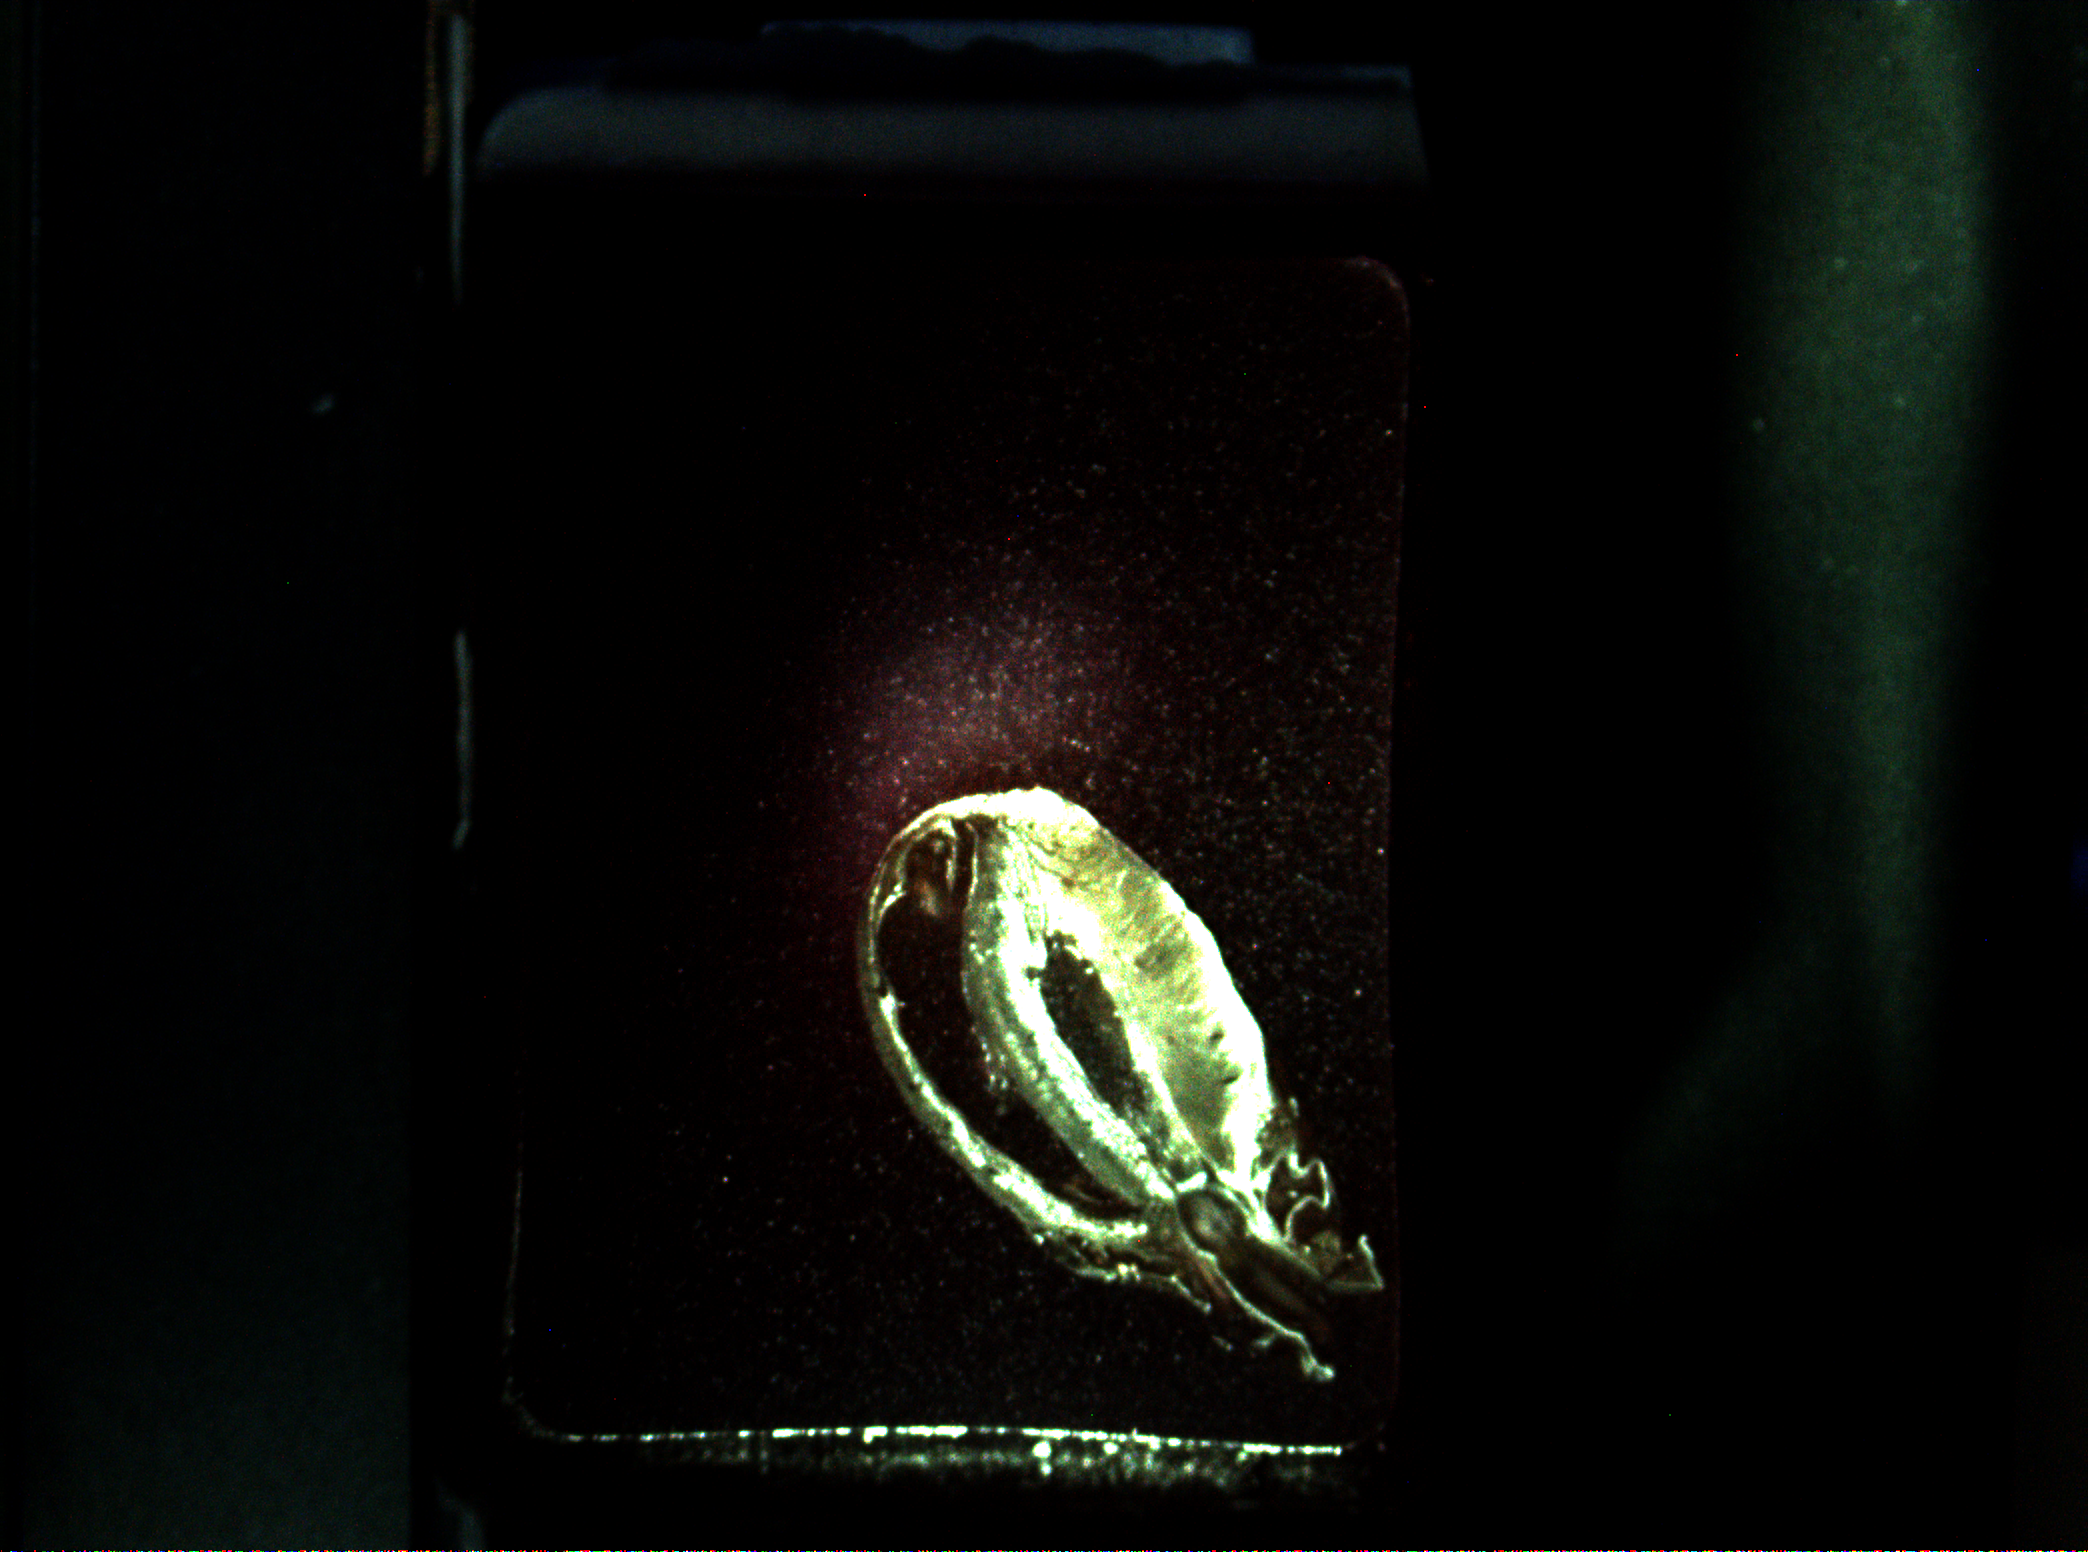
\includegraphics[width=0.8\pagewidth]{Ch5/Figs/LoRes_rgb_downsamples_1_0582}}
		  \subfigure[][]{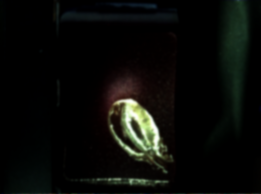
\includegraphics[width=0.8\pagewidth]{Ch5/Figs/LoRes_rgb_downsamples_8_0582}}
		  \caption{Block face images of slice 582 of Rat 28. The original image is shown in \textbf{(a)}, with \textbf{(b)} Gaussian smoothed and downsampled by a factor of 8 in each dimension.}
		  \label{fig:original_lores_images}
		\end{figure}
    
    \begin{figure}[htbp]
      \centering
      \subfigure[][]{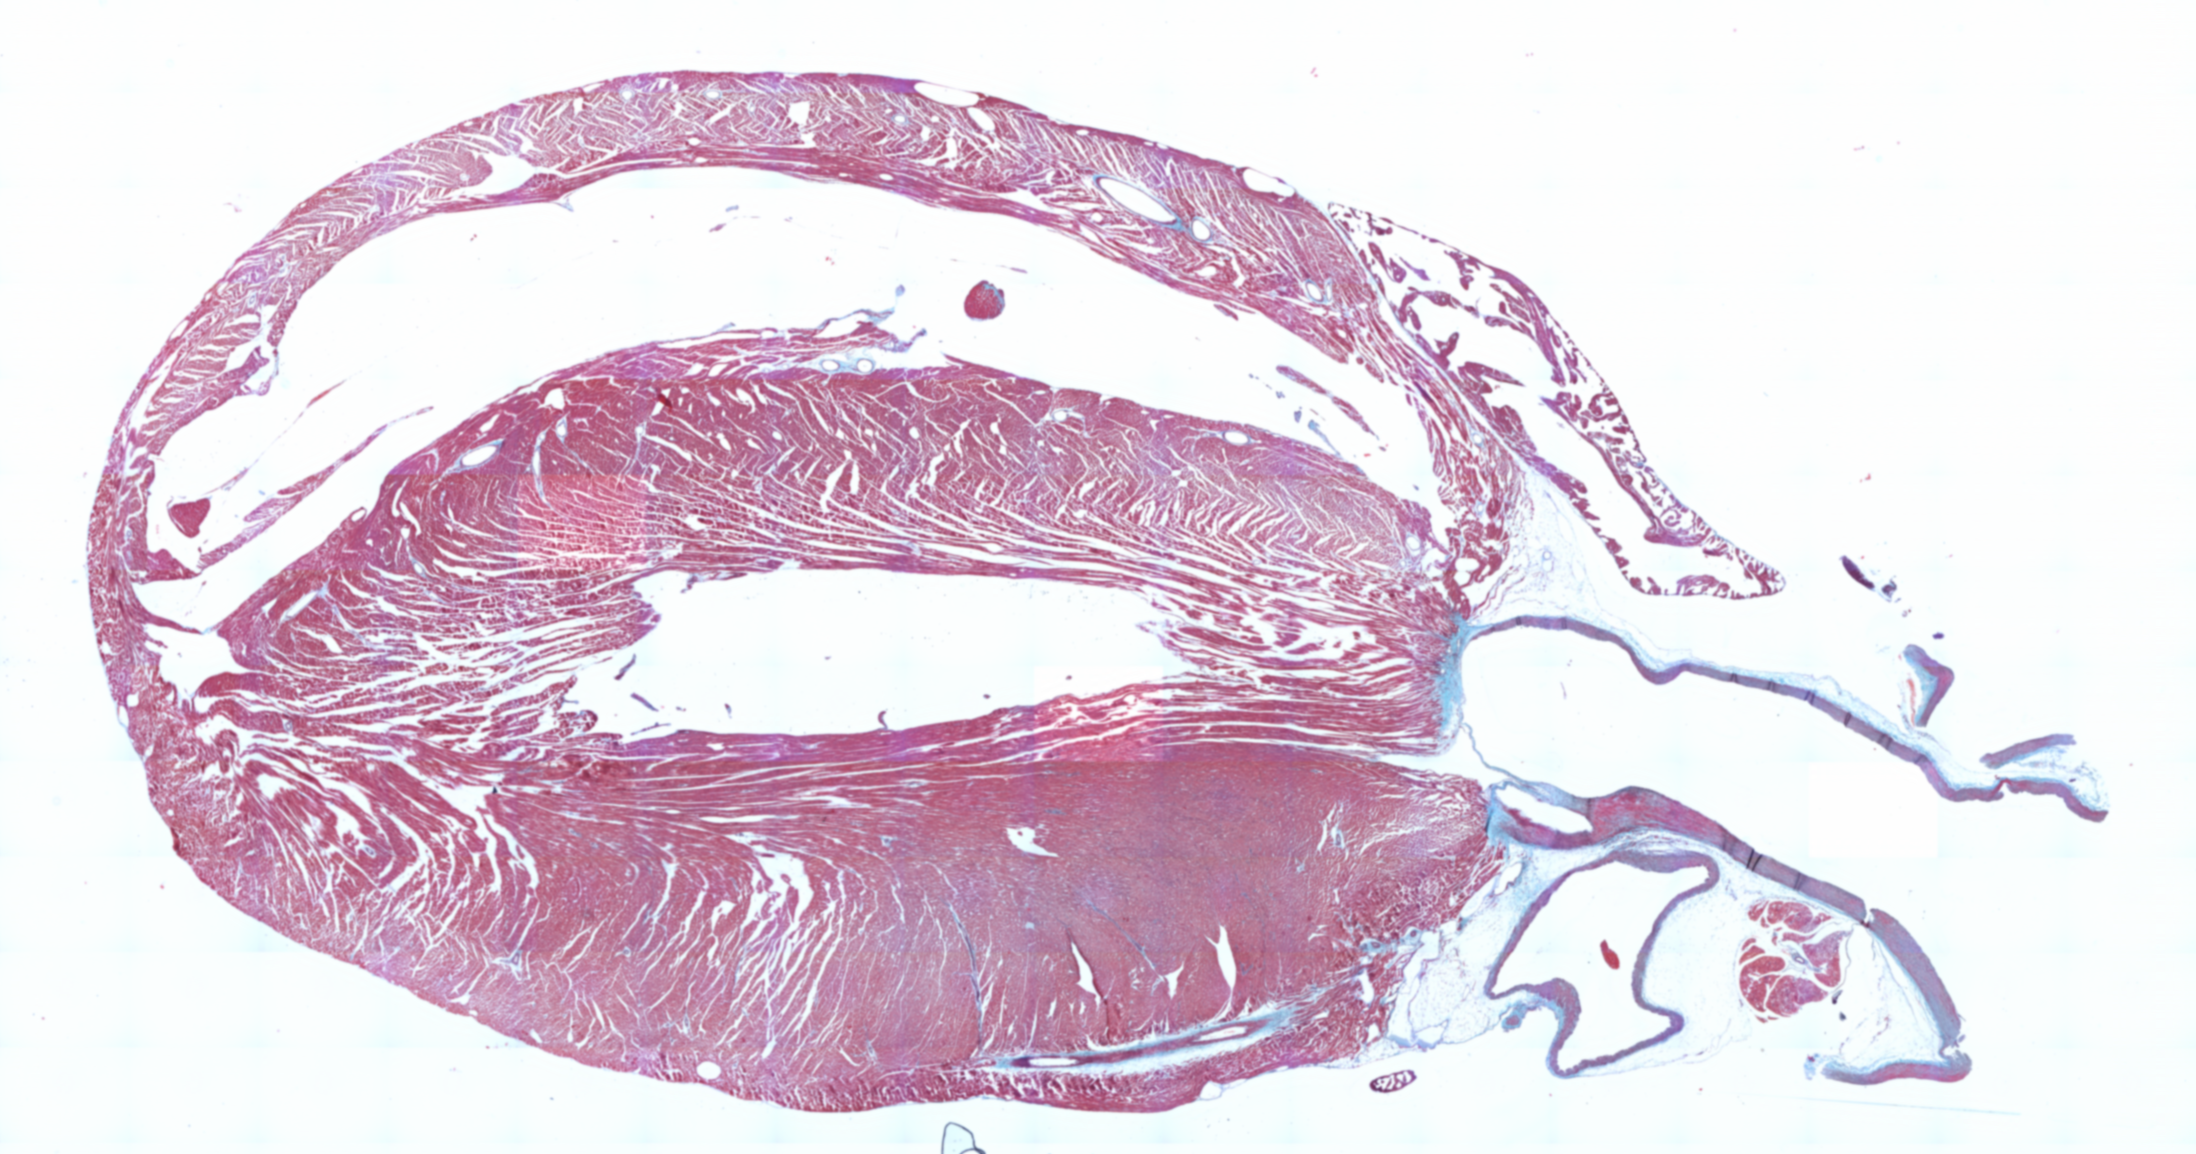
\includegraphics[width=0.8\pagewidth]{Ch5/Figs/HiRes_downsamples_8_0582}}
      \subfigure[][]{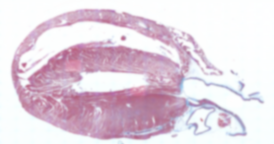
\includegraphics[width=0.8\pagewidth]{Ch5/Figs/HiRes_downsamples_64_0582}}
      \caption{Slice images of slice 582. \textbf{(a)} is Gaussian smoothed and downsampled by a factor of 8 to 8.8$\mu$m resolution, and \textbf{(b)} by 64 to 70.4$\mu$m resolution. The slice must be reflected and rotated in order to align with the block face image in Figure~\ref{fig:original_lores_images}.}
      \label{fig:original_hires_images}
    \end{figure}
	
  % subsection image_acquisition (end)

  \subsection{Image Curation} % (fold)
  \label{sub:image_curation}
    The images provided by Burton et al. \cite{Burton2006} discussed in Section~\ref{sub:image_acquisition} yield unprecedented detail and quality. Although every possible step was taken during image acquisition, certain unavoidable experimental practicalities arose. A master subset of the images was selected, removing any slices with unacceptable damage such as that found in Figure~\ref{fig:damaged_slice}. Wherever a slice or group of slices was missing or removed, the acceptable adjacent slices were repeated symmetrically to fill the gap, in order to preserve the macroscopic geometry of the tissue. In the rare case where two images of the same slice existed, both slices were examined and the higher quality version was selected.
    
    \begin{figure}[htbp]
      \centering
      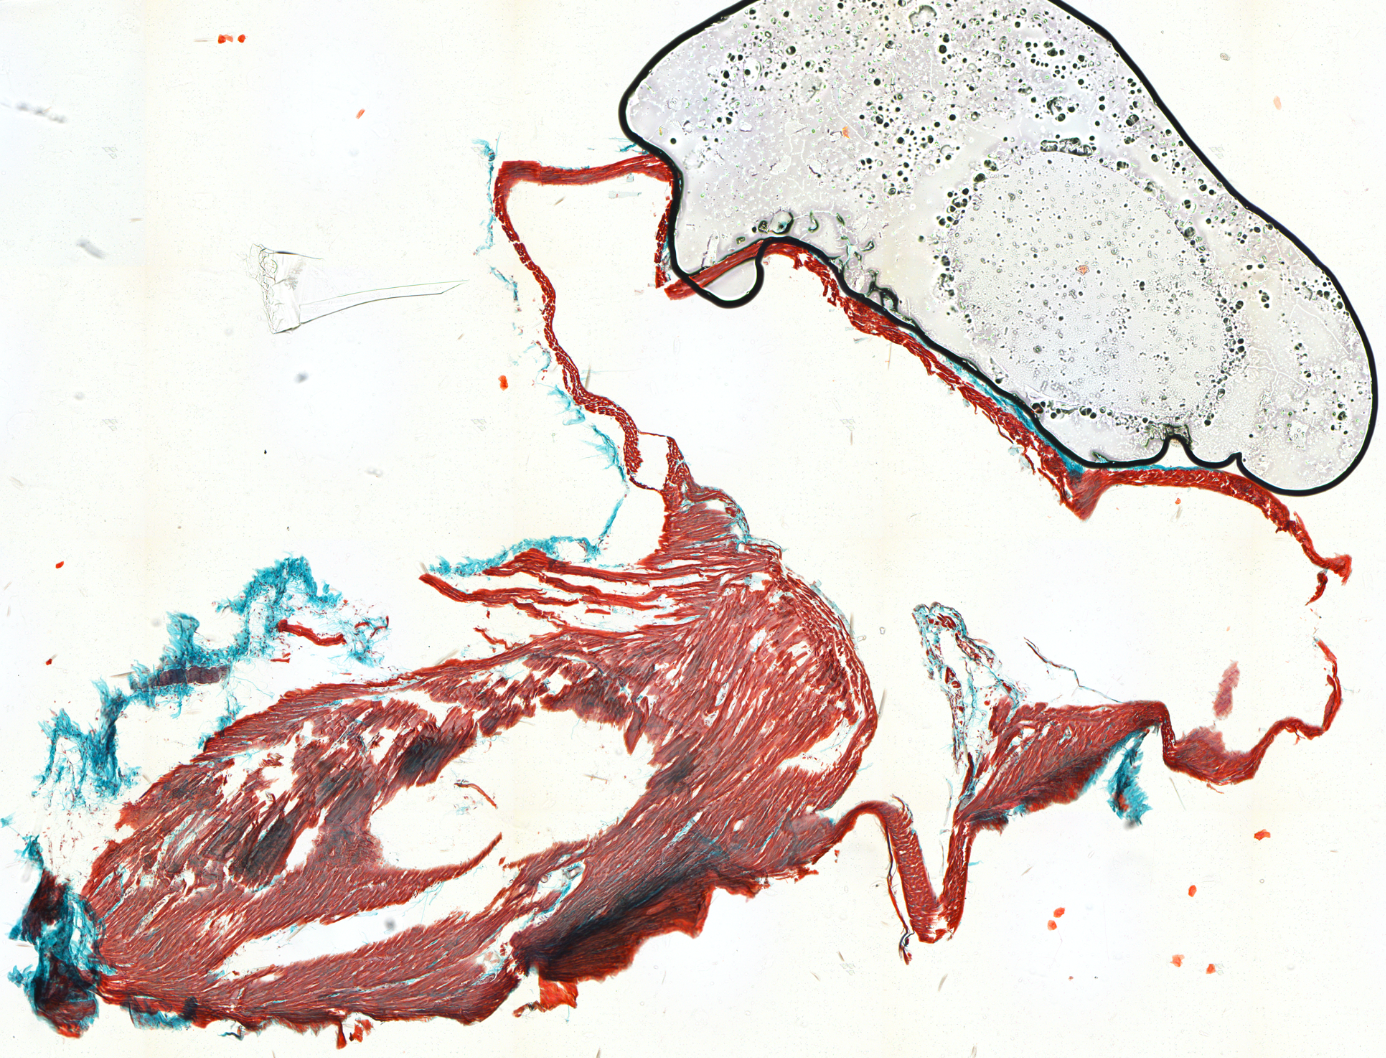
\includegraphics[width=.8\textwidth]{Ch5/Figs/damaged_slice}
      \caption{A damaged slice close to the left extremity of the heart. The tissue is severely damaged and folded in place. There is also a large bubble trapped between the two imaging slides.}
      \label{fig:damaged_slice}
    \end{figure}
    
  % subsection image_curation (end)
  
  \subsection{Image Preparation} % (fold)
  \label{sub:image_preparation}
  	The digital camera used to obtain the images created files with four channels: red, green, blue and alpha. Since transparency is meaningless in the context of a photograph, the fourth alpha channel was uniformly black. Unfortunately, the implementation of the RGBA BMP reader in ITK labels the channels incorrectly, so that the black alpha channel is interpreted as red, the red as green, the green as blue, and the blue as alpha. To correct for this, channels were explicitly permuted and the redundant alpha channel removed.
    
    On occasion, part way through image acquisition, the block face camera would be moved relative to the surface of the wax block. All images acquired from then on had to be translated and rotated to compensate for this movement. At each perturbation, the two slices between which the camera had moved were registered in order to calculate the corrective transform, which was then applied to all subsequent slices. In each case, the parameters shown in Table~\ref{tab:block_face_to_block_face} were used to optimise a centered rigid transform. Figure~\ref{fig:LoRes_cross_sections} depicts the results of these corrections, and the isosurface of the corrected segmented volume are shown from 6 sides in Figures~\labelcref{fig:LoRes_positive_x,fig:LoRes_negative_x,fig:LoRes_positive_y,fig:LoRes_negative_y,fig:LoRes_positive_z,fig:LoRes_negative_z}. The isosurface was generated from a threshold segmentation of the intensity magnitude of the volume, the threshold level being judged manually in order to overlap maximally with the true heart contour. A dense cloud of wax bubbles and other small artefacts obscured the main surface of the heart, and so a binary shape opening filter was applied to remove all but the largest connected region from the segmentation before the contour was extracted.
    
    % lores cross sections
    \begin{sidewaysfigure}[htbp]
      \centering
      \subfigure[][]{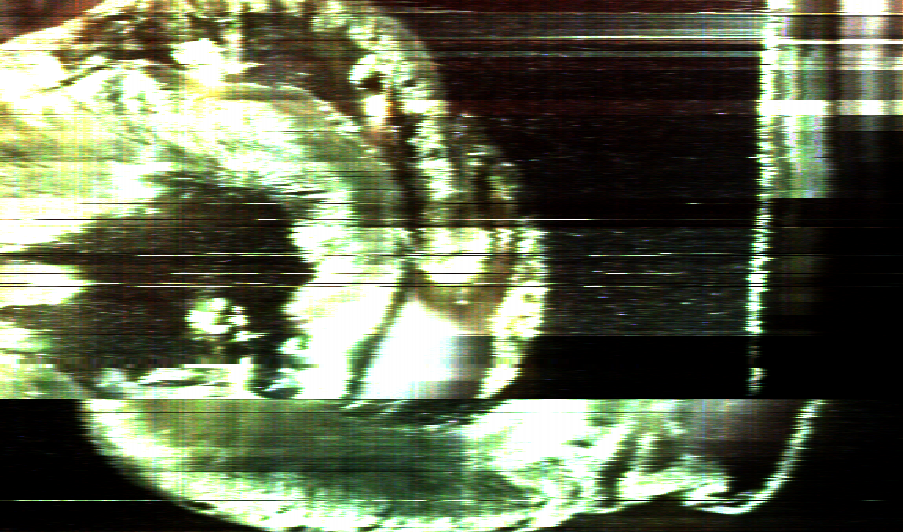
\includegraphics[height=0.31\textheight]{Ch5/Figs/LoRes_without_adjustments_0_235}}
      \subfigure[][]{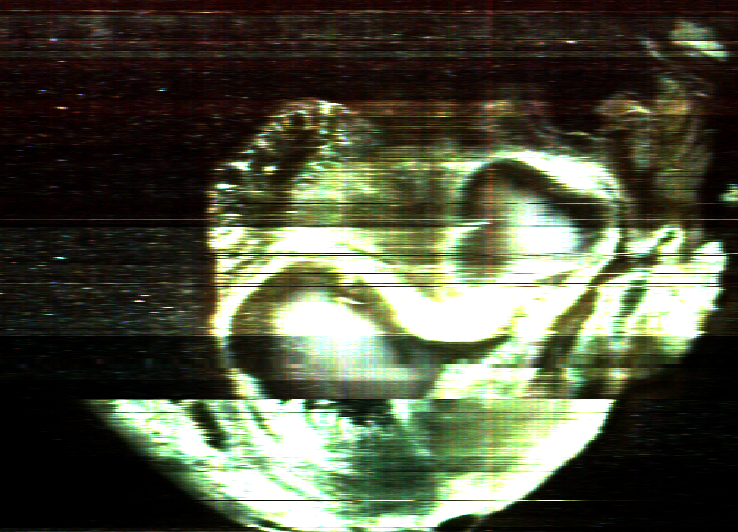
\includegraphics[height=0.31\textheight]{Ch5/Figs/LoRes_without_adjustments_1_287}}
      \subfigure[][]{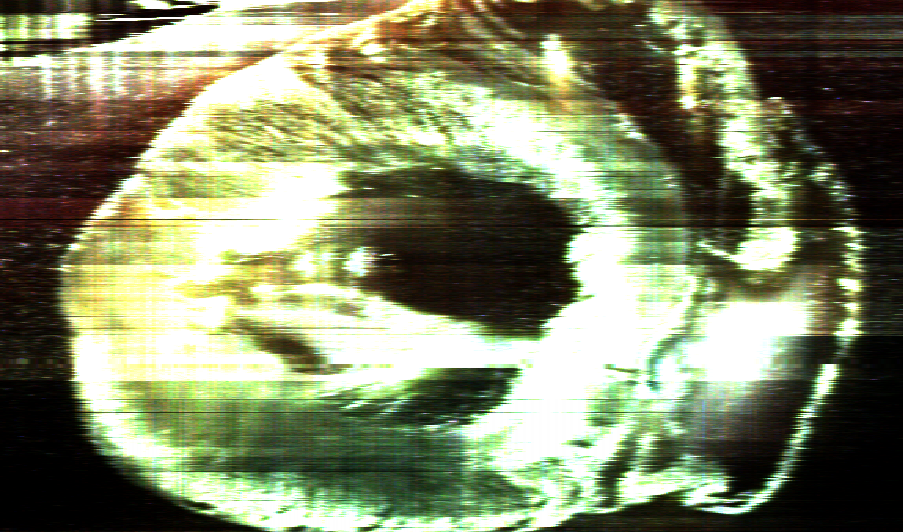
\includegraphics[height=0.31\textheight]{Ch5/Figs/LoRes_0_235}\label{subfig:LoRes_adjusted_long_cross_section}}
      \subfigure[][]{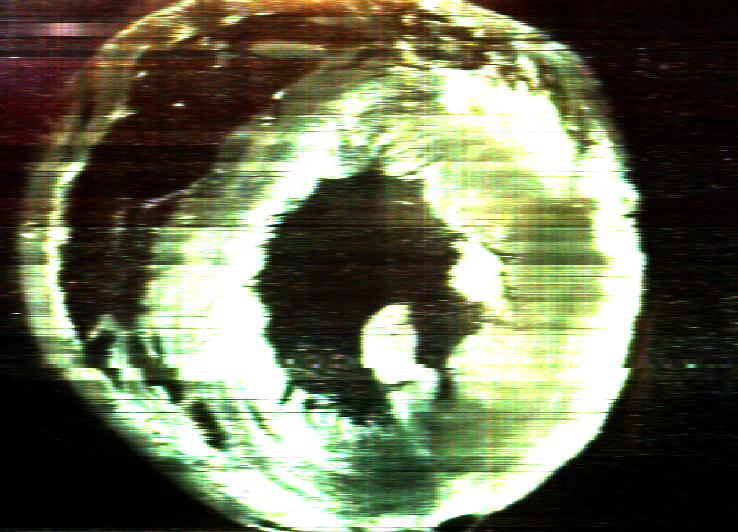
\includegraphics[height=0.31\textheight]{Ch5/Figs/LoRes_1_287}}
      \caption{Central cross-sections of the cropped block-face volume. \textbf{(a)} and \textbf{(b)} show the volume before adjustment, where a large camera displacement is apparent approximately a quarter of the way from the bottom of the image. Several thin stripes are visible further up, where the occasional single image has been displaced. The volume is fully aligned in \textbf{(c)} and \textbf{(d)}, with striations visible due to discrete changes in the positioning and intensity of illumination. These changes will propagate to the final registration result.}
      \label{fig:LoRes_cross_sections}
    \end{sidewaysfigure}
    
    % lores contours
    \begin{sidewaysfigure}[htbp]
      \centering
      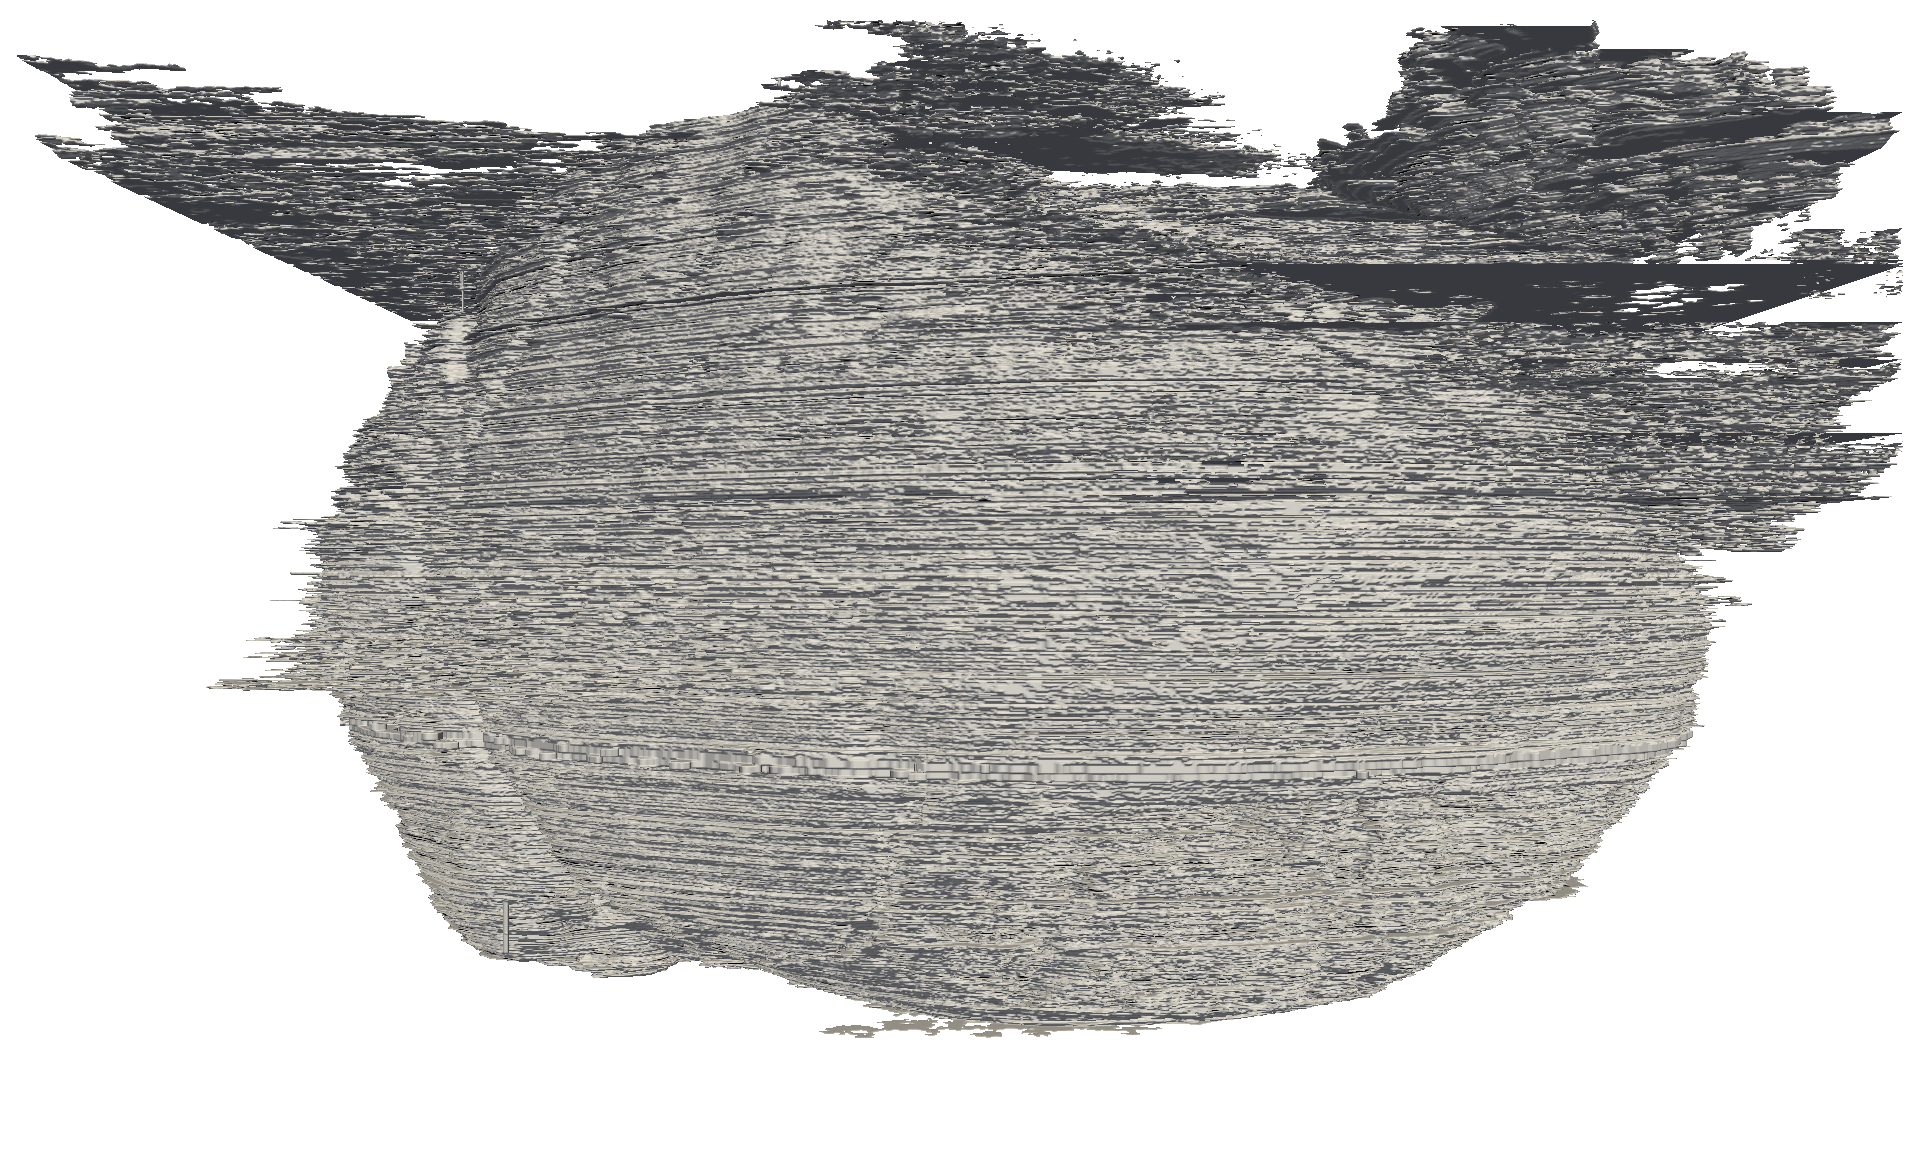
\includegraphics[width=\textheight]{Ch5/Figs/Rat28/contours/LoRes_positive_x}
      \caption{A contour of the adjusted block face volume, viewed along the positive x direction. The round surface of the heart apex is clearly visible to the right. Oddly shaped protrusions in the top third of slices are due to gradually brightening reflection from the suface of the wax.}
      \label{fig:LoRes_positive_x}
    \end{sidewaysfigure}
    
    \begin{sidewaysfigure}[htbp]
      \centering
      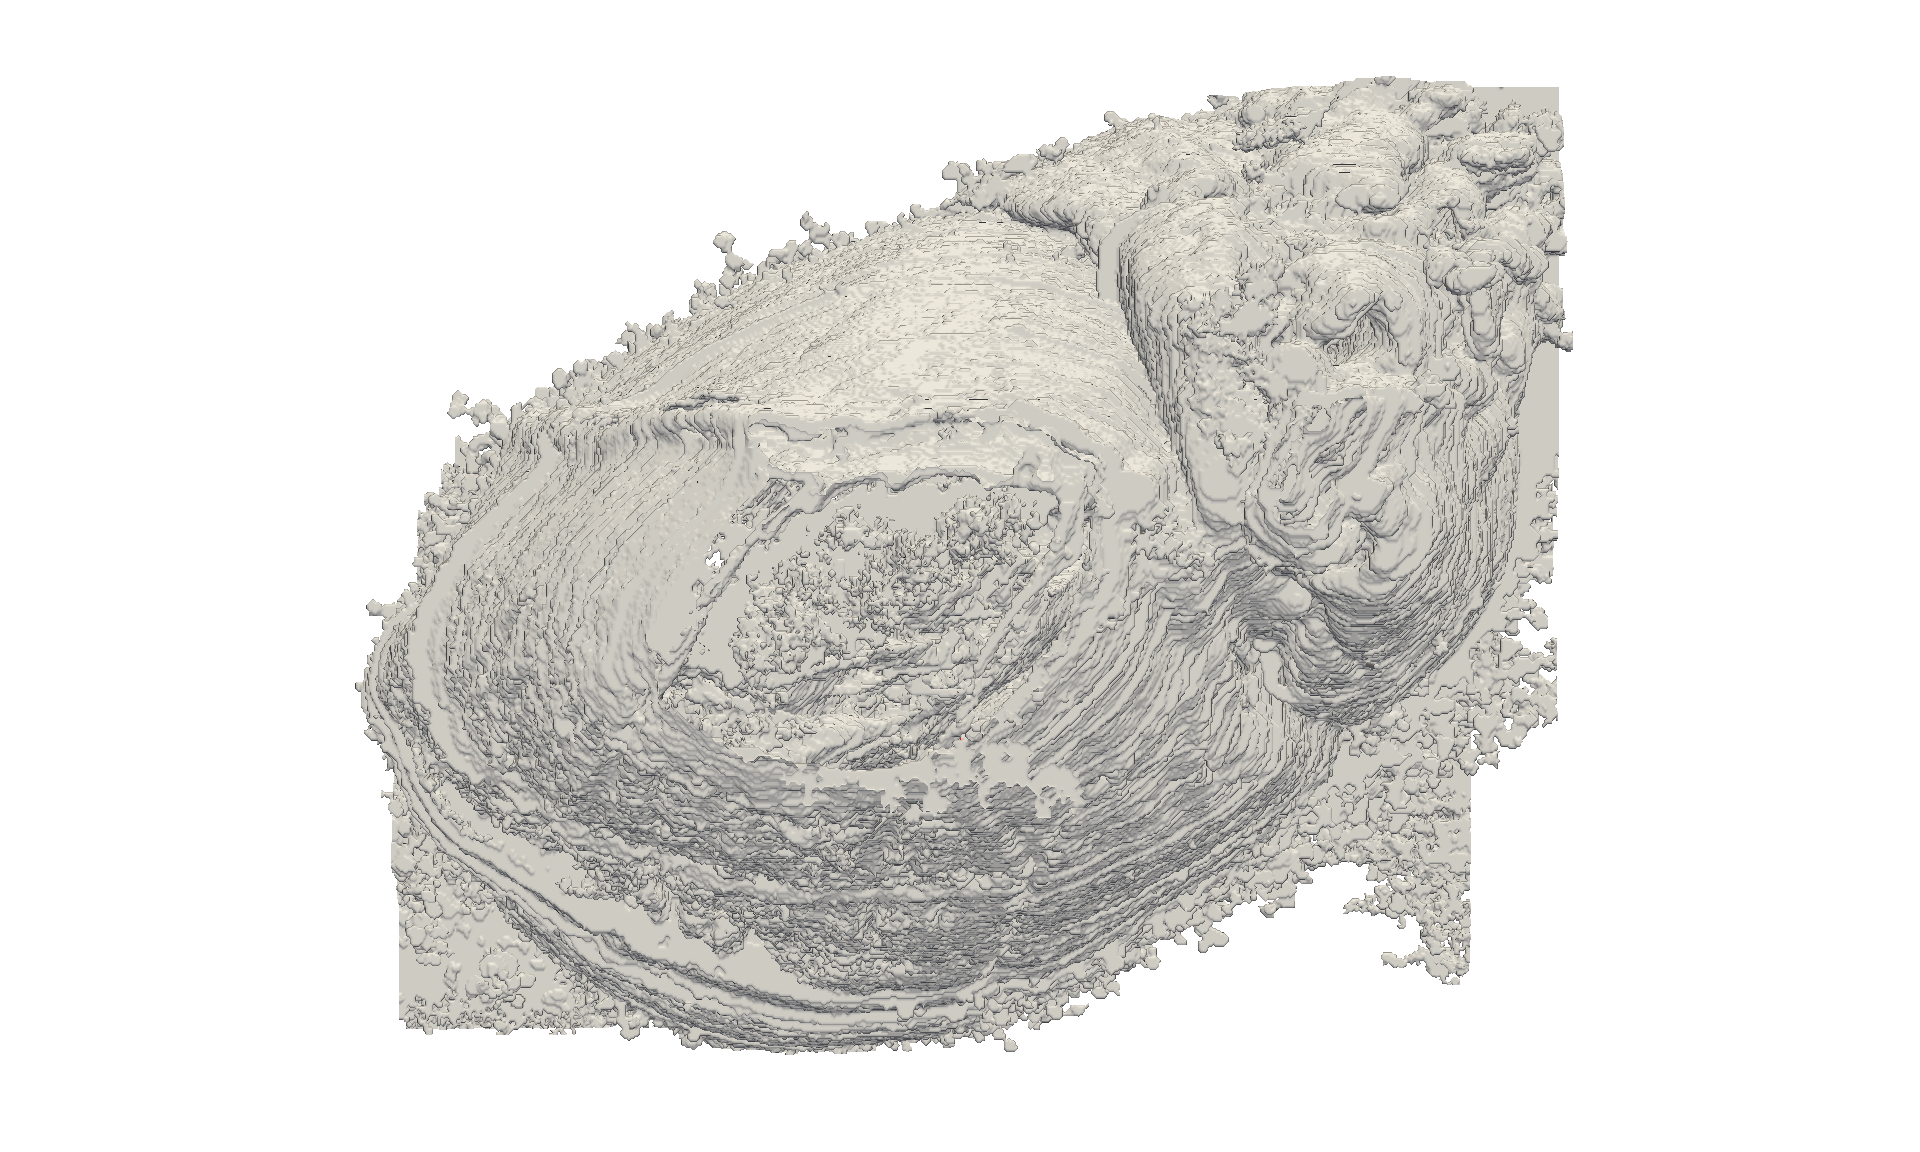
\includegraphics[width=\textheight]{Ch5/Figs/Rat28/contours/LoRes_positive_z}
      \caption{The block face contour viewed along the positive z direction. The detail and composition of the images is clearly visible from this angle. Note the protruding epicardial vessel in the top left. The surface of the first third of slices near the bottom left looks eroded, in a region where the threshold intensity values have failed to pick up the tissue boundary faithfully.}
      \label{fig:LoRes_positive_z}
    \end{sidewaysfigure}
    
	As is evident from Figures~\labelcref{fig:original_lores_images,fig:original_hires_images} for one slice, the vast majority of slices had been flipped over between sectioning from the block surface and being photographed. Slice images were therefore reflected across one axis in order to restore geometric parity with the associated block face image.
	
	 Several sets of downsamples of varying factors were generated, the lowest of which were used for debugging and testing, working up in detail, size and computational expense as the techniques were perfected. Before downsampling, a Gaussian smoothing was applied in each case, with sigma equal to the new larger pixel spacing. In this way, all original pixels in the region of a large downsampled pixel contribute to its final value, and aliasing noise problems associated with frequencies higher than half the downsampled pixel spacing are avoided. This results in a smoother and more accurate cost function. Figures~\labelcref{fig:original_lores_images,fig:original_hires_images} juxtapose the full images with various levels of downsampling.
	 
	 When registering two images, it is important that they are of comparable resolution, in order to minimise processing time and to ensure the smoothest possible cost function. In Figure~\ref{fig:downsample_zooms}, the effects of the downsampling can be seen more clearly. Individual cell nuclei are resolved at the highest resolution of slice image, but the maximum resolution block face images are of much lower detail. Clearly, the original slice images, with 1.1$\mu$m pixel spacings, are needlessly detailed compared to their block face counterparts, with a mere 26.6$\mu$m. As is discussed in Section~\ref{ssub:multiresolution_registration}, it is therefore appropriate to register slice images at a factor of 8 times more downsampled than the block face images.
    
	%  Lo/HiRes zooms
    \begin{sidewaysfigure}[htbp]
      \centering
      \subfigure[][]{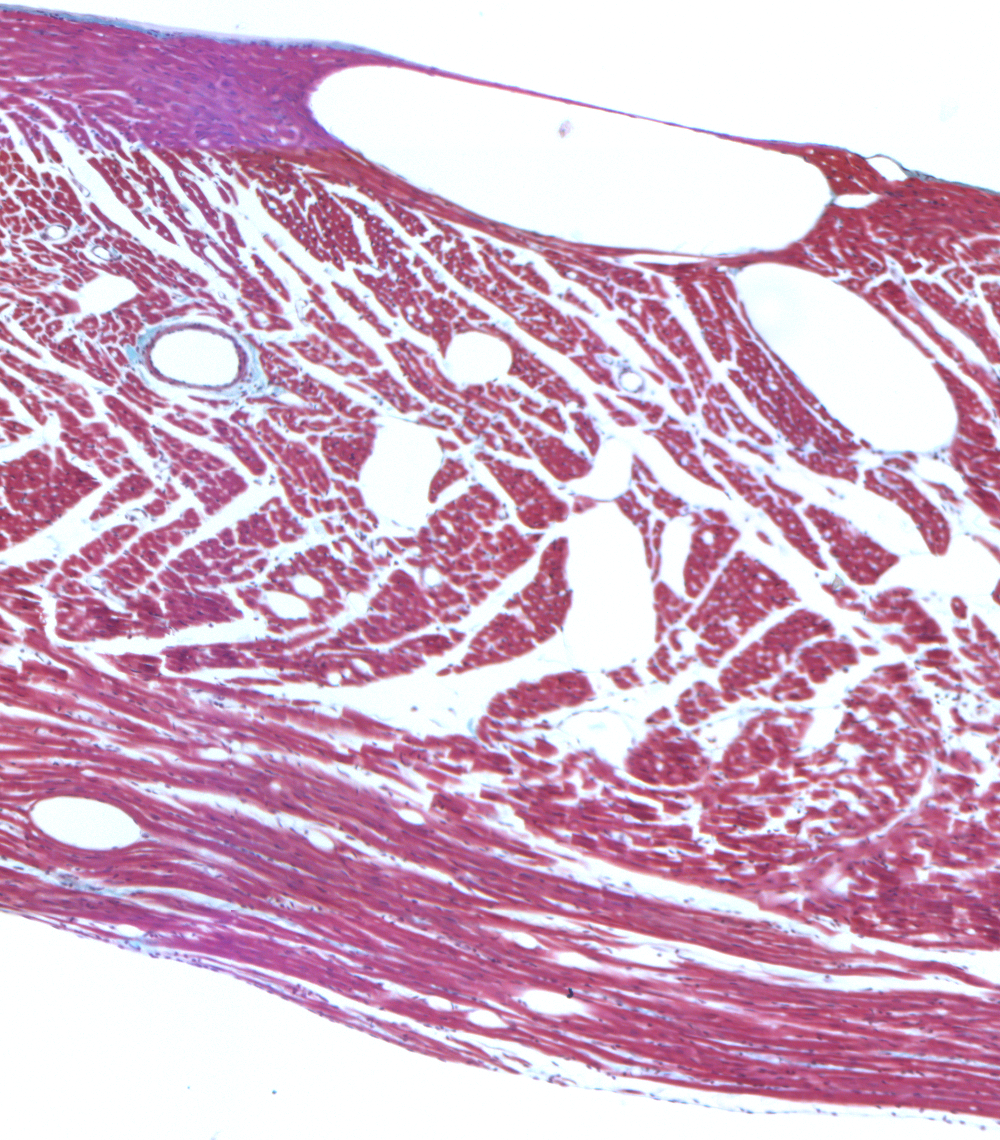
\includegraphics[width=0.39\pagewidth]{Ch5/Figs/HiRes_downsamples_1_0582_zoom}}
      \subfigure[][]{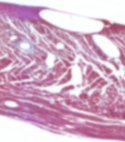
\includegraphics[width=0.39\pagewidth]{Ch5/Figs/HiRes_downsamples_8_0582_zoom}}
      \subfigure[][]{
\includegraphics[width=0.39\pagewidth]{Ch5/Figs/HiRes_downsamples_64_0582_zoom}}
      \subfigure[][]{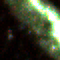
\includegraphics[width=0.39\pagewidth]{Ch5/Figs/LoRes_rgb_downsamples_1_0582_zoom}}
      \subfigure[][]{
\includegraphics[width=0.39\pagewidth]{Ch5/Figs/LoRes_rgb_downsamples_8_0582_zoom}}
      \caption{An epicardial vessel in slice 582 of Rat 28, in both the slice and the block face images. \textbf{(a)}, \textbf{(b)} and \textbf{(c)} show the slice original, 8x and 64x downsampled, while \textbf{(d)} and \textbf{(e)} show the block face original and 8x downsampled. The fibres parallel to the internal wall at the bottom of \textbf{(a)} are angled such that they reflect the illumination strongly at the top right of \textbf{(d)}, and are in much sharper contrast to the black wax than the rest of the tissue. Indeed, they are in much sharper contrast to the rest of the tissue than the rest of the tissue is to the non-tissue.}
      \label{fig:downsample_zooms}
    \end{sidewaysfigure}
  % subsection image_preparation_and_curation (end)
  
  \subsection{Initialisation} % (fold)
  \label{sub:initialisation}
    In general, the optimisation algorithms used in registration do not assure convergence to the global minimum and are thus sensitive to initialisation and to the presence of local minima in the cost function. A reasonable initialisation is necessary for robust and accurate registration.
	
		\subsubsection{Geometric Initialisation} % (fold)
		\label{ssub:geometric_initialisation}
			The block face images are already coherent from their acquisition. White space under the microscope surrounding the slices had already been cropped, such that each slice sat approximately centrally within the bounds of its image. Having been reflected across the x-axis, an anticlockwise rotation of $90\,^{\circ}$ oriented most slices approximately with the block face, as is seen from Figures~\labelcref{fig:original_lores_images,fig:original_hires_images}. A small set of slices required $180\,^{\circ}$ rotations. Slice images were then initialised to their common centre to form a volume. The initial translation and pixel spacing of the block face volume was then manually tuned to overlap maximally with the slice volume. As is exhibited in Section~\ref{sec:results}, this na\"ive geometric initialisation provides an adequate starting point.
		% subsubsection geometric_initialisation (end)
	
		\subsubsection{PCA Initialisation} % (fold)
		\label{ssub:pca_initialisation}
			Although geometric initialisation provided a reasonable starting point for most slices, this was purely a consequence of how the experimentalist had manually obtained and cropped the original images. A more sophisticated method might make use of the information in the image. If the pixels containing tissue could be identified, the centres of mass and principal components of each pair of images can be aligned to provide a close initial matching.
		
		  Various segmentation methods were tested in an effort to identify tissue reliably in both sets of images. Because the block face volume was already coherent, volume-wise refinements and filters could be applied, whilst only 2D segmentation techniques could be considered for the slice images.
			
			After applying any image preprocessing, such as a gradient magnitude or Hessian filter, many segmentation methods, such as opening and closing or level sets, are designed to improve, and in particular connect, the edges or surfaces of an approximate segmentation. Yet here in the context of rigid transforms, it is to be noted that only the segmentation's moments are of consequence, in particular the centre of mass and the variance matrix. It is therefore unnecessary for the segmentation to overlap closely with the tissue at a small scale, only that the global distribution of tissue be represented precisely. That being said, methods to remove macroscopic artefacts, such as connected component filtering and selection proved beneficial in most contexts.
			
		  There is no facility to align the principal components of two images in ITK, only to align their centres of mass. The class itk::CenteredTransformPCAInitializer was implemented to encapsulate the details of this process. The results of applying this class compared to the simple geometric initialisation are shown in Figure~\ref{fig:582_pca}, and the segmentations upon which they are based are shown in Figure~\ref{fig:582_segmentation}.
		
	    It is somewhat clear from Figure~\ref{fig:LoRes_cross_sections} that the broad range of tissue colours and intensities in the block face volume overlap significantly with the colours and intensities of non-tissue. In Figures~\labelcref{fig:582_segmentation,fig:582_pca}, the threshold segmentation values were optimised for these particular slices as a proof of concept, but this slice was chosen as one of the best examples of the technique. Issues such as wax bubbles, the bright blob at the top of the block face volume, optical transmission from layers below, and differential brightness from differing fibre directions or anatomical features plagued efforts to segment the images, and in fact went on to plague registration. Even if a segmentation method could yield reasonable results for every slice in the dataset, it is impractical to tune parameters manually for each slice, and there would certainly not be a single parameter set suitable for every slice in the volume. For these reasons, the PCA method could not be used to improve robustly upon a simple geometric initialisation of the high-resolution slices seen in Figure~\ref{fig:geometric_initialisation}.
    
	  \begin{figure}[htbp]
	    \centering
      \subfigure[][]{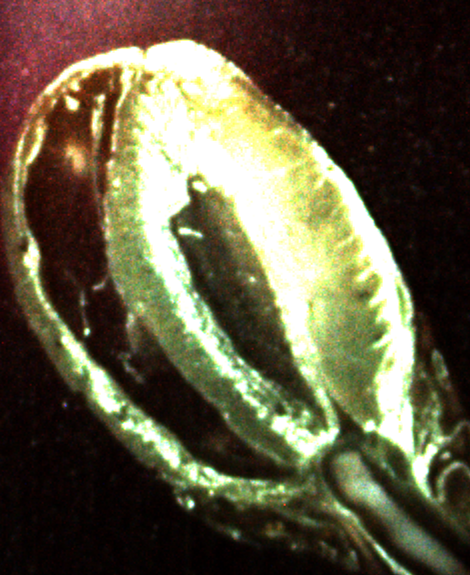
\includegraphics[width=0.4\pagewidth]{Ch5/Figs/pca/LoRes_562}}
      \subfigure[][]{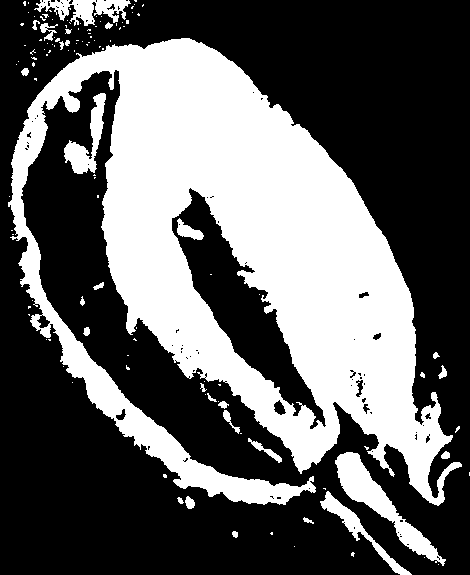
\includegraphics[width=0.4\pagewidth]{Ch5/Figs/pca/LoRes_segmentation_562}}
      \subfigure[][]{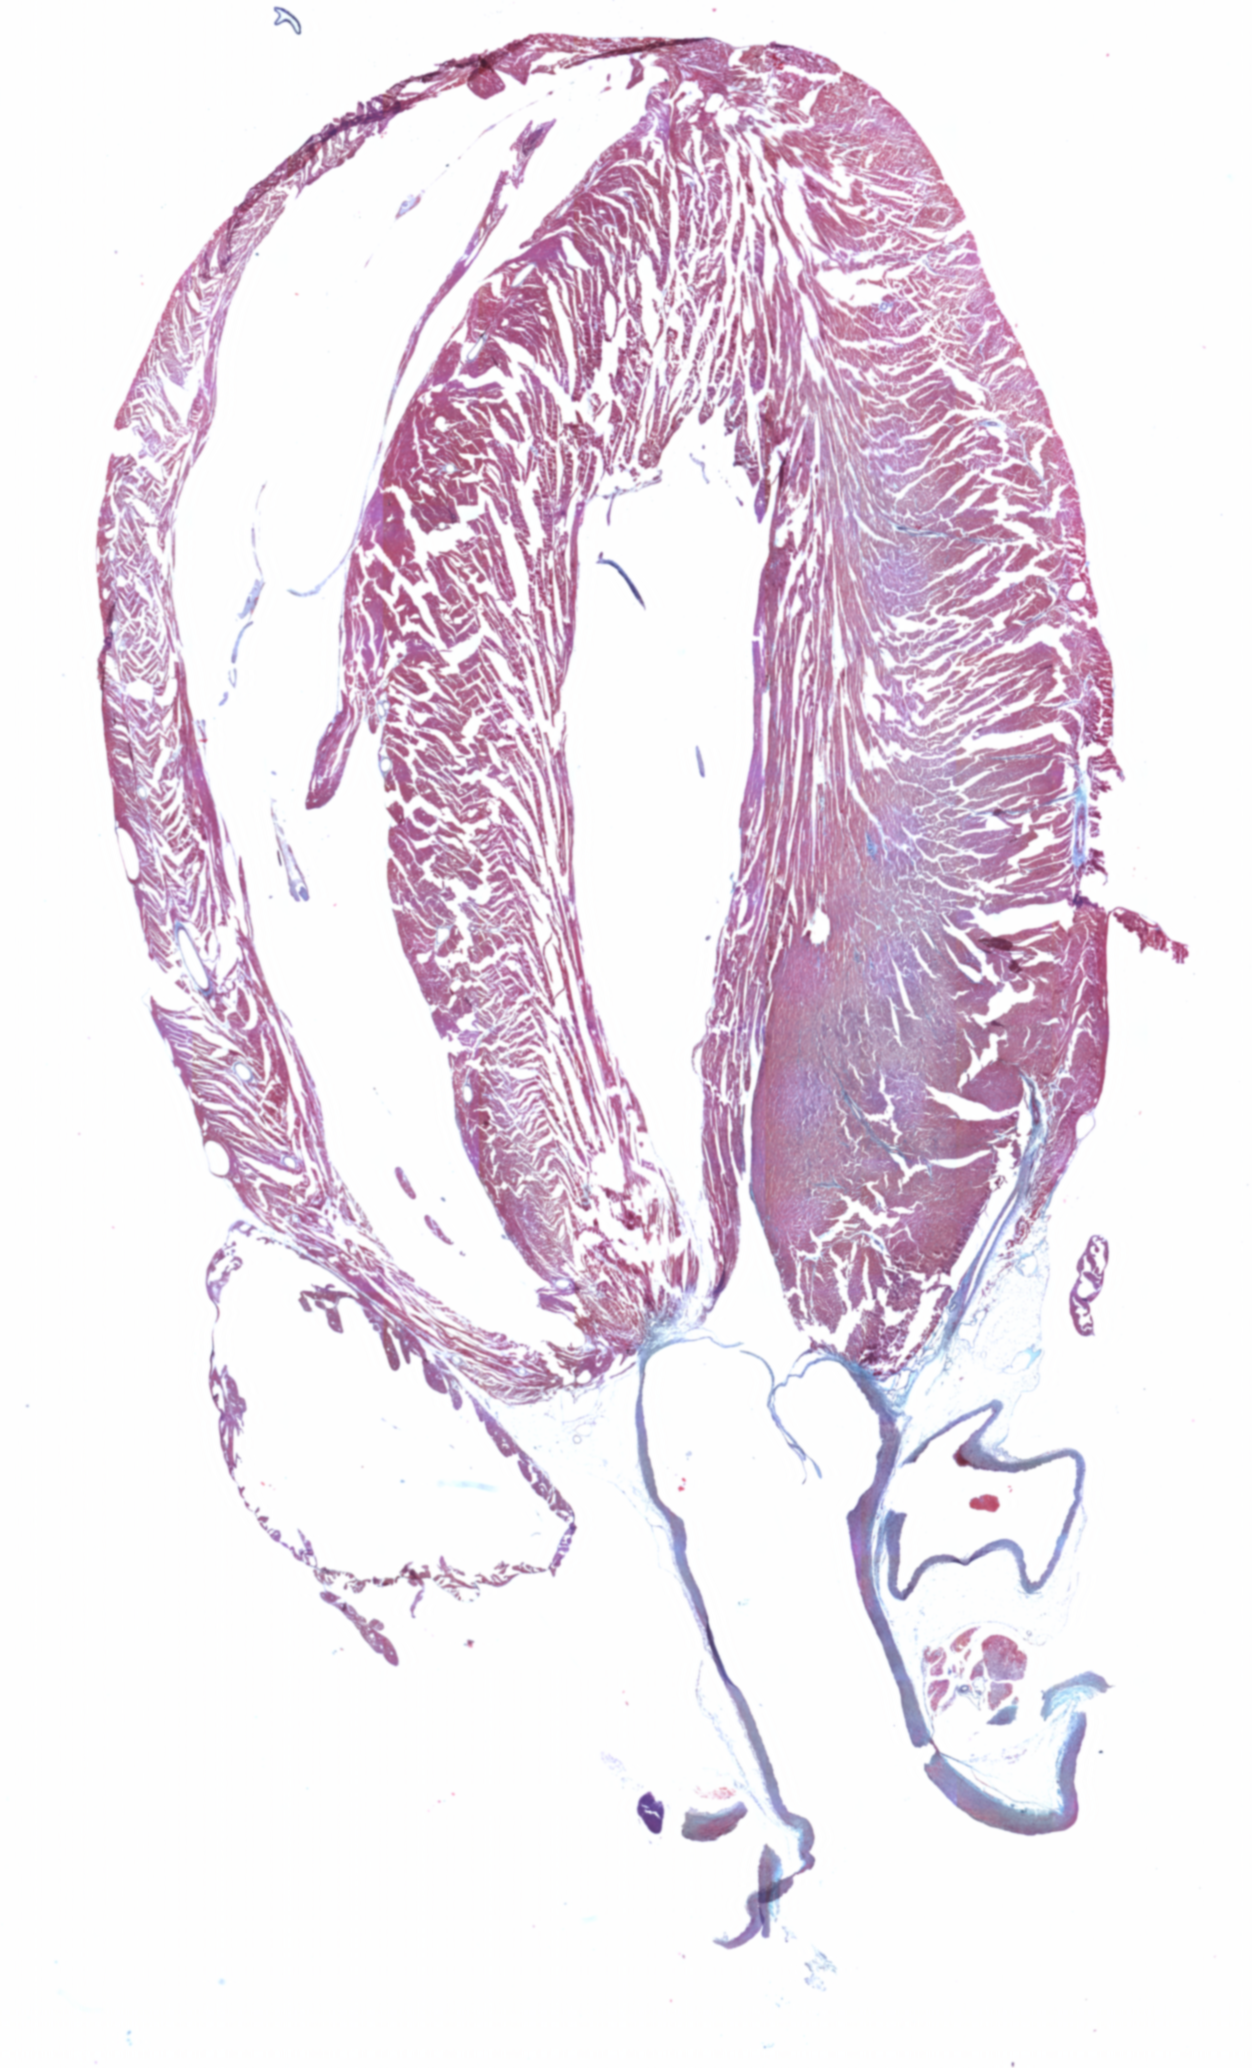
\includegraphics[width=0.4\pagewidth]{Ch5/Figs/pca/HiRes_562}}
      \subfigure[][]{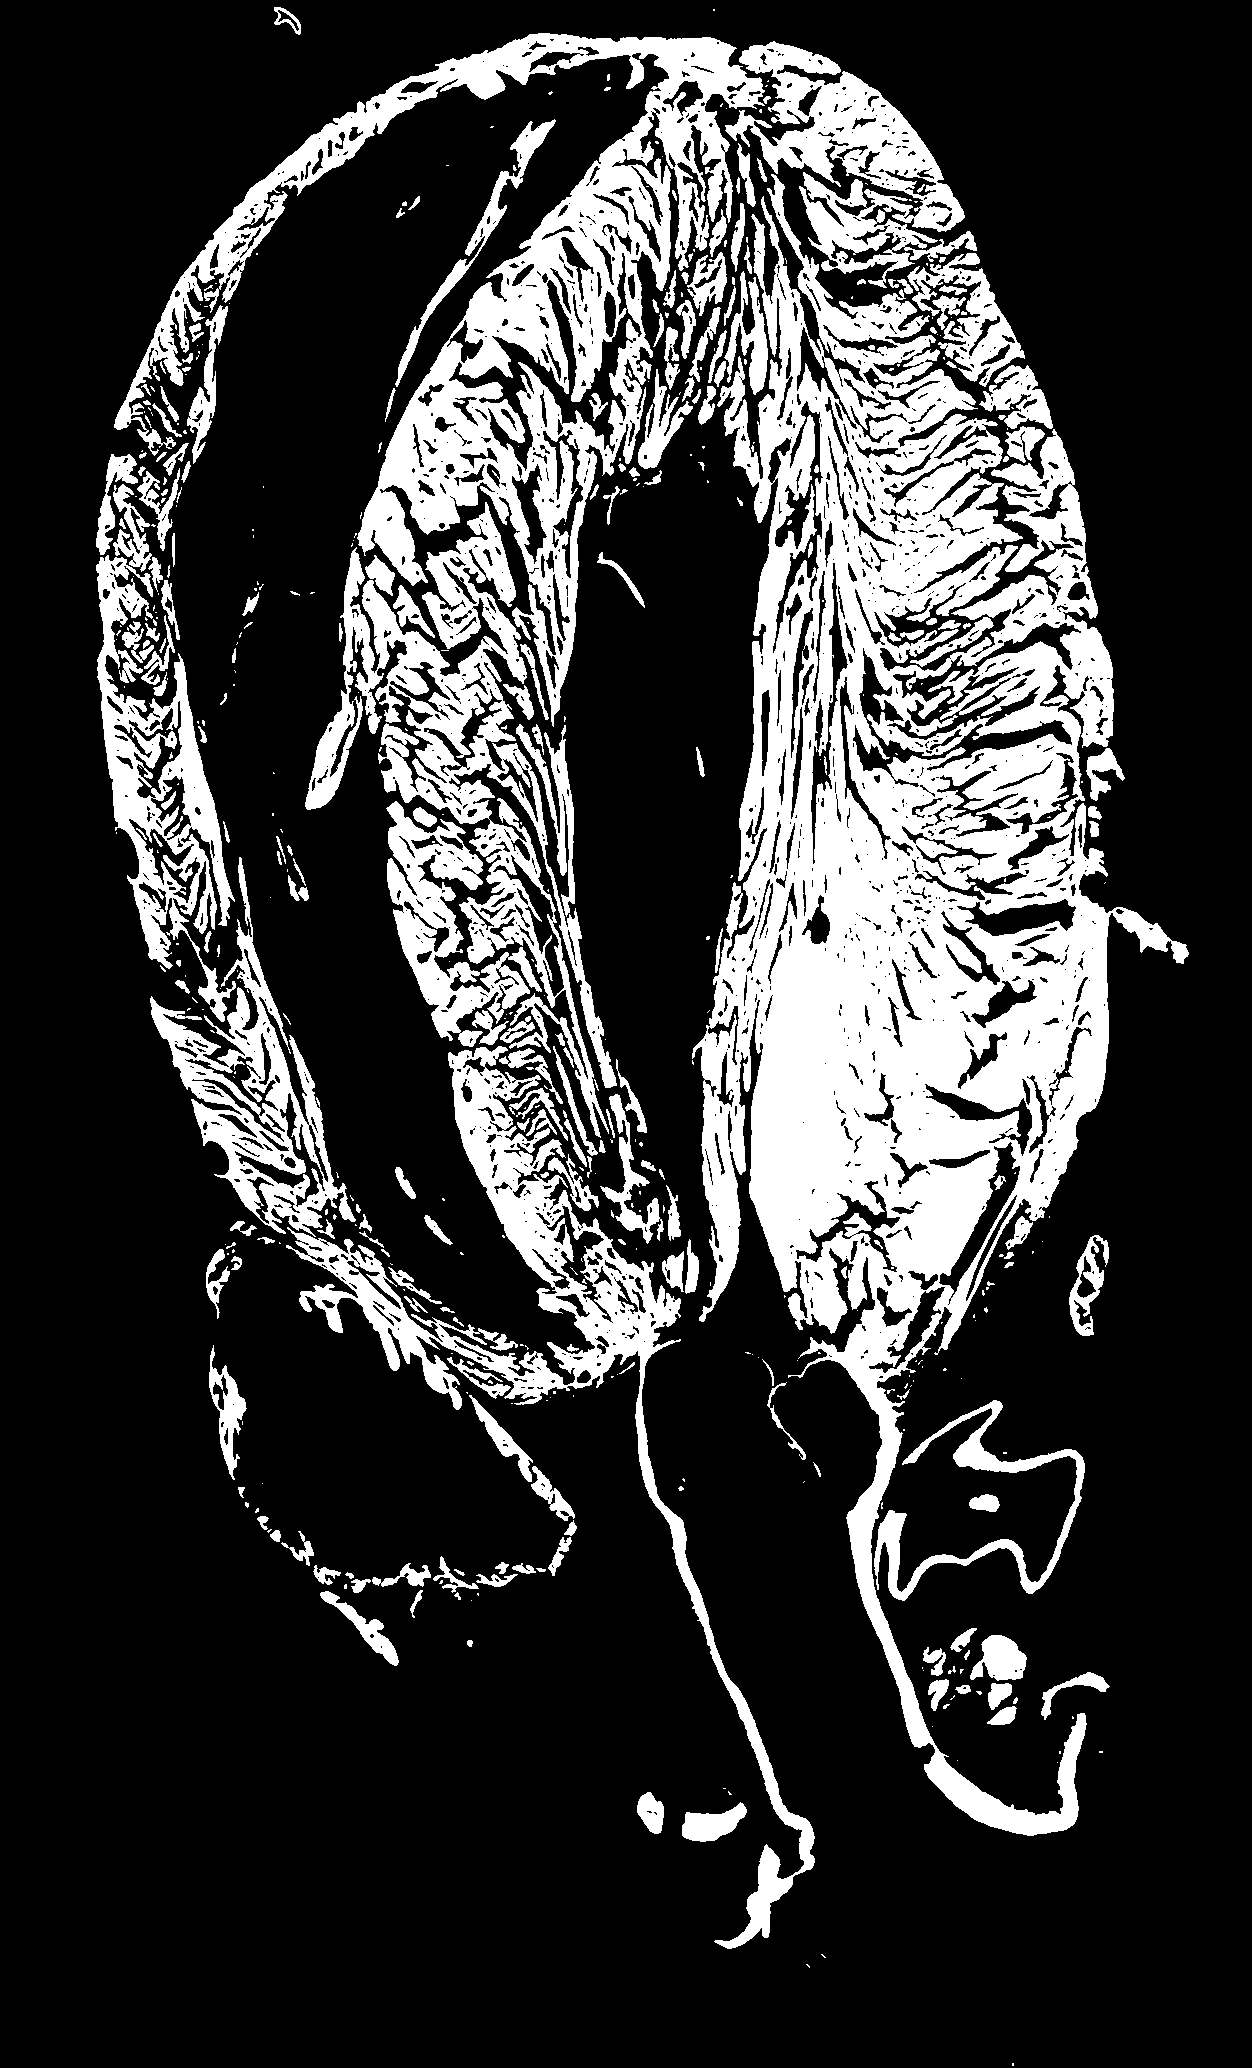
\includegraphics[width=0.4\pagewidth]{Ch5/Figs/pca/HiRes_segmentation_562}}
      \caption{Originals and threshold segmentations of the block face and slice images of slice 582.}
	    \label{fig:582_segmentation}
	  \end{figure}
    
	  \begin{figure}[htbp]
	    \centering
      \subfigure[][]{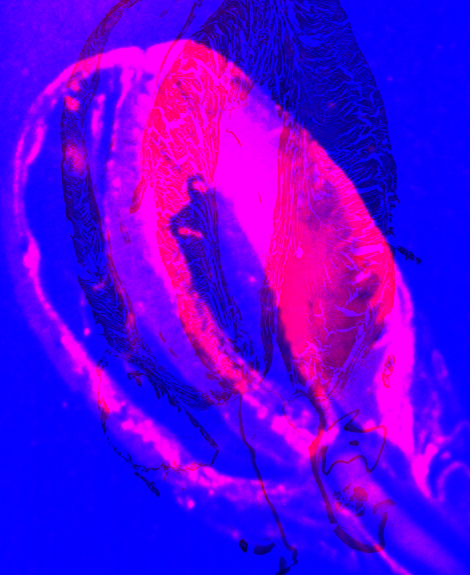
\includegraphics[width=0.4\pagewidth]{Ch5/Figs/pca/geometric_redblue}}
      \subfigure[][]{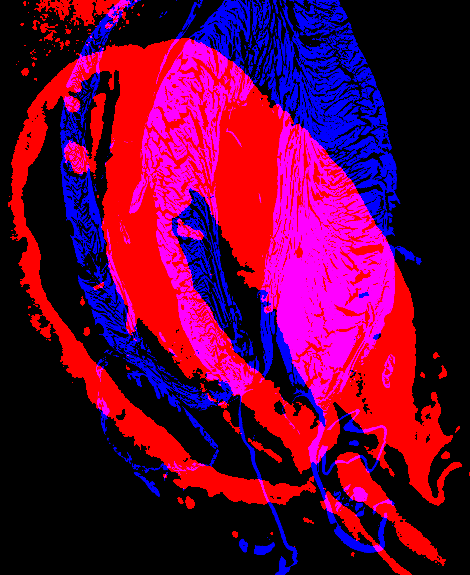
\includegraphics[width=0.4\pagewidth]{Ch5/Figs/pca/geometric_segmentation_redblue}}
      \subfigure[][]{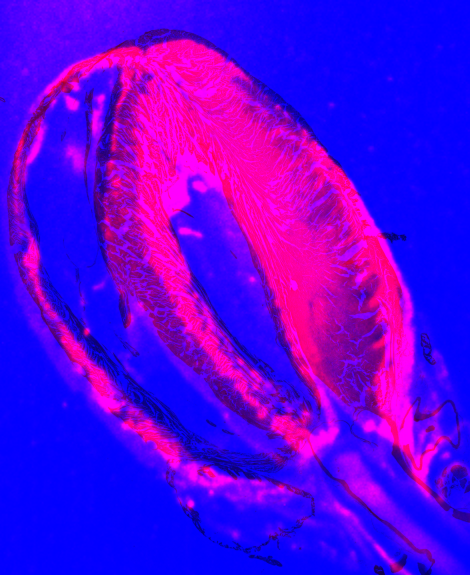
\includegraphics[width=0.4\pagewidth]{Ch5/Figs/pca/pca_redblue}}
      \subfigure[][]{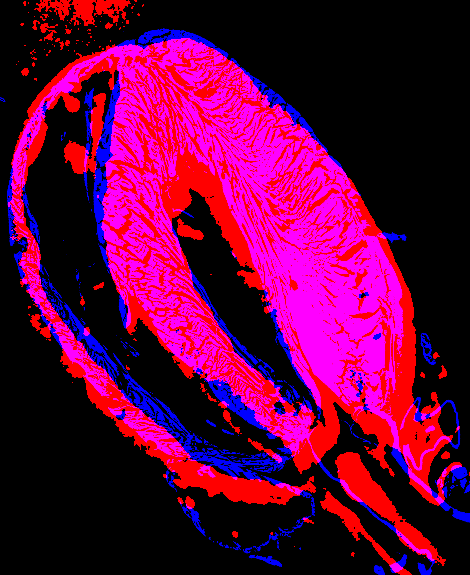
\includegraphics[width=0.4\pagewidth]{Ch5/Figs/pca/pca_segmentation_redblue}}
      \caption{Intensity superpositions of block face (red channel) and slice (blue channel). The original images are used \textbf{(a)} and \textbf{(c)}, while the segmentations are shown in \textbf{(b)} and \textbf{(d)}. \textbf{(a)} and \textbf{(b)} show geometric initialisation, and \textbf{(c)} and \textbf{(d)} PCA initialisation. It is clear that PCA provides a much closer match from which the registration algorithm can begin.}
      \label{fig:582_pca}
    \end{figure}
    
		% subsubsection pca_initialisation (end)
  % subsection initialisation (end)
  
	\subsection{Registration Algorithm} % (fold)
  \label{sub:registration_algorithm}
    Each main aspect of the registration method is outlined in this section. A well-founded registration algorithm must embody three traits: numerically, it must converge reliably to the global minimum; computationally, it must be efficient so as to be tractable; and physically, it must correspond to the process that it was designed to correct for. It is through the lens of these three benchmarks that we examine the following components.
    
    \subsubsection{Transforms} % (fold)
    \label{ssub:transforms}
			The sectioning of the slices introduces 2D, slice-specific deformation and in some cases damage. The subsequent relaxing and rehydration of each slice causes further deformation. A large proportion of this deformation will be of similarity or affine form. By first registering the simplest of transforms with the lowest dimensional parameter space, and then incrementally relaxing transformational constraint by increasing the number of parameters, we can provide the best possible starting point in each higher dimensional parameter space.
			
      Transforms were optimised in the following order, the final result of each initialising its successor: a centered rigid 2D transform - a rotation about an arbitrary centre followed by a translation; a centered similarity transform - as before but with a scaling factor; and a centered affine transform - an affine transformation around an arbitrary centre followed by a translation. For all transforms, the centre of rotation was exposed for optimisation as metric parameters. Finally, a coarse grid and subsequent fine grid bspline deformable transform was tested, but found to be unstable. Further research outside of this thesis would likely lead to better results.
    % subsubsection transforms (end)
    
    \subsubsection{Metrics} % (fold)
    \label{ssub:metrics}
      Mutual Information (MI) is usually considered to be most effective when registering images from different modalities \cite{Wells1996}. However, after a plethora of parameterisations and configurations was explored based on this metric with little success, incrementally simpler and simpler metrics were tested. Each demanded more image preconditioning and tuning, but yielded monotonically closer and more consistent registrations, with a larger capture range, and required fewer iterations to converge. First, a normalised correlation was employed, with the simplest mean squares difference algorithm proving most suitable. It would appear that the simpler the intensity relationship, the smoother the cost landscape, with fewer local minima. Scalings were initially chosen based on the dimensions of the images, and subsequently tuned using the diagnostic techniques discussed in Section~\ref{sub:diagnostics}.
    % subsubsection metrics (end)
  
    \subsubsection{Optimisation} % (fold)
    \label{ssub:optimisation}
      Gradient Descent (GD) and Regular Step Gradient Descent (RSGD) optimisers from ITK have been applied. In the ITK implementation of RSGD, registration terminates before the maximum number of iterations has passed, based on either a minimum step length or a minimum gradient magnitude tolerance. Thus in simple cases, RSGD is computationally more efficient. In most scenarios, however, the GD optimiser often proves more robust, since anomalous cost function topologies can sometimes shorten the RSGD step length multiplier prematurely. In both cases, a choice to maximise or minimise the cost function must be chosen, the latter being dependent on both the choice of metric and the preconditioning of the image intensity ranges.

      The optimisation space, as dictated by the transform, must be scaled along each dimension to correct for discrepant effects per unit change of each parameter. For example, a translation of one micron at the epicardium might result from a rotation of just $10^{-5}$ radians about the centre of the slice. This makes the metric space more isotropic and reduces the eccentricity of cost function basins, allowing the optimisation algorithm to fall more directly toward minima.
    % subsubsection optimisation (end)
	% subsection registration_algorithm (end)
    
  \subsection{Software Architecture} % (fold)
  \label{sub:software_architecture}
		From early on, the requirements of the problem diversified, and a range of related tools were built. Because the final result was unknown, it was often extremely difficult to know whether the code was operating correctly. Bugs or errors in calculation were not usually apparent, and proved very difficult to find. For these reasons, significant effort was aimed at building code that was robust, reusable, efficient and parallelisable, that facilitated repeated trials, allowing processing of large datasets and that provided tools for analysis of intermediate results and evolution during the algorithm. Common patterns and functionality needed to be extracted and isolated. This prevented duplication and the potential for bugs and inconsistencies, and lead to more readable and manageable code. We outline the main problems encountered during the development process, along with the solutions crafted to isolate and overcome them.
		
		\subsubsection{Languages and Frameworks} % (fold)
		\label{ssub:languages_and_frameworks}
      All file handling and networking algorithms were written in the Ruby programming language. Imaging algorithms were written in C++ or, in some simple cases, Python, using ITK. C++ executables were compiled using the cross-platform build system CMake. YAML was used as a declarative language for configuration files, providing a syntax that is easily human readable and curatable, yet machine parsable. Source code management and code deployment was implemented in Git, and the project is freely available at \url{http://github.com/mattgibb/registration} under an MIT license.
		% subsubsection languages_and_frameworks (end)
		
    \subsubsection{Stacks} % (fold)
    \label{ssub:stacks}
      Each block image must be paired with its equivalent slice image, and blank images must be interpolated where images are missing. Slices must be transformed independently and by a range of transform types. Resampler spacings must be set according to the original image spacings and the downsample ratios. Binary masks must be generated for each image, so that metrics will only take pixel intensities into account from inside the boundaries of the original untransformed images. A stack volume must be reconstructed from the transformed, resampled slices. A minimum percentage overlap is required for many metrics to function, and for small slice images close to the apex of the heart, block mask areas must be cropped until this constraint is satisfied.
	  	
      A hierarchy of Stack classes has been developed - along with associated builder classes, IO helpers and transform converters - to encapsulate the solutions to all of these problems. A Stack represents the 3D composition of a set of 2D slices. It handles ROI selection, generic transform storage, image and mask resampling and generation (both for 2D slices and for the 3D volume) and various error handling strategies. An MRI class is also available to solve the complementary problem of extracting arbitrarily oriented slices from a 3D image. However, for these specific datasets the block face images are intrinsically registered to the histological samples.
    % subsubsection stacks (end)
    
    \subsubsection{Multiresolution Registration} % (fold)
    \label{ssub:multiresolution_registration}
			The total size of the block face and slice images approaches two terabytes \cite{Gibb2012} and pose significant challenges for computational processing and visualisation \cite{Goodyer2009}. Even with an 8x downsampled slice dataset, one full rigid registration to test one parameter set would take nearly 100 hours on a modern quad core processor. An affine registration performed with a regular step gradient descent optimizer is parameterised in 10 dimensions. Rapid feedback is required if the right parameters are to be found in any reasonable time, and so a multiresolution approach must be taken. There are 2 ways to reduce the resolution of the dataset: in-plane downsampling and out-of-plane slice selection.
			
      In-plane downsampling and Gaussian smoothing not only reduces time, but smooths the cost function and can lead to more robust registration results. In multiresolution registration, the resulting transforms can then be used to initialise a more accurate but more fragile registration at a higher resolution.
			
      To start with, a quick order-of-magnitude overview of the global performance of a particular parameter set was required. In this case, regularly spaced subsets of the full curated list were created, such as every thirtieth slice or every fifth slice. Alternatively, every slice within a region might be selected, for example, the band of slices spanning an epicardial vessel. Of course, these two reductions can be applied together for very rapid feedback. As will be made clearer in Chapter~\ref{cha:diffusion_smoothing_registration_of_high_resolution_rat_histology}, full out-of-plane resolution is required to parameterise effectively the coregistration of adjacent slices. However, the fruitful region of parameters near the apex of the heart for elliptical discs of tissue is different (yet not disjunct) from that in more complex, central slices. In this case, a group of representative slice sublists at full resolution, e.g. 100-110, 200-210, 300-310 etc., provide the best compromise between speed and accuracy.
			
			The slice list is loaded dynamically by all tools from a central config file, and so switching between lists when prototyping is as simple as redirecting a symlink.
    % subsubsection multiresolution_registration (end)
    
    \subsubsection{Builders} % (fold)
    \label{ssub:builders}
      A minimal registration pipeline is composed of several generic actors, including a metric, an optimiser, a transform, and an interpolator. The details of which types of actors are optimal and how they should interact are peculiar to the registration problem at hand. Furthermore, the specific type of each component often requires unique configuration beyond the generic interface of its family, and the choice of image preprocessing is dependent on the choice of metric. Once several types must be chosen from and configured, even for just one component, an ad hoc procedural approach quickly became unwieldy. These two requirements colluded combinatorially to demand a great deal of testing, tailoring and configuration in order to achieve registrations of high quality. More often than not, modifications would degrade the registration.
			
      The `Gang of Four' proposed the first categorised set of recurring solutions to common problems in object-oriented software design \cite{Gamma1995}. Three patterns they introduce are the Builder Pattern, the Abstract Factory Pattern and the Strategy Pattern. The Builder Pattern and the Abstract Factory Pattern are closely linked, both in their purpose and in their implementation; the Builder Pattern focusses on the construction of a single, complex object, whilst the Abstract Factory Pattern constructs a family of related or dependent objects. The Strategy Pattern encapsulates a group of concrete algorithms behind a generic interface, and makes them interchangeable with respect to any application code that employs them.
      
      At the pipeline level, we developed a hierarchy of frameworks employing the Builder pattern \cite{Gamma1995}, whose purpose is to abstract away the heavy lifting of wiring up the various components together. At the component level, a conflation of the Abstract Factory and the Strategy patterns \cite{Gamma1995}, together with a configuration system using the human-friendly YAML markup language, serves not only to decouple the actors' representations from the minutiae of their construction, but to move these volatile decisions from compile-time to runtime. These tools vastly reduce the cost of experimentation and testing. With all the variables clearly grouped together, with no need to recompile the toolchain or pore through source code to find if and where one can make a change, the feedback from results is faster and less error prone.
      
			The StackAligner class encapsulates the registration process, for tools employing affine or b-spline deformable transforms, across the whole heart or in a region of interest. At least two sets of stack configurations were required, for the block face and slice stacks, across a great many registration and reconstruction tools. This logic was pulled into a StackBuilder class tree, rooted from an untemplated StackBuilderBase class to prevent template infection across the codebase.
    % subsubsection builders (end)
		
		\subsubsection{Events, Checkpointing and IO} % (fold)
		\label{ssub:events_checkpointing_and_io}
			It is necessary to save intermediate information about the progress of the registration, for parameter tuning and analysis. ITK exposes this functionality through the Command Observer pattern \cite{Gamma1995}. Any ITK object can publish events, and other objects may subscribe to those events. An object whose purpose is to subscribe to an event and perform an action when that event is triggered is called a Command Observer. Figure~\ref{fig:command_hierarchy} shows the class tree developed to display and record the required information.
			
    \begin{figure}[htbp]
      \centering
      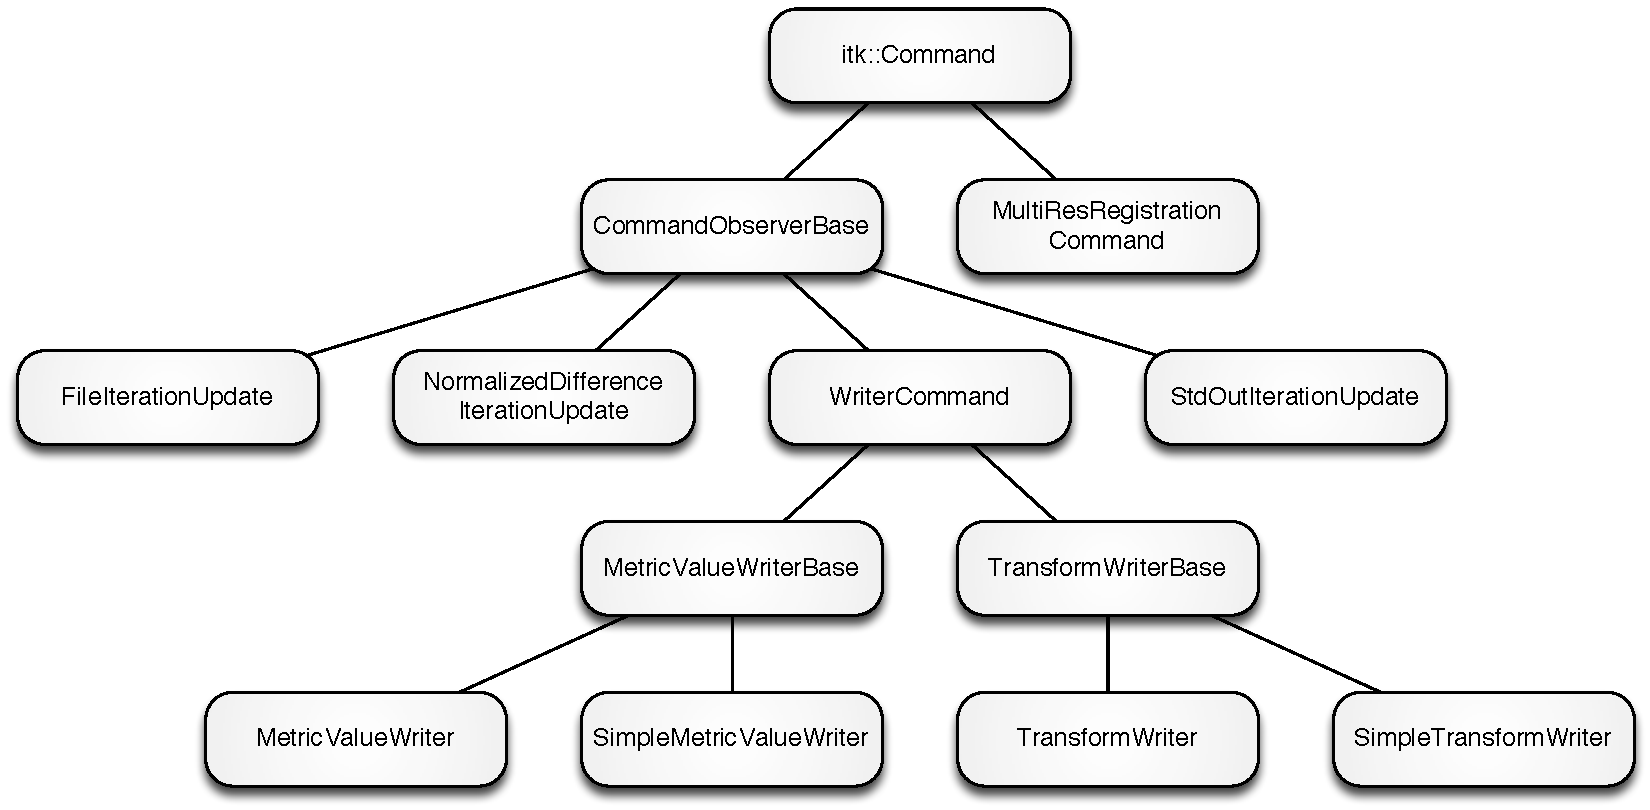
\includegraphics[width=\pagewidth]{Ch5/Figs/command_hierarchy}
      \caption{Command Observer hierarchy to output various types of information when specific events are triggered.}
      \label{fig:command_hierarchy}
    \end{figure}
		
      At any stage during the registration process, the vector of transforms held by a given Stack can be persisted to a series of files with a single function call. Just as easily, a new Stack can be initialised with a set of transforms on storage. This machinery facilitates greater process granularity in three dimensions: in the sequence of transforms to be optimised, in the increasing image resolutions to be registered, and spatially in the pairs of slices within the Stack. In the first case, a user can tune one registration stage until they are happy that it is optimal, and then use the results as a starting point for all subsequent runs of the next stage. In the second case, approximate registrations can be performed with images at lower resolutions, which can then initialise registrations at higher resolutions with different images. In the third case, the result from separate jobs for each slice pair using images of a scalar floating point pixel type or a segmentation image type can be aggregated and used to reconstruct a colour volume, perhaps at a different resolution. This division of workload and memory is of particular importance when organising jobs on clusters and shared memory machines.
			
			Even aside from process granularity, working with transforms is vastly superior to working directly with the images. Composing transforms rather than repeatedly resampling prevents a loss of image quality due to rasterisation in differing coordinate systems. Advanced composition of transforms makes possible registration refinement, either in regions of interest, or with the diffusion smoothing techniques discussed in Chapter~\ref{cha:diffusion_smoothing_registration_of_high_resolution_rat_histology}.
          
      Several other aspects of the architecture are not discussed here, including configuration, file management, testing, as well as the opportunities and challenges posed by high performance computing. These solutions are comprised mostly of generic software engineering practices and considerations, and are not relevant to the specific registration problem at hand.
		% subsubsection events_checkpointing_and_io (end)
		
  % subsection software_architecture (end)
  
  \subsection{Diagnostics and Parameter Tuning} % (fold)
    \label{sub:diagnostics}
      For almost a year and a half, it was very difficult to see why registration was failing to yield robustly accurate results. The output of raw transform values was somewhat elucidating, but only for obvious issues such as parameter scaling and step length, where almost zero change in some or all parameters signalled what to adjust. The space of possible parameters was enormous, and the computing time before feedback significant. With visual representation of nothing but the final result, determining which parameters to change and how was perhaps analogous to deciding how each player in a sports team could improve given only the final scores.
      
      Armed with the intermediate transforms and metric values discussed in Section~\ref{ssub:events_checkpointing_and_io}, the causes of the suboptimal registration results were immediately apparent. The progression of metric values for all slices could be plotted in graphs like those in Figures~\labelcref{fig:rigid_metric_values,fig:similarity_metric_values,fig:affine_metric_values,fig:affine_metric_value_differences}. Progress volumes of a particular slice could be constructed as seen in Figures~\labelcref{fig:progress_cross_sections,fig:progress_contour}.
			
			The regular step gradient descent optimiser is parameterised with four values: two behavioural values (maximum step length and relaxation factor), and two cutoff values (minimum step length and gradient magnitude tolerance). Bad behavioural values manifest in static or `zigzagging' unstable progress volumes and metric values, whilst premature or overcautious cutoff values yield either no region or a needlessly large region of equilibrium at the end. Bad parameter scaling is not evident solely from the intermediate metric values, which can still remain smoothly increasing with a quasi-equilibrated final section. However, the progress volume will appear restricted in one or more dimension. For example, the slice may rotate freely, but remain at a fixed translation, despite an obvious translational cost gradient.
			
			Not all symptoms could be diagnosed. In rare cases, the metric value would gradually and consistently worsen, and it was unclear why this was happening. Perhaps an oddly shaped cost basin or saddle point was to blame, deepening steeply along one dimension and shallowly along a perpendicular one.
    % subsection diagnostics (end)
% section methods (end)
   
\section{Results} % (fold)
\label{sec:registration_results}
	The work leading up to this chapter is composed of a great many dead ends and failed experiments, but consequently, we can assert with confidence that the results presented here are the best that can be achieved with these methods. Details of computation times are followed by the plotting of intermediate and final metric values. The progress of a single representative slice is scrutinised, ending with cross-sections and contours of the registered histological volumes after each successive registration.
	
  To begin with, lower resolution images were used to approximate parameters in reasonable time, but all registrations shown here were eventually performed with the full resolution block face images and 8x downsampled slice images. On a MacBook Pro with a 2.4GHz Intel Quad Core i7 processor, registering the original block face image to an 8x downsampled slice image took approximately 0.25 seconds per iteration. For the 1500 iterations required for rigid registration, and for 900 slices, this extrapolates to 93 hours total run time. When jobs were distributed on the cluster, 12 parallel registrations could be run concurrently in times of low demand. The total registration time was reduced from 93 hours to just below 7 hours.
	
  \begin{sidewaysfigure}[htbp]
    \centering
    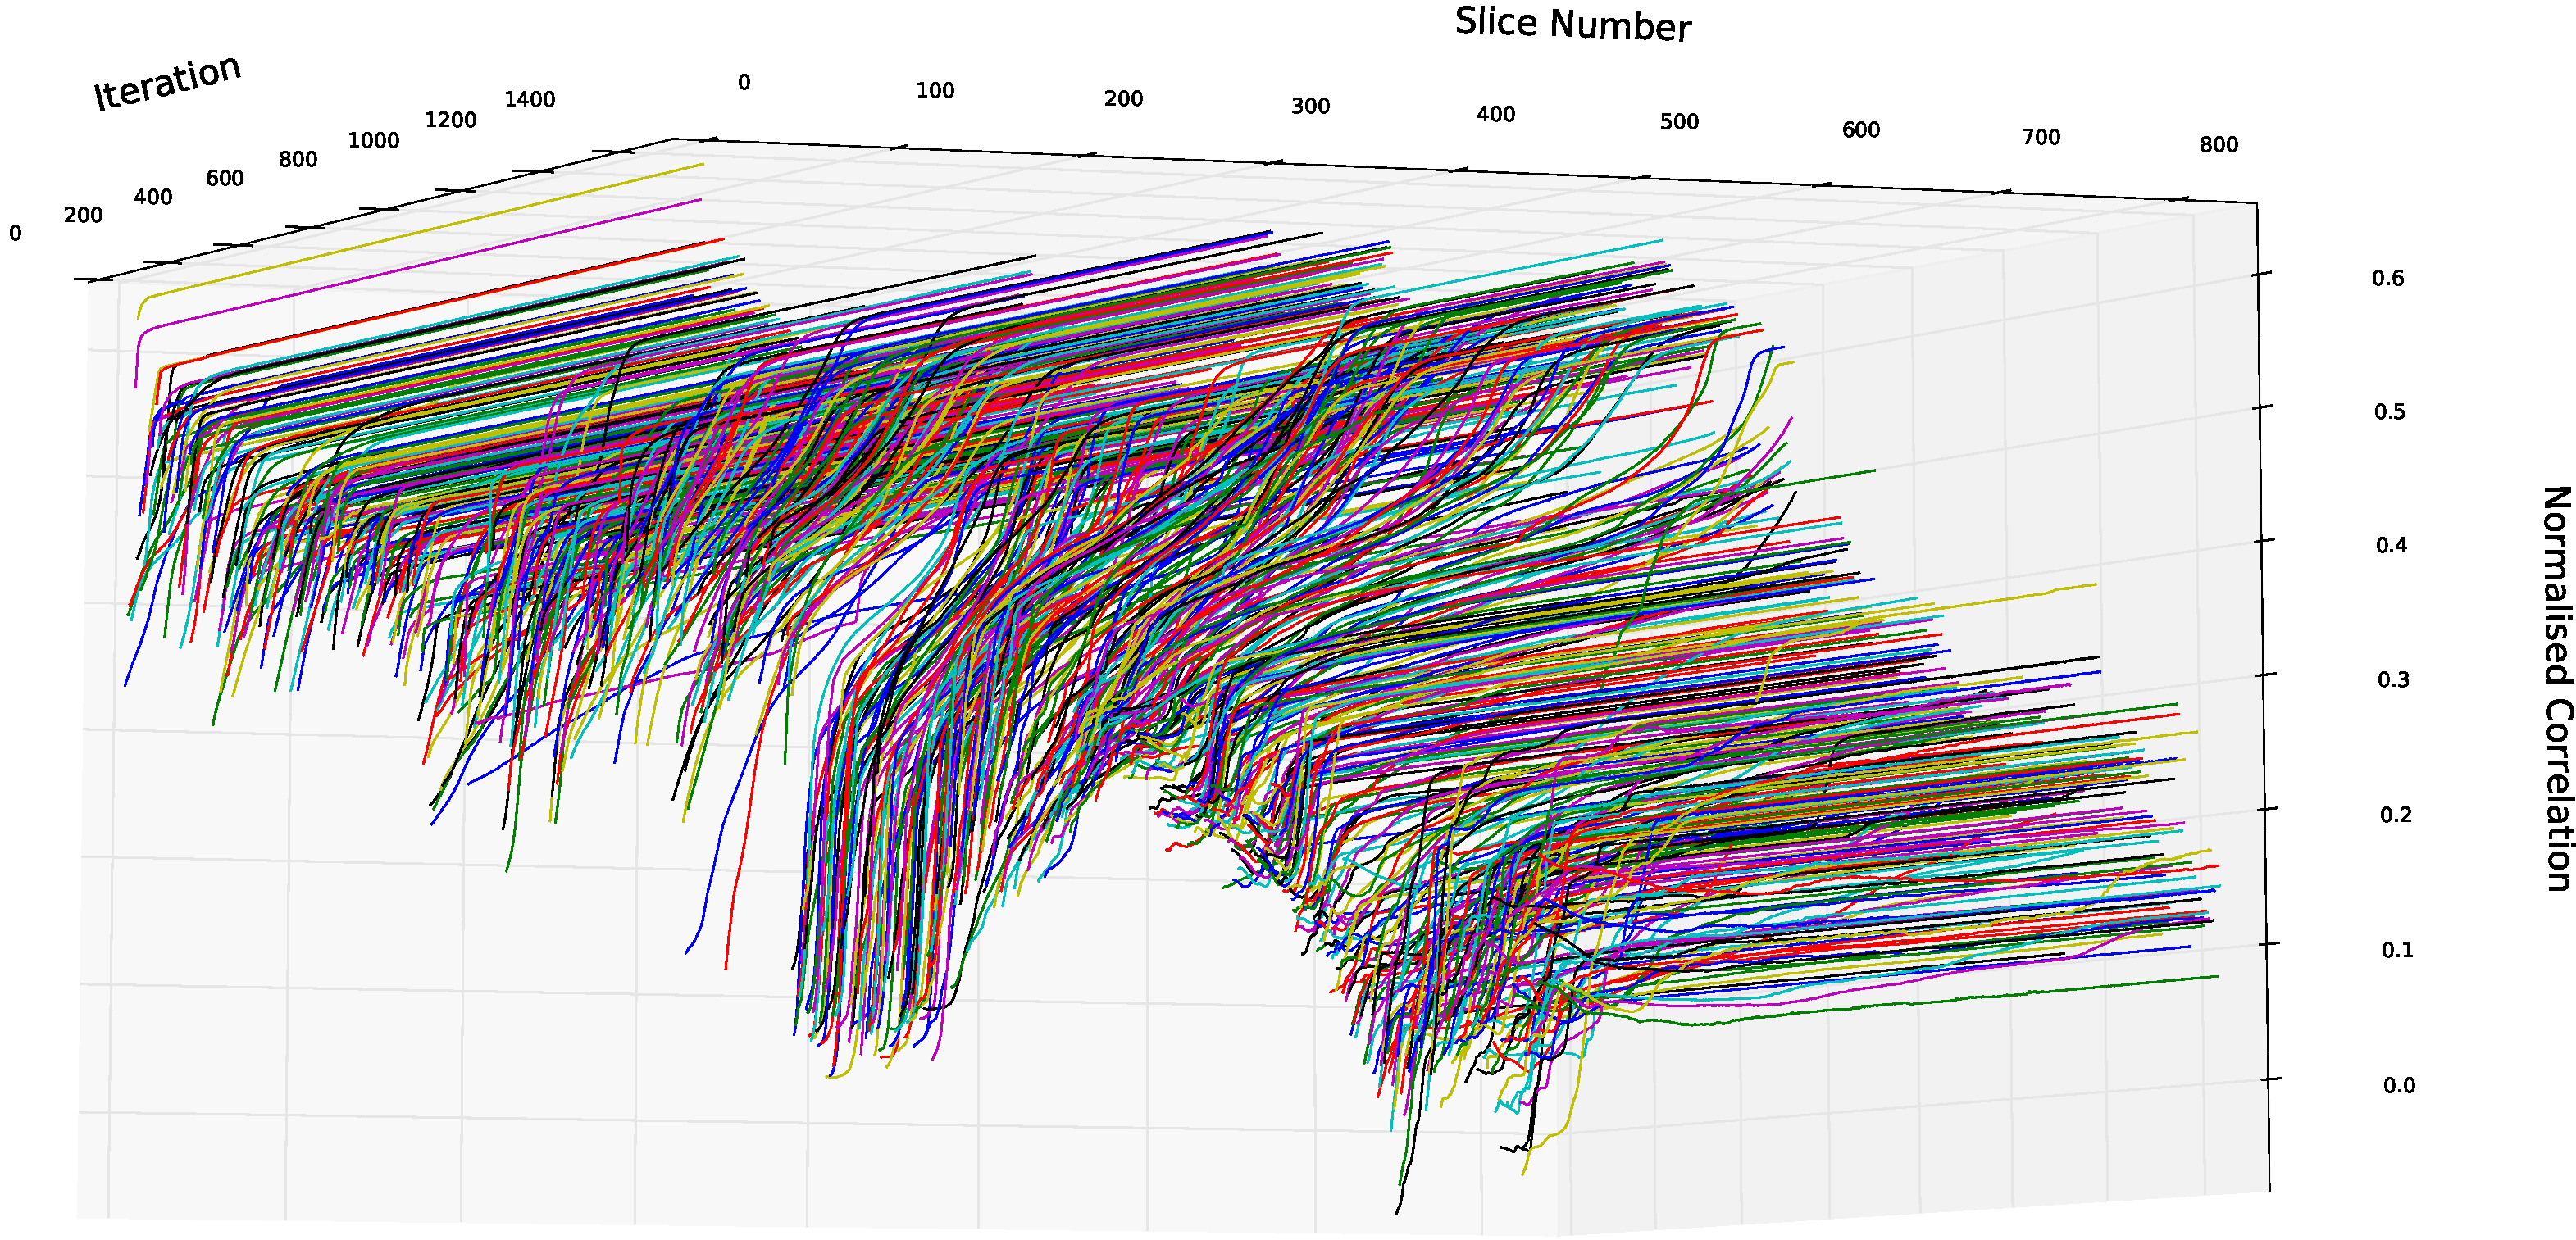
\includegraphics[width=\textheight]{Ch5/Figs/diagnostics/rigid_metric_values}
    \caption{Intermediate metric values for all slices during rigid registration.}
    \label{fig:rigid_metric_values}
  \end{sidewaysfigure}
      
  \begin{sidewaysfigure}[htbp]
    \centering
    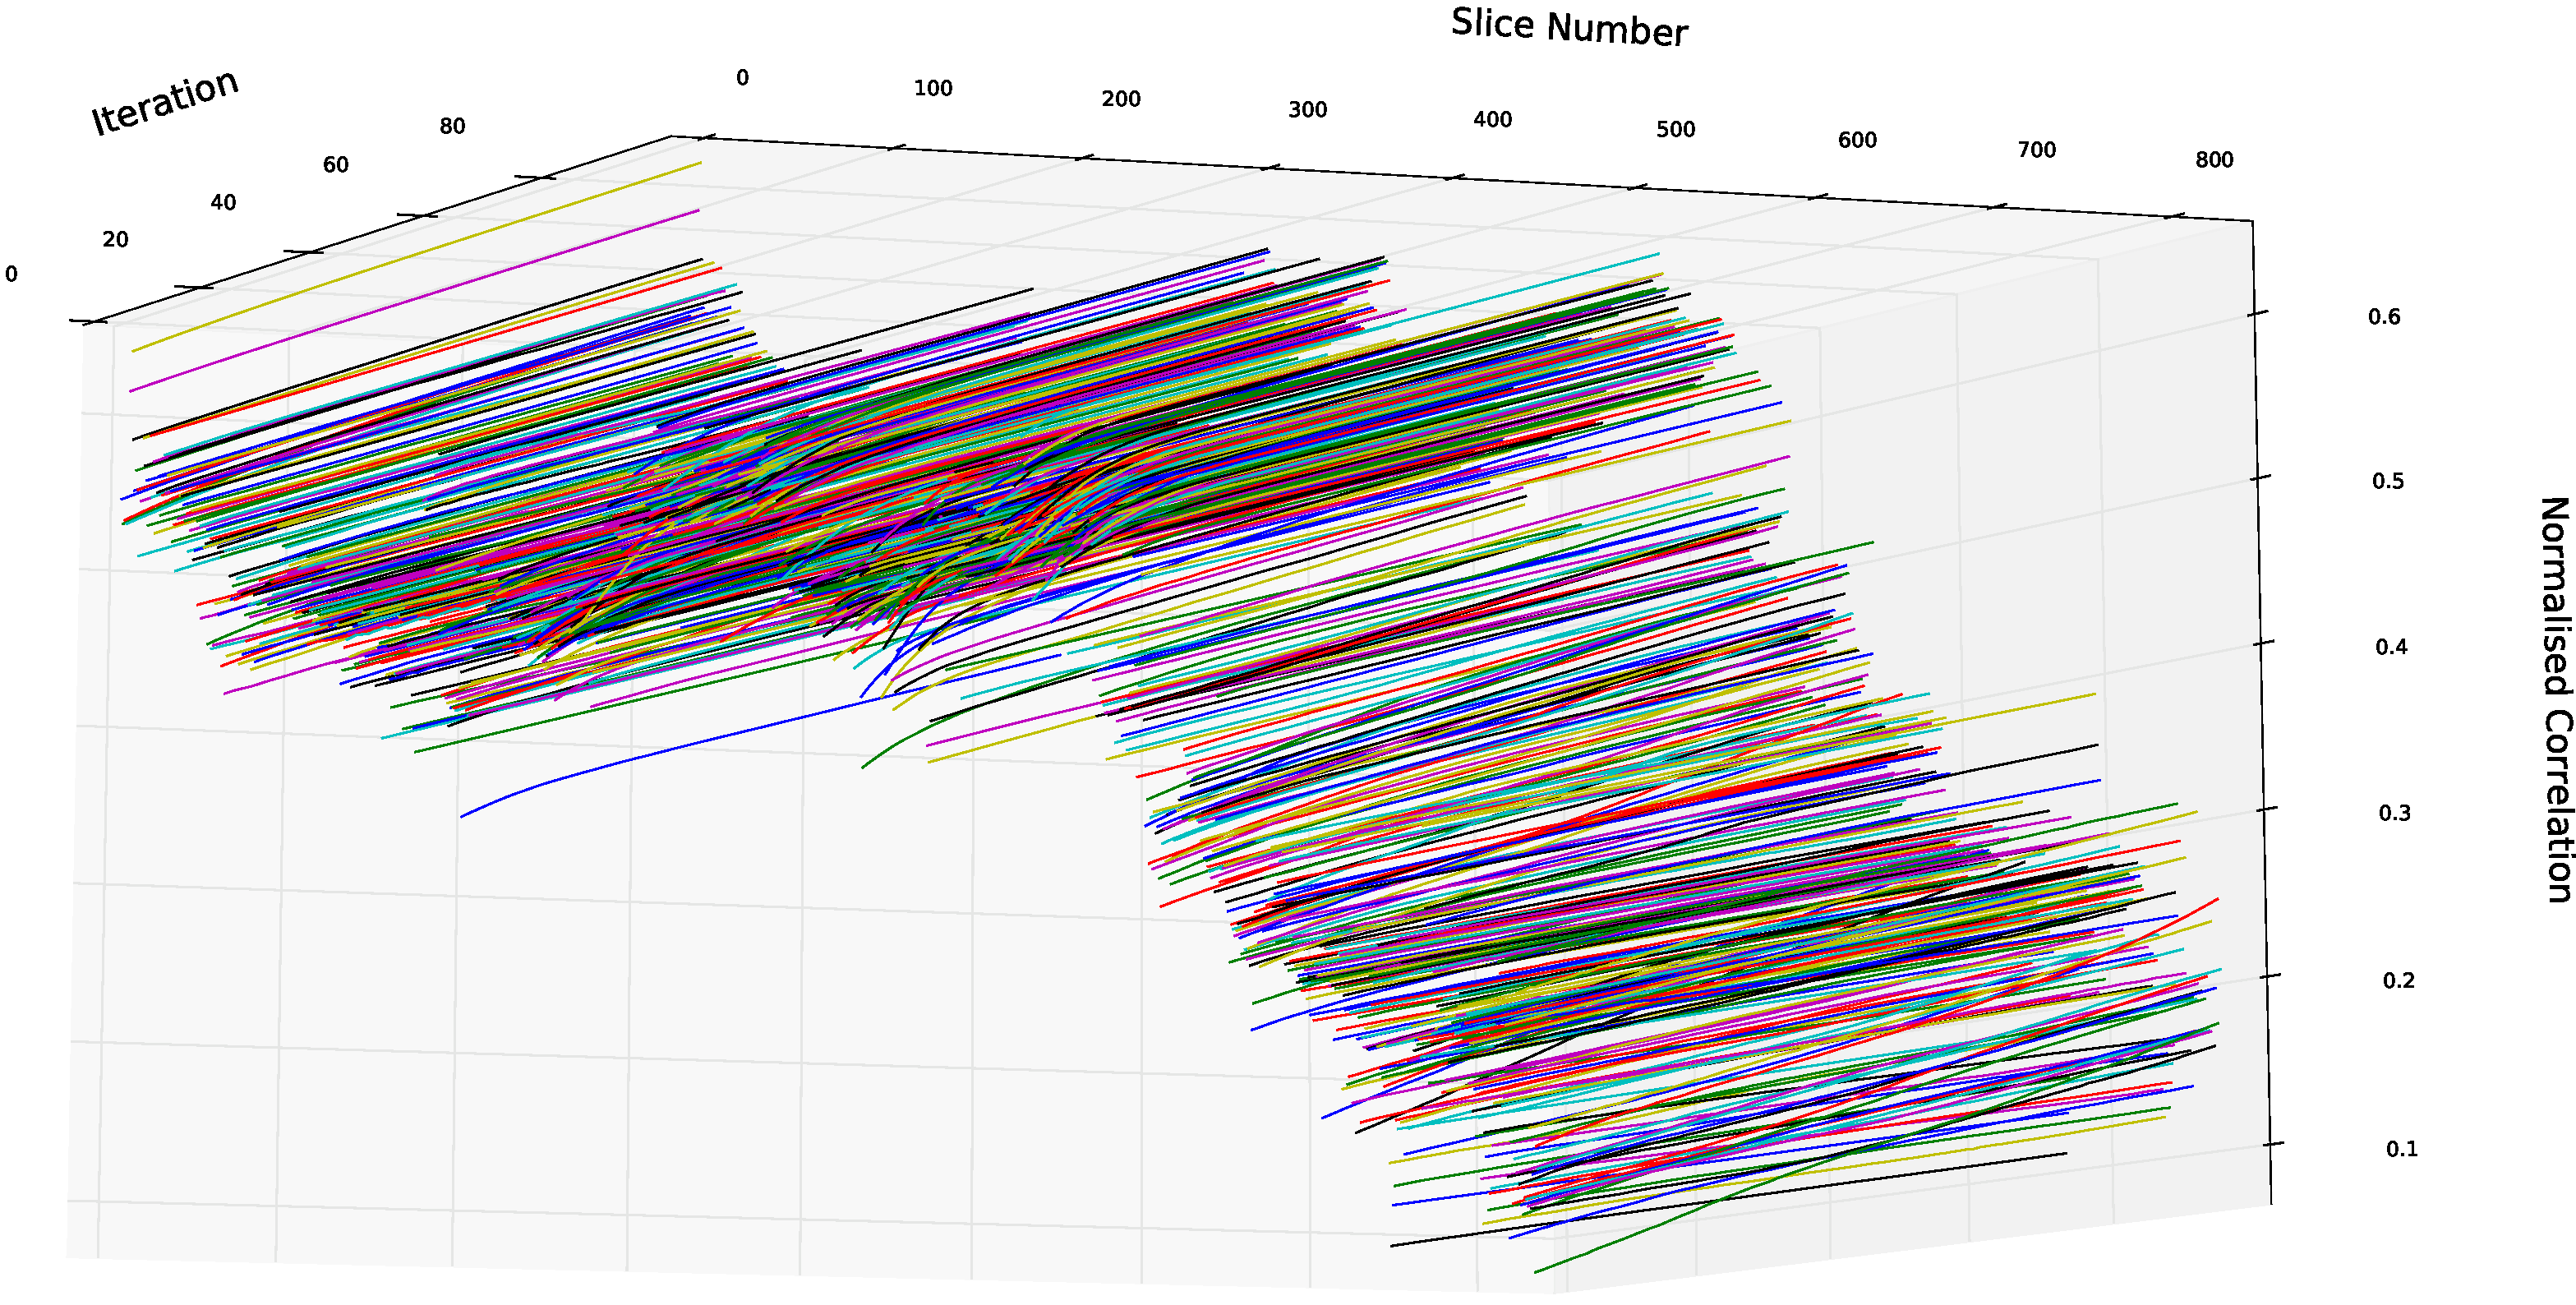
\includegraphics[width=\textheight]{Ch5/Figs/diagnostics/similarity_metric_values}
    \caption{Intermediate metric values for all slices during similarity registration.}
    \label{fig:similarity_metric_values}
  \end{sidewaysfigure}
      
  \begin{sidewaysfigure}[htbp]
    \centering
    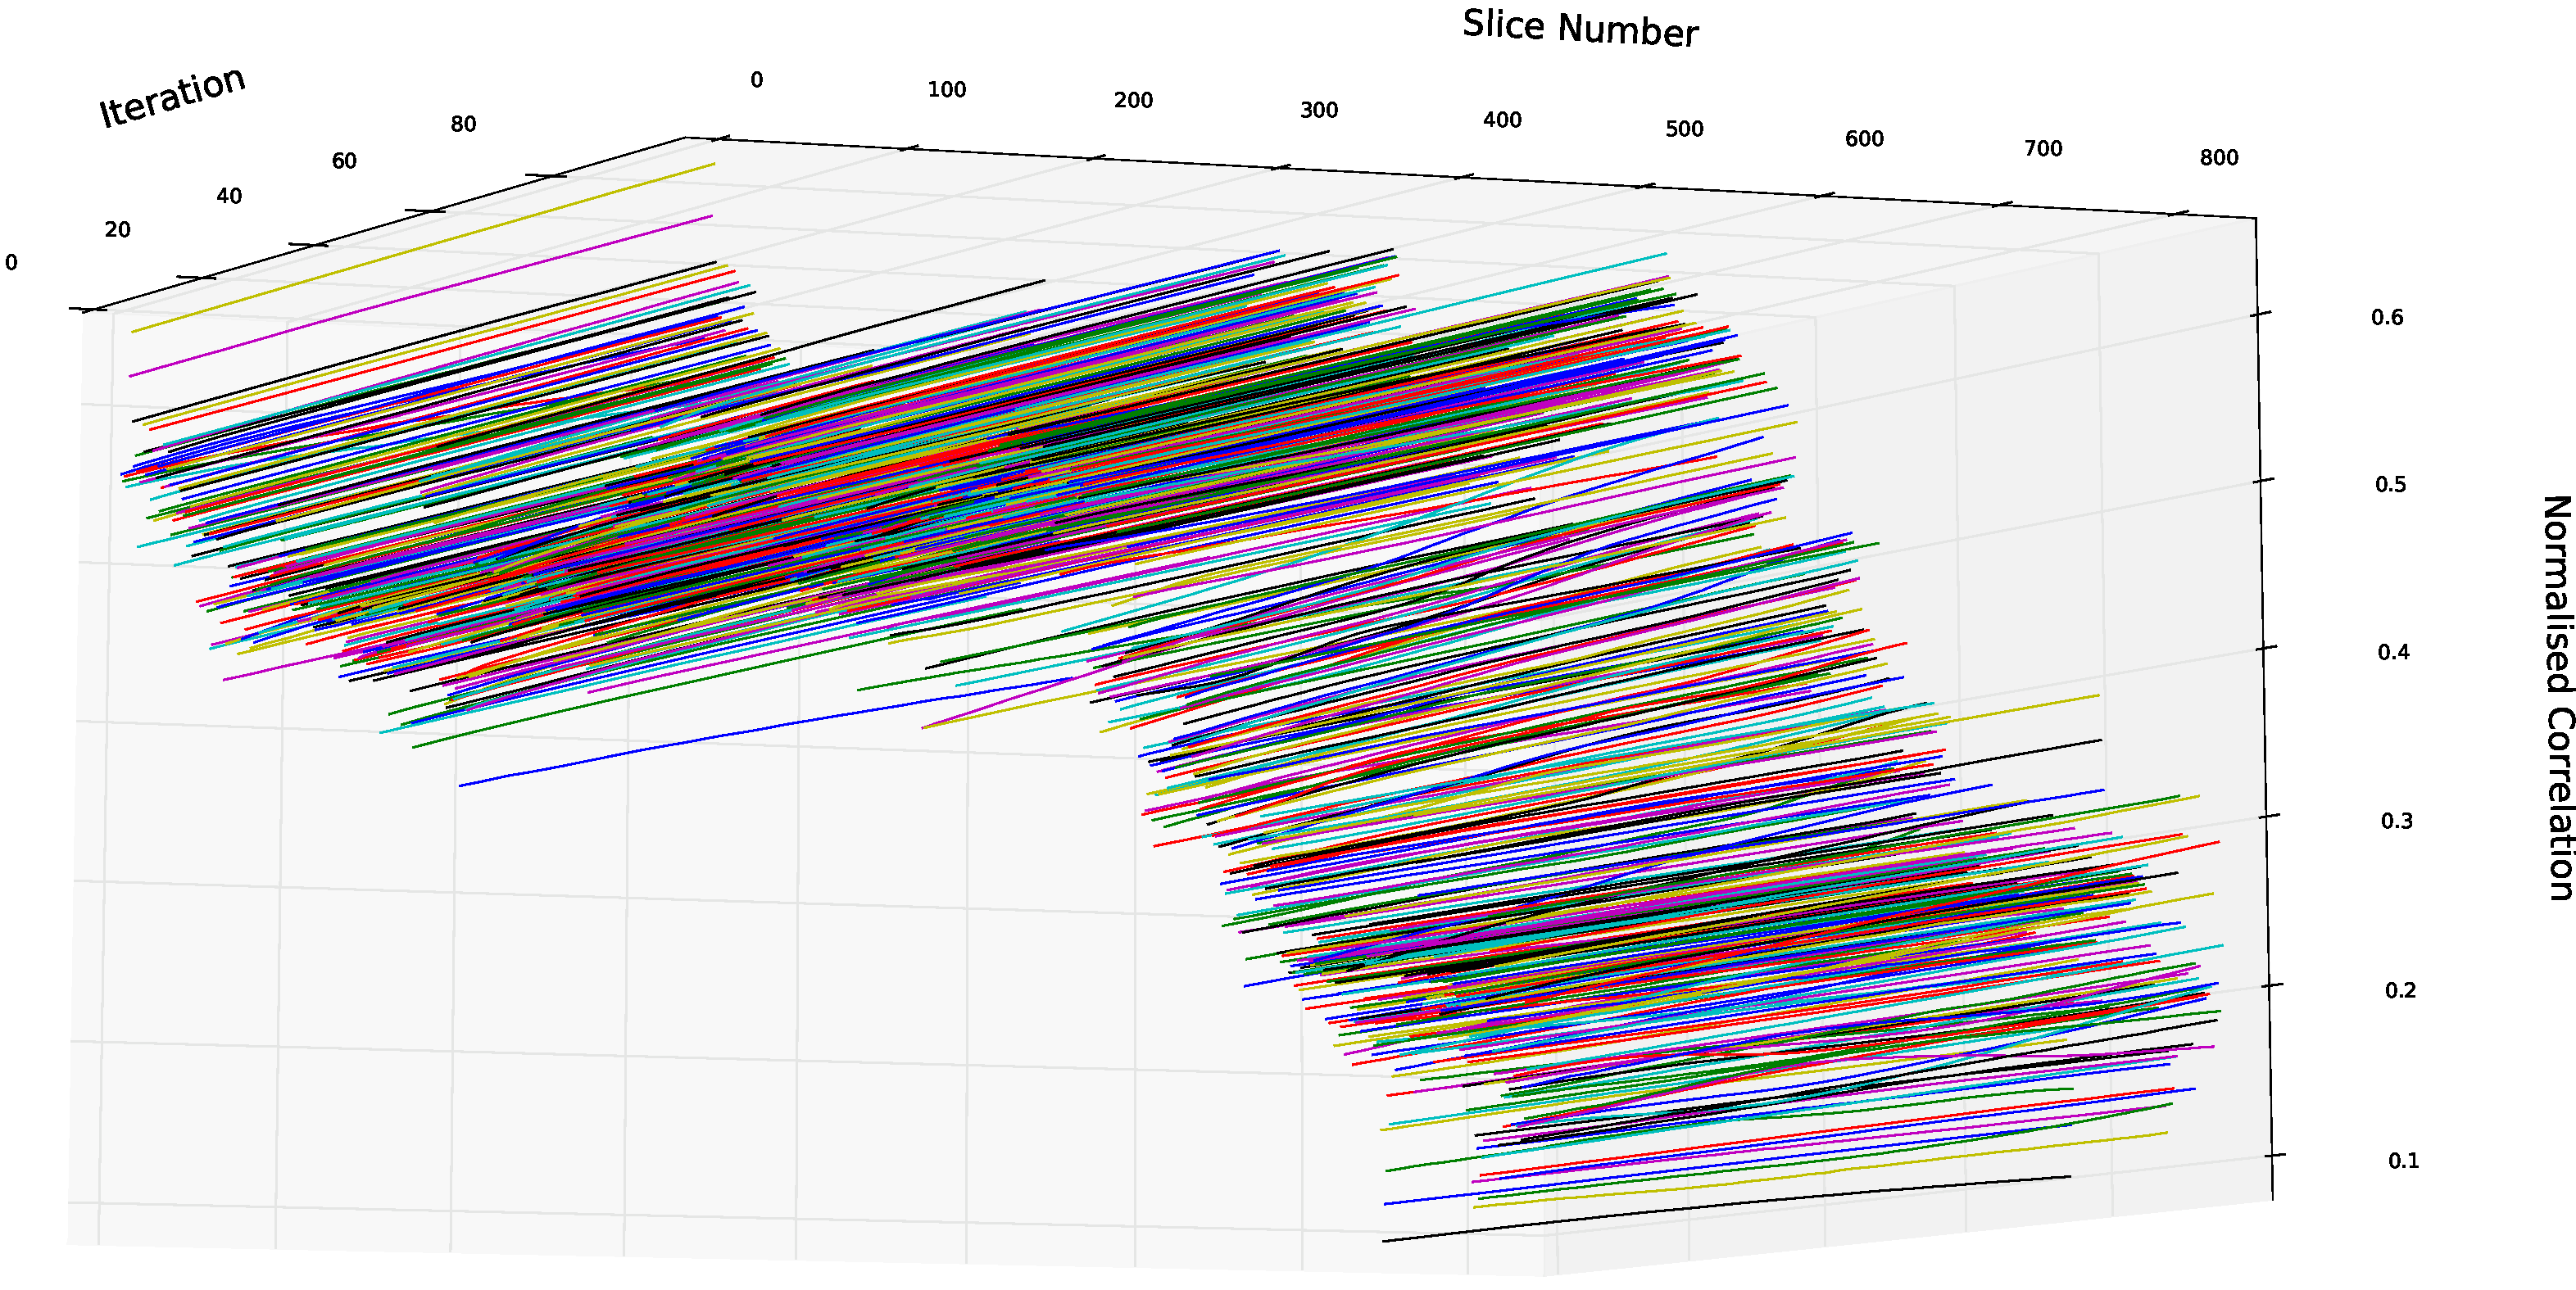
\includegraphics[width=\textheight]{Ch5/Figs/diagnostics/affine_metric_values}
    \caption{Intermediate metric values for all slices during affine registration.}
    \label{fig:affine_metric_values}
  \end{sidewaysfigure}
  
	Figures~\labelcref{fig:rigid_metric_values,fig:similarity_metric_values,fig:affine_metric_values} graph the intermediate metric values of each iteration for each slice, during the rigid, similarity and affine registrations. Each graph is viewed from below, in order to see all values clearly. Evidently, the overwhelming majority of the optimisation is done in the first rigid step, and this is reflected in the number of iterations required to reach a global optimum: 1500, as apposed to 100 for similarity and affine registrations. Nearly all curves increase smoothly and monotonically, before reaching a distinct flat maximum. In Figure~\ref{fig:rigid_metric_values} after around slice 600, where the blob-shaped artefact appears, the final metric values decrease almost linearly as the intensity of the blob increases. Slices in the region of 400-600 start from a much lower metric value, and take up to 1500 iterations to maximise; their geometric initialisations were much further from their final optimal position. Diagnostics were of critical importance here, not least to ensure that enough iterations had passed so that all slices had reached their flat optimum position.
	
  \begin{sidewaysfigure}[htbp]
    \centering
    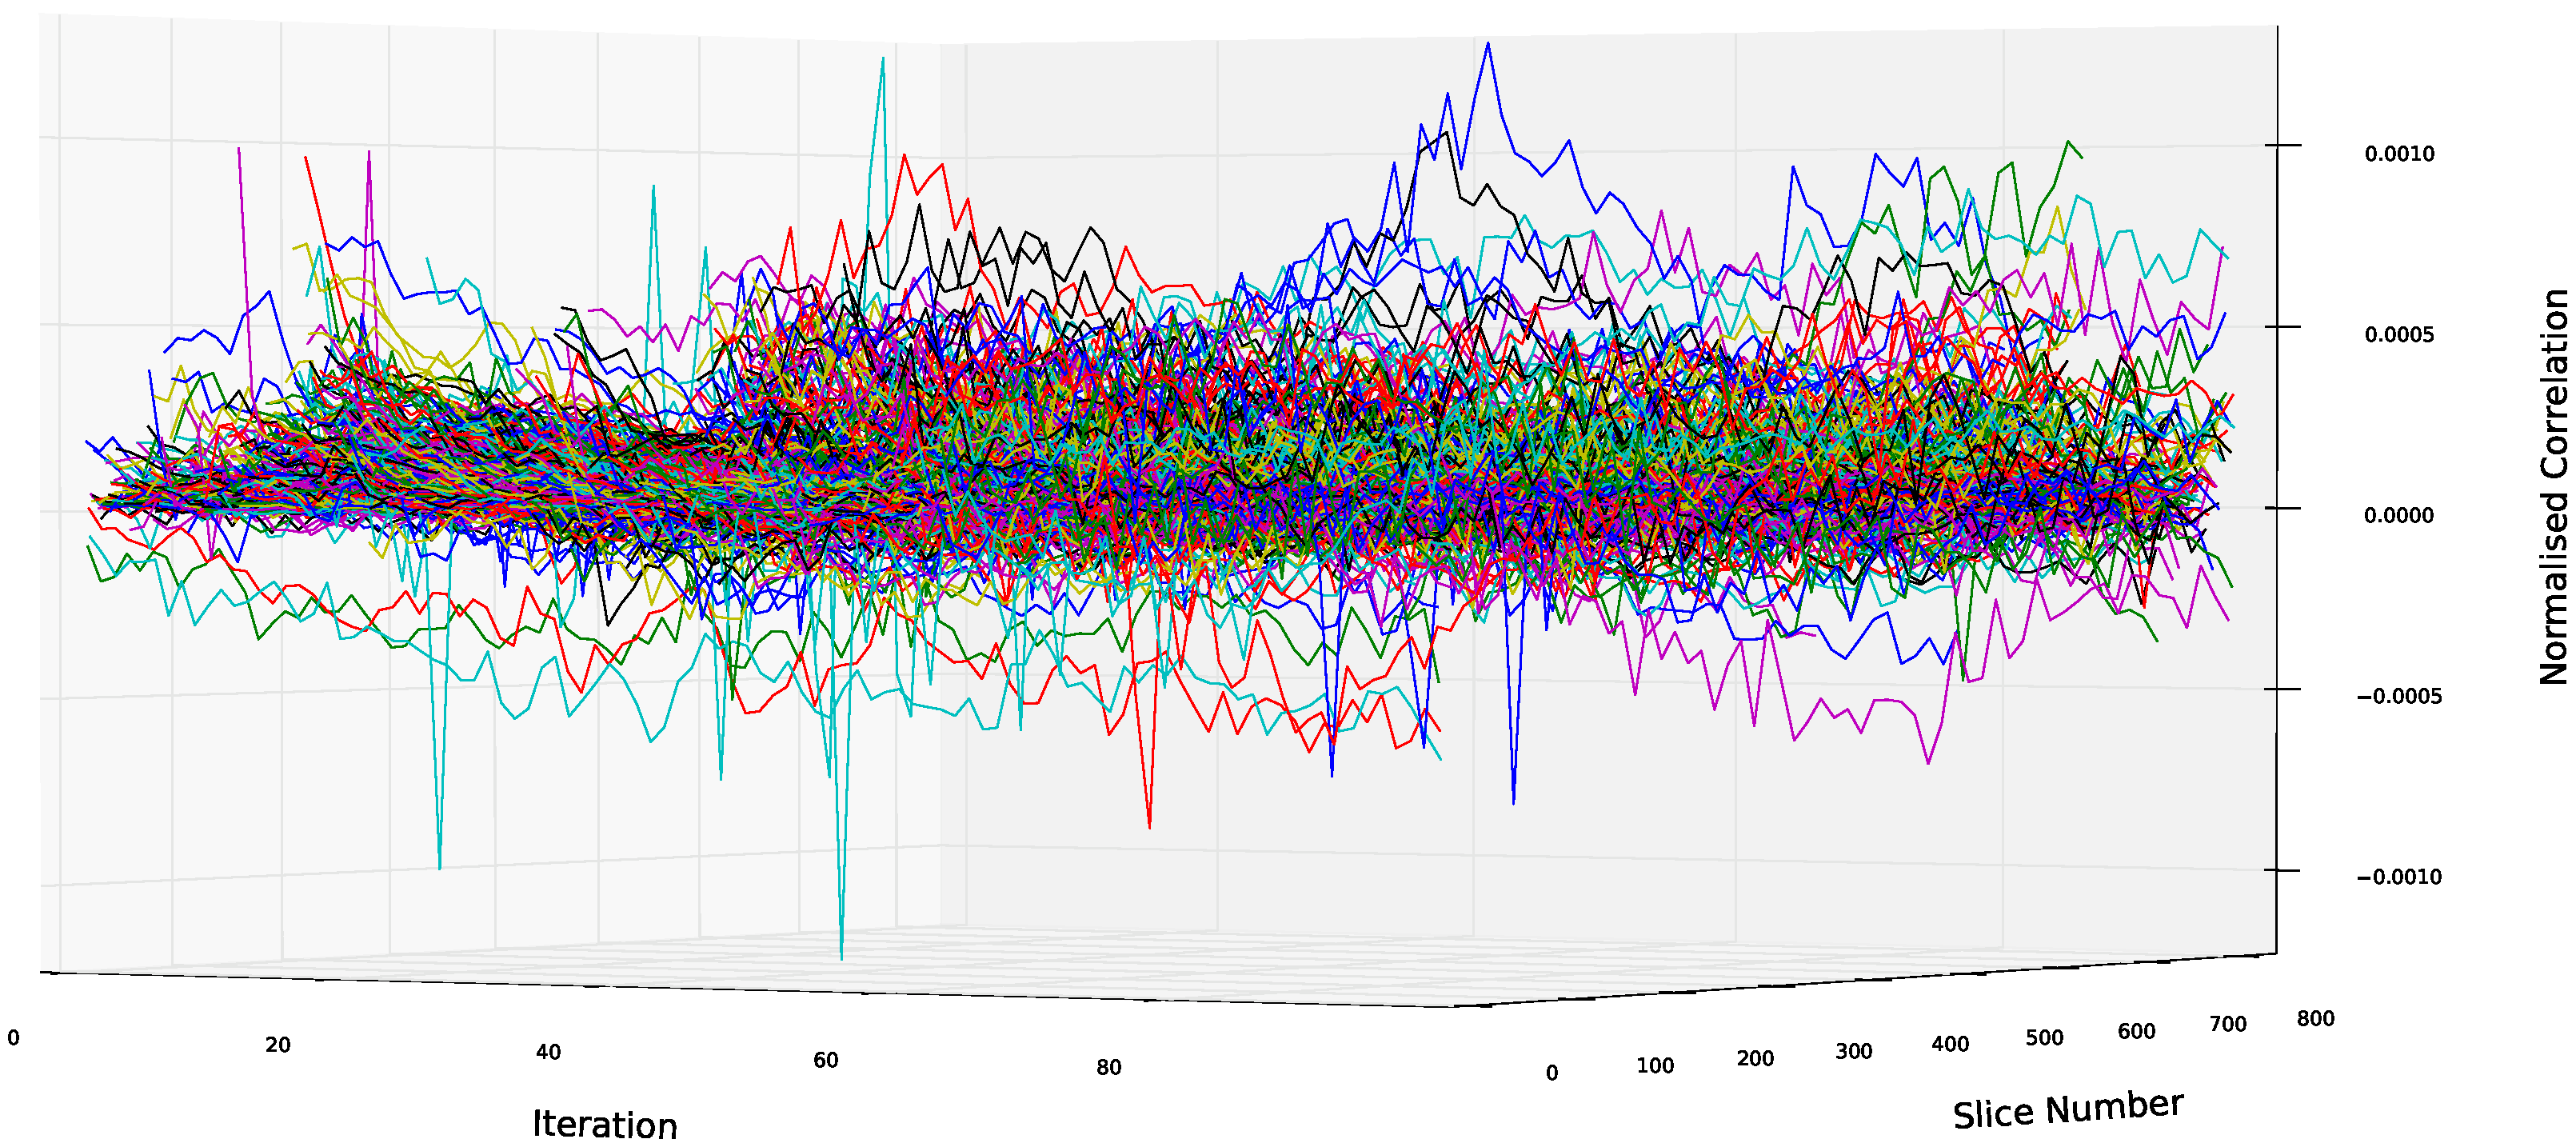
\includegraphics[width=\textheight]{Ch5/Figs/diagnostics/affine_metric_value_differences}
    \caption{Intermediate \emph{delta} metric values for all slices during affine registration i.e. the difference in metric value between subsequent iterations.}
    \label{fig:affine_metric_value_differences}
  \end{sidewaysfigure}
  
	The changes in metric value in Figure~\ref{fig:affine_metric_values} are very small compared to the range of metric values across slices. Figure~\ref{fig:affine_metric_value_differences} depicts the change in metric value upon each iteration. It is viewed from the zero plane, and demonstrates -- at least to some extent -- that these changes are weighted largely to the positive side of zero. The affine registration is a small but certain improvement upon the similarity registration.
	
  \begin{sidewaysfigure}[htbp]
    \centering
    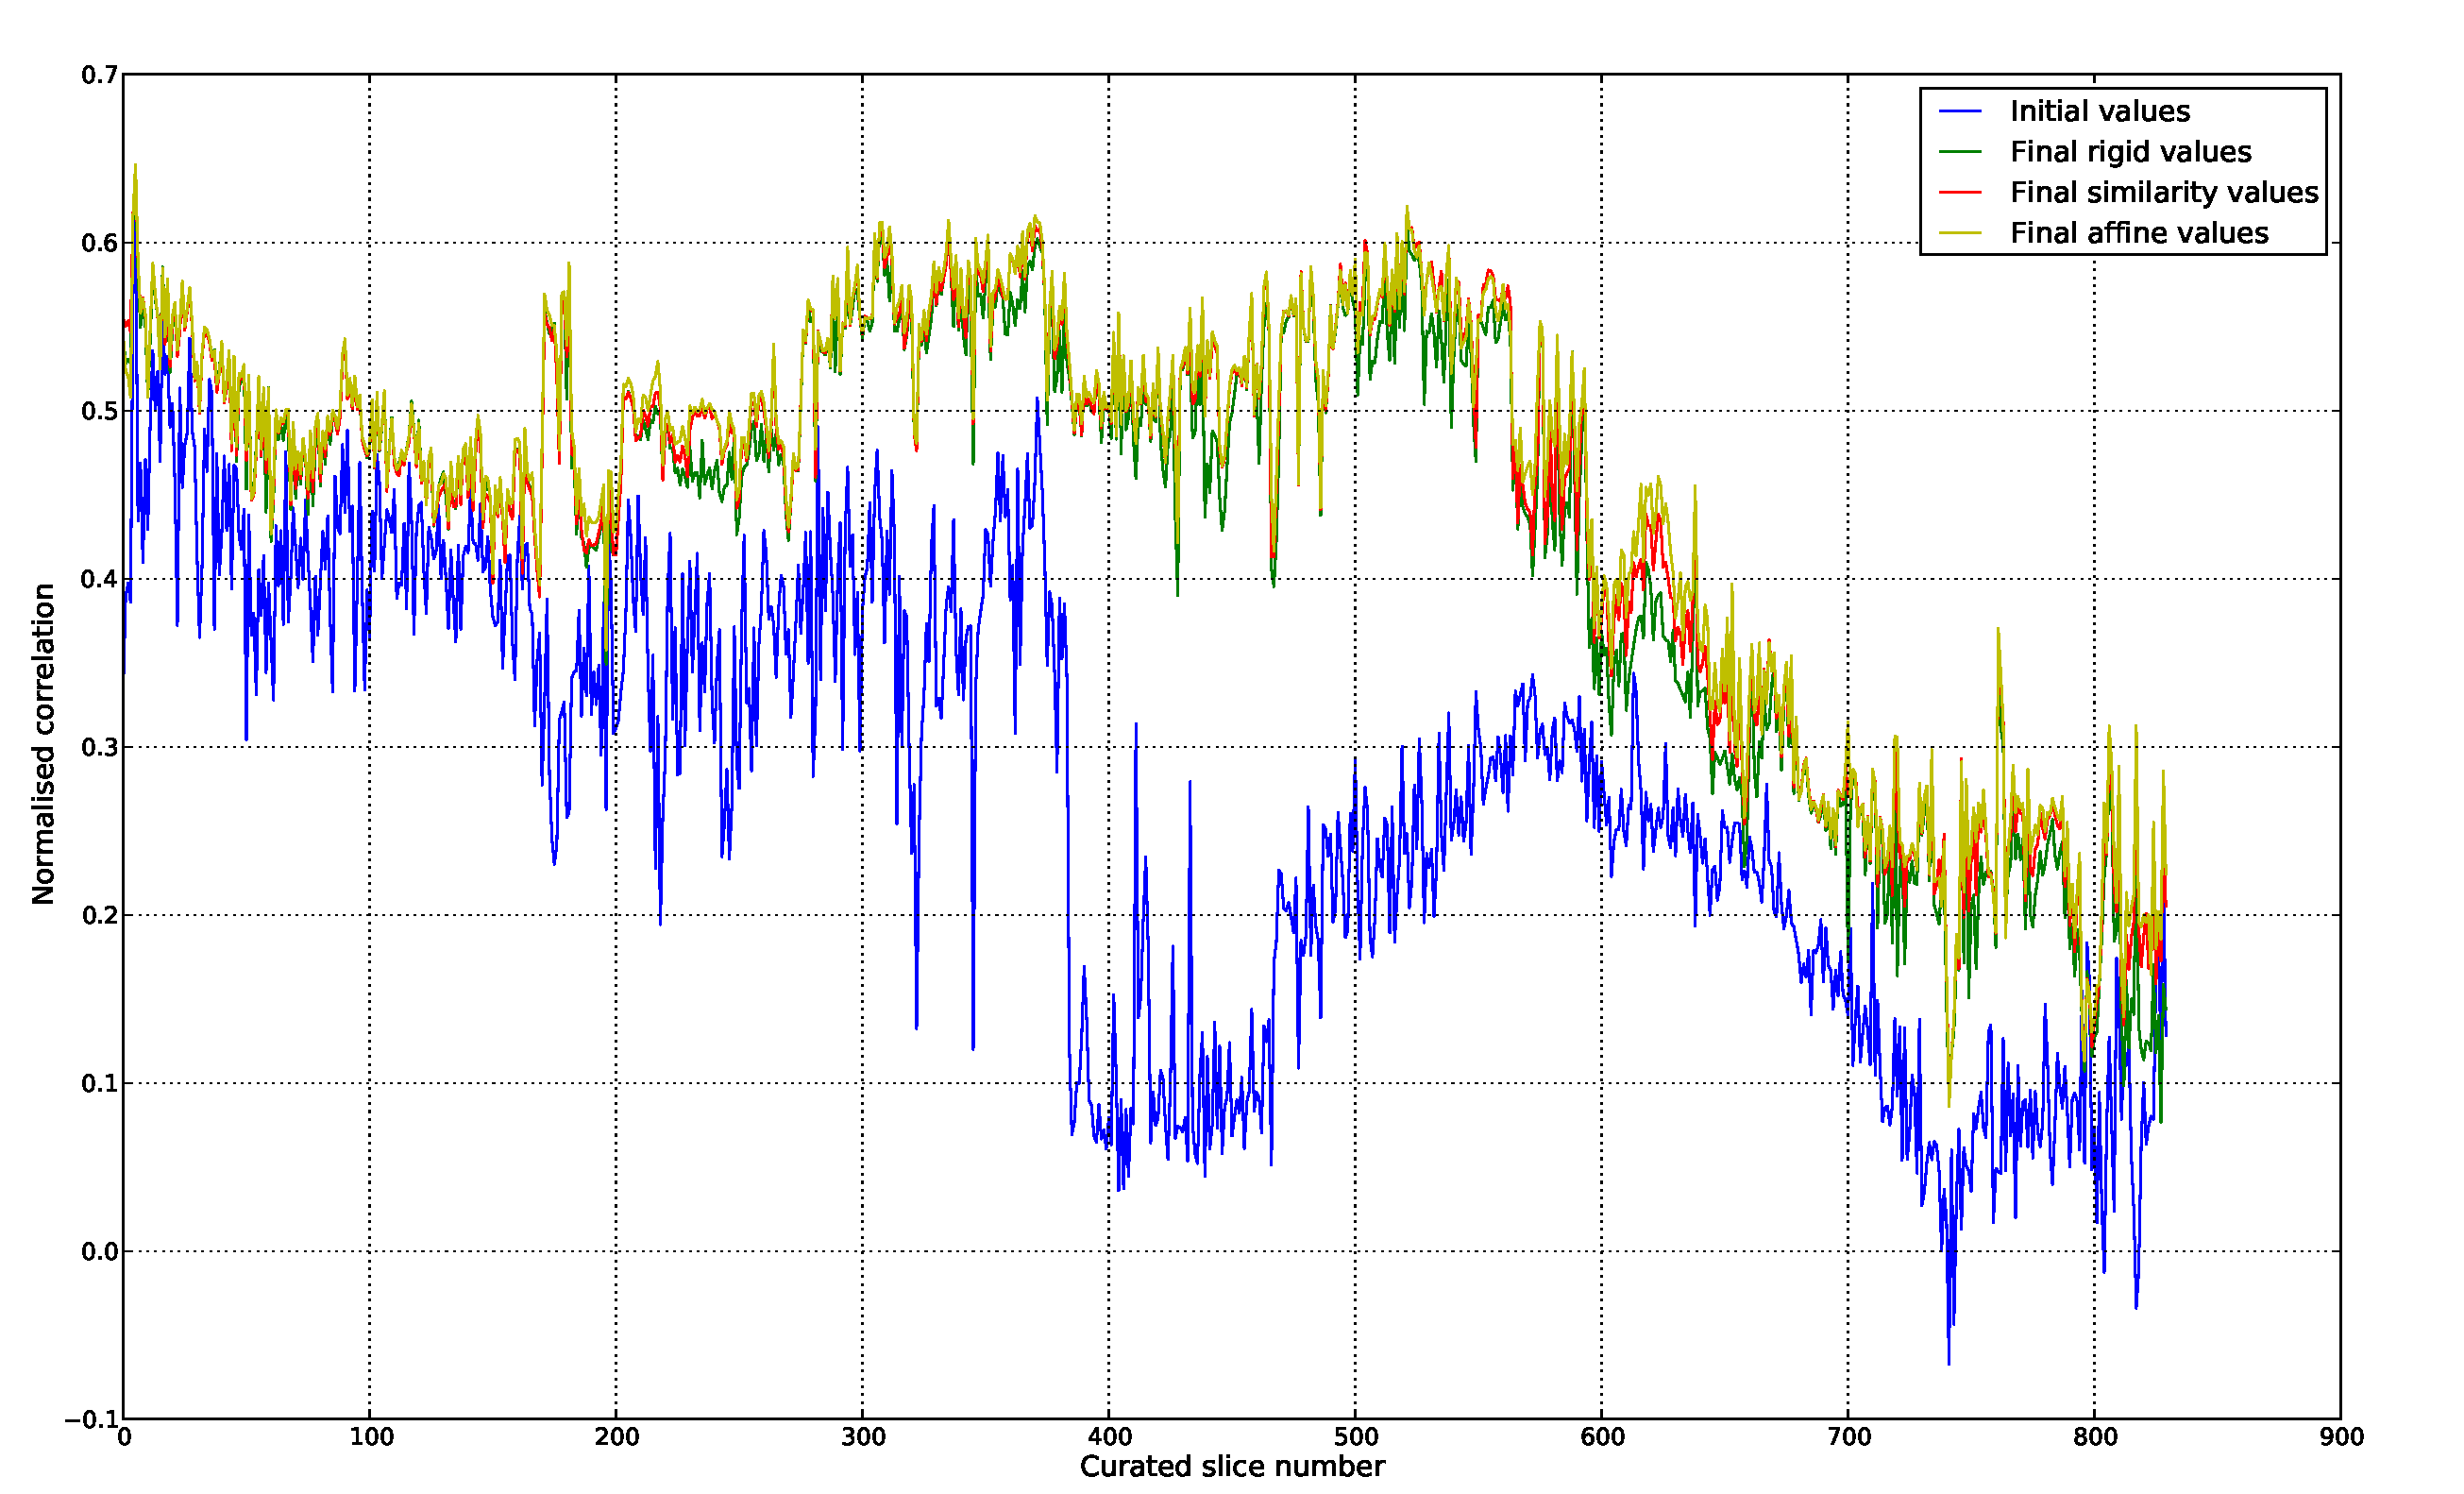
\includegraphics[width=\textheight]{Ch5/Figs/diagnostics/initial_and_final_values_comparison}
    \caption{Initial and final metric values before and after each stage of registration.}
    \label{fig:initial_and_final_values_comparison}
  \end{sidewaysfigure}
  
	Figure \ref{fig:initial_and_final_values_comparison} shows the initial metric values after geometric initialisation, and the final metric values after rigid, similarity and affine registrations. Again is it clear that each successive registration increases correlation, but the majority of improvement comes from the rigid registration. Slices from 380 to 600 were photographed at a larger angle from that of their block-face images, and this is reflected in a sharply reduced initial correlation value. From Slice 600 onwards, the blob precludes successful registration and both initial and final correlation values decline.
	
	\begin{figure}[htbp]
    \centering
    \subfigure[][]{
\includegraphics[height=0.3\textheight]{Ch5/Figs/diagnostics/fixed_progress_slice_0562_1_287.pdf}}
    \subfigure[][]{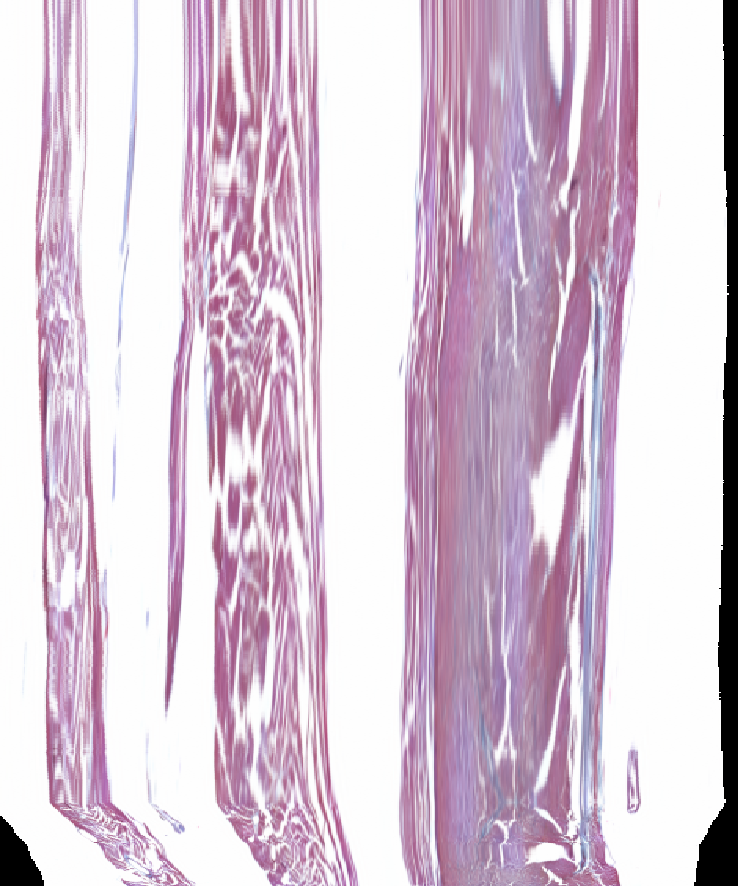
\includegraphics[height=0.3\textheight]{Ch5/Figs/diagnostics/moving_progress_slice_0562_1_287.pdf}}
    \subfigure[][]{
\includegraphics[height=0.3\textheight]{Ch5/Figs/diagnostics/fixed_progress_slice_0562_0_235.pdf}}
    \subfigure[][]{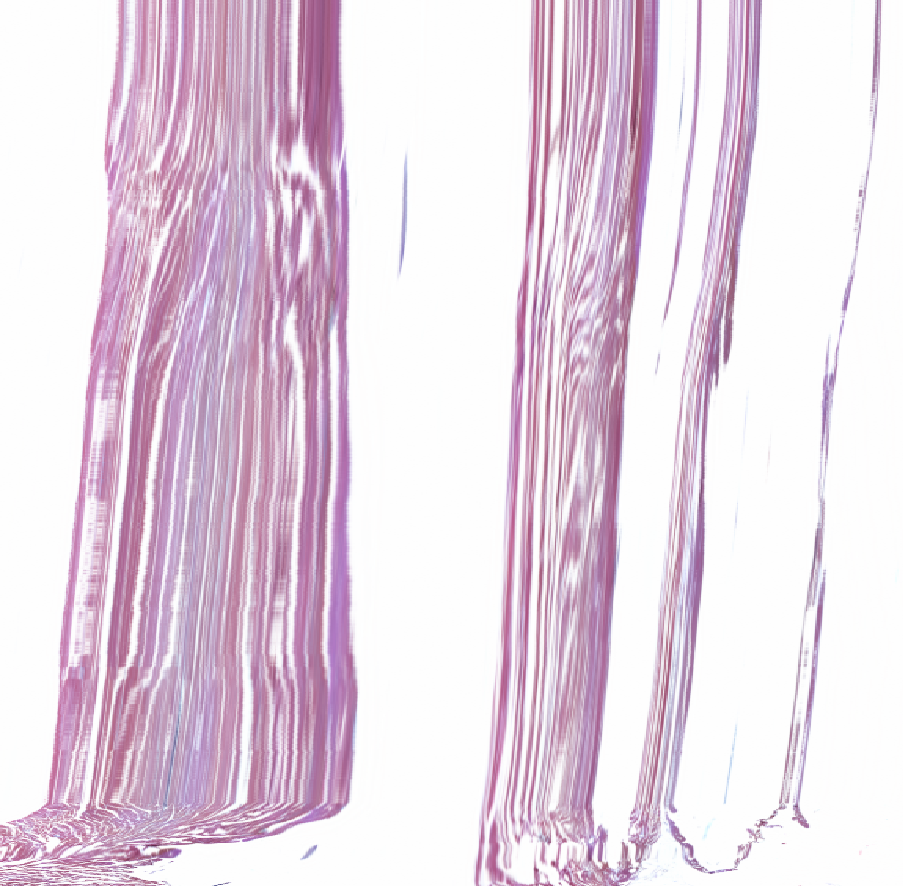
\includegraphics[height=0.3\textheight]{Ch5/Figs/diagnostics/moving_progress_slice_0562_0_235.pdf}}
    \caption{Central cross-sections of the progress volume of 1500 iterations of slice 0562, together with the fixed progress volume of the equivalent block face image.}
    \label{fig:progress_cross_sections}
  \end{figure}
      
  \begin{figure}[htbp]
    \centering
    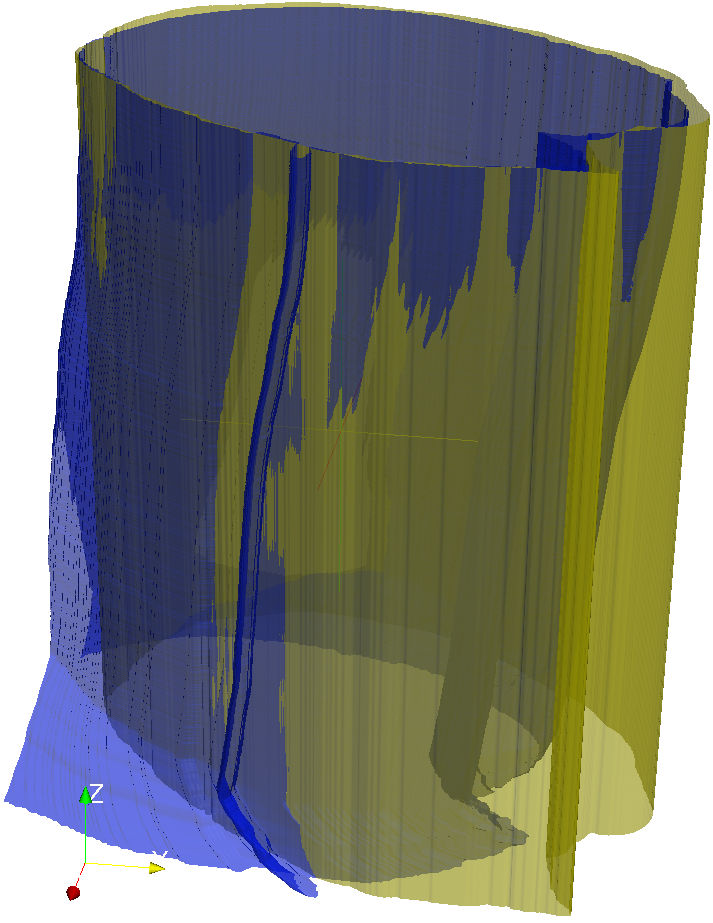
\includegraphics[width=\pagewidth]{Ch5/Figs/diagnostics/0562_contour.png}
    \caption{Contours of the progress volume of 1500 iterations of slice 0562 in blue, and of the fixed eqiuvalent block face image in yellow. Isosurfaces were extracted from volumes built from manual segmentations of both the block face and the slice image.}
    \label{fig:progress_contour}
  \end{figure}
      
  \begin{figure}[p]
    \centering
    \subfigure[][]{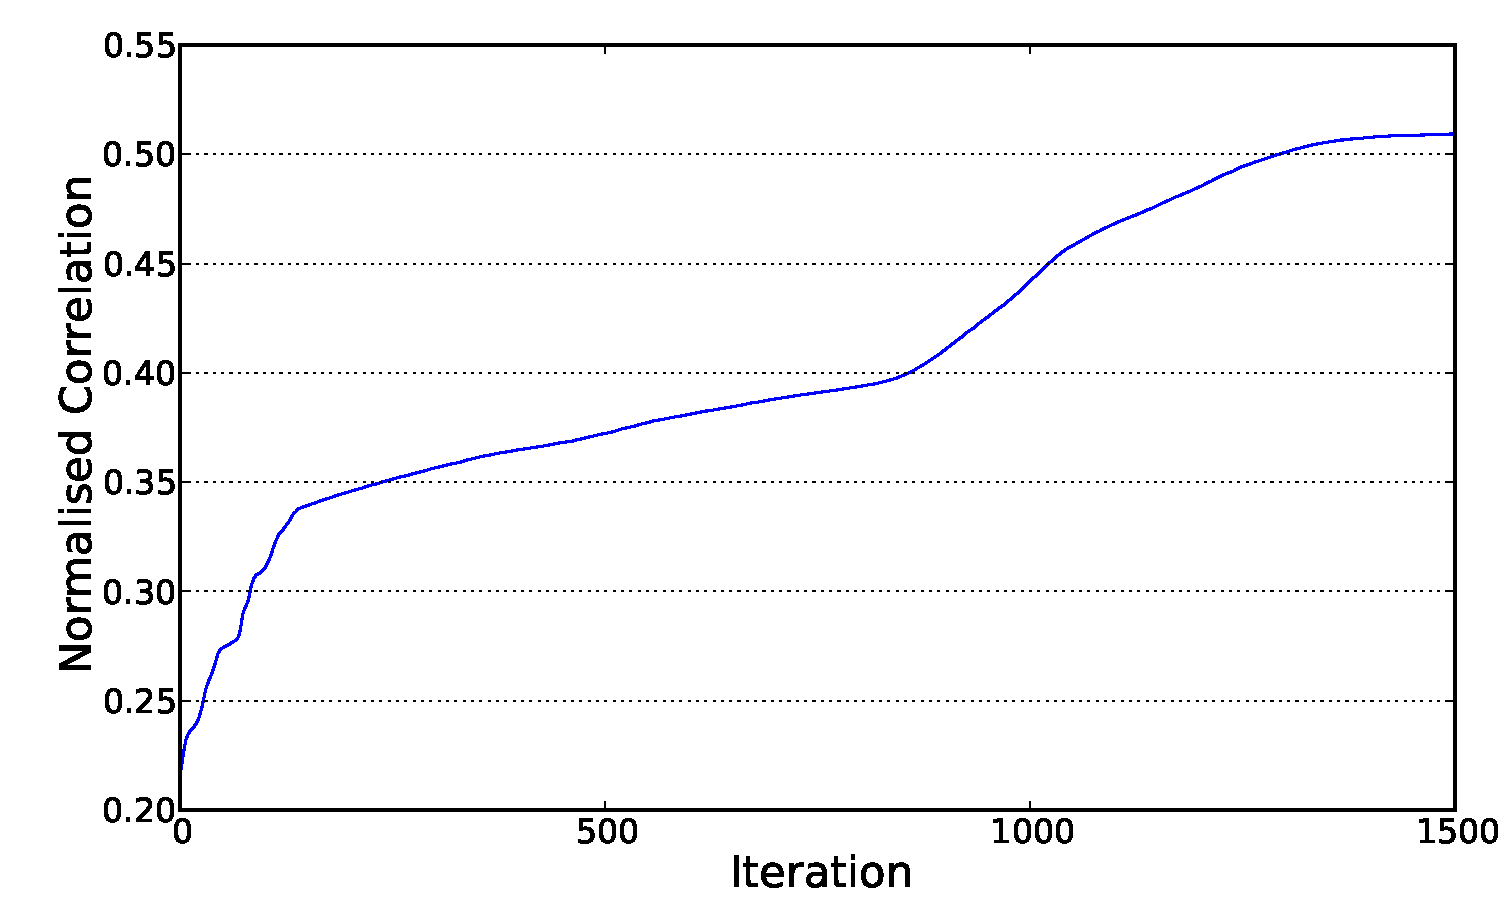
\includegraphics[width=0.9\pagewidth]{Ch5/Figs/diagnostics/0562_correlation}}
    \subfigure[][]{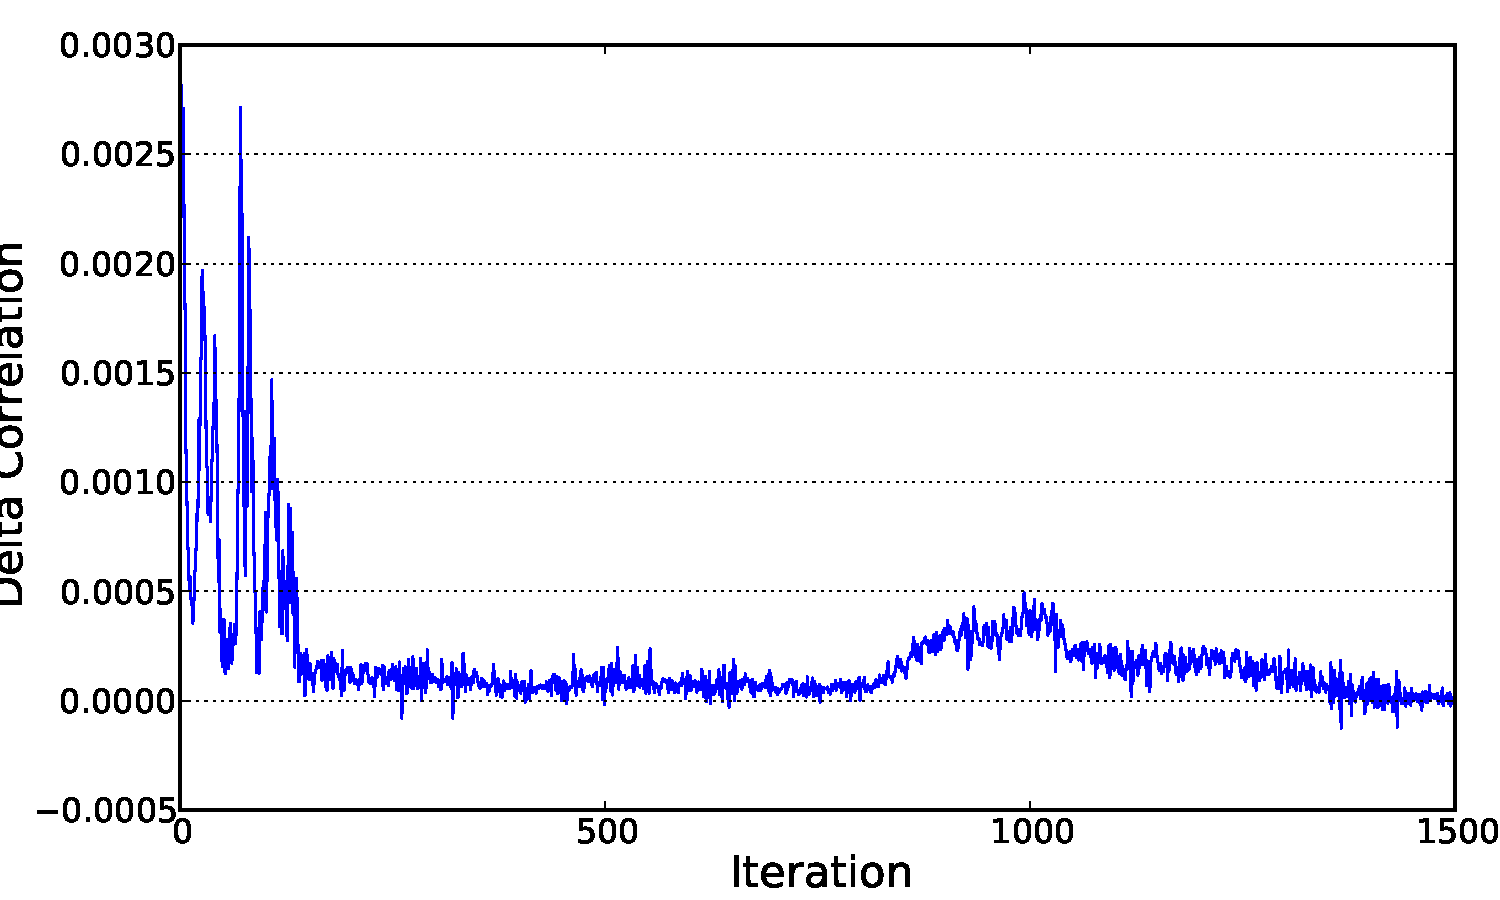
\includegraphics[width=0.9\pagewidth]{Ch5/Figs/diagnostics/0562_delta_correlation}}
    \caption{Metric values and delta metric values during the rigid registration of slice 0562.}
    \label{fig:0562_correlation}
  \end{figure}
	
	Figures~\labelcref{fig:progress_cross_sections,fig:progress_contour,fig:0562_correlation} showcase the diagnostics for a single representative slice during rigid registration. Figures~\labelcref{fig:progress_cross_sections,fig:progress_contour} are representations of the progress volume: a stack of the same 0562 image, transformed by the updating rigid transform at each of the 1500 steps in the registration. The rotation angle is quickly optimised in the first 100 iterations at the base. A flatter, slower translational optimisation ensues, which finally reaches a stationary minimum over the last iterations at the top. The top of Figure~\ref{fig:progress_contour} shows a very close fit compared with the starting point. The distinct phases of the registration are mirrored in the metric values of Figure~\ref{fig:0562_correlation}. The rapid rotational phase is seen again in the first 100 steps, with the largest metric gradients of the whole registration. A smooth, monotonic translational phase for the next 700 iterations accelerates as it gets close to the optimum, until coming to rest at around 1450 iterations.
	
	% initialisation figure
	\begin{sidewaysfigure}[htbp]
	  \centering
	  \subfigure[][]{
\includegraphics[height=0.31\textheight]{Ch5/Figs/geometric_0_235}}
	  \subfigure[][]{
\includegraphics[height=0.31\textheight]{Ch5/Figs/geometric_1_287}}
	  \caption{Central cross-sections of the slice image stack before registration. \textbf{(a)} is perpendicular to the x-axis, and \textbf{(b)} to the y-axis.}
	  \label{fig:geometric_initialisation}
	\end{sidewaysfigure}

	% x slices
	\begin{figure}[htbp]
	  \centering
	  \subfigure[][]{
\includegraphics[height=0.31\textheight]{Ch5/Figs/rigid_0_235}}
	  \subfigure[][]{
\includegraphics[height=0.31\textheight]{Ch5/Figs/size_0_235}}
	  \subfigure[][]{
\includegraphics[height=0.31\textheight]{Ch5/Figs/affine_0_235}}
	  \caption{Cross-sections of the rigid, similarity and affine volumes perpendicular to the x-axis.}
	  \label{fig:hires_0_235}
	\end{figure}

	% y slices
	\begin{figure}[htbp]
	  \centering
	  \subfigure[][]{
\includegraphics[height=0.31\textheight]{Ch5/Figs/rigid_1_287}}
	  \subfigure[][]{
\includegraphics[height=0.31\textheight]{Ch5/Figs/size_1_287}}
	  \subfigure[][]{
\includegraphics[height=0.31\textheight]{Ch5/Figs/affine_1_287}}
	  \caption{Cross-sections of the rigid, similarity and affine volumes perpendicular to the y-axis.}
	  \label{fig:hires_1_287}
	\end{figure}

	Central cross-sections of the geometrically initialised volume before registration are shown in Figure~\ref{fig:geometric_initialisation}, and cross-sections after each stage of the registration are shown in Figures~\labelcref{fig:hires_0_235,fig:hires_1_287}. The incoherent volumes in Figure~\ref{fig:geometric_initialisation} are brought into alignment by rigid registration, with small incremental improvements from similarity and affine. The improvements in the later stages are most evident at the extremities to the left and right of the figures, where the effects of small changes in parameters are most evident; edges are smoother, tissue microstructure is more clearly discerned and large displacements are mostly removed. Discontinuities in intensity between block face images, visible in Figure~\ref{fig:LoRes_cross_sections}, are mirrored in the registration. It is also clear that registration has failed from slice 600 upwards.
	
	% geometric contours
	\begin{sidewaysfigure}[p]
	  \centering
	  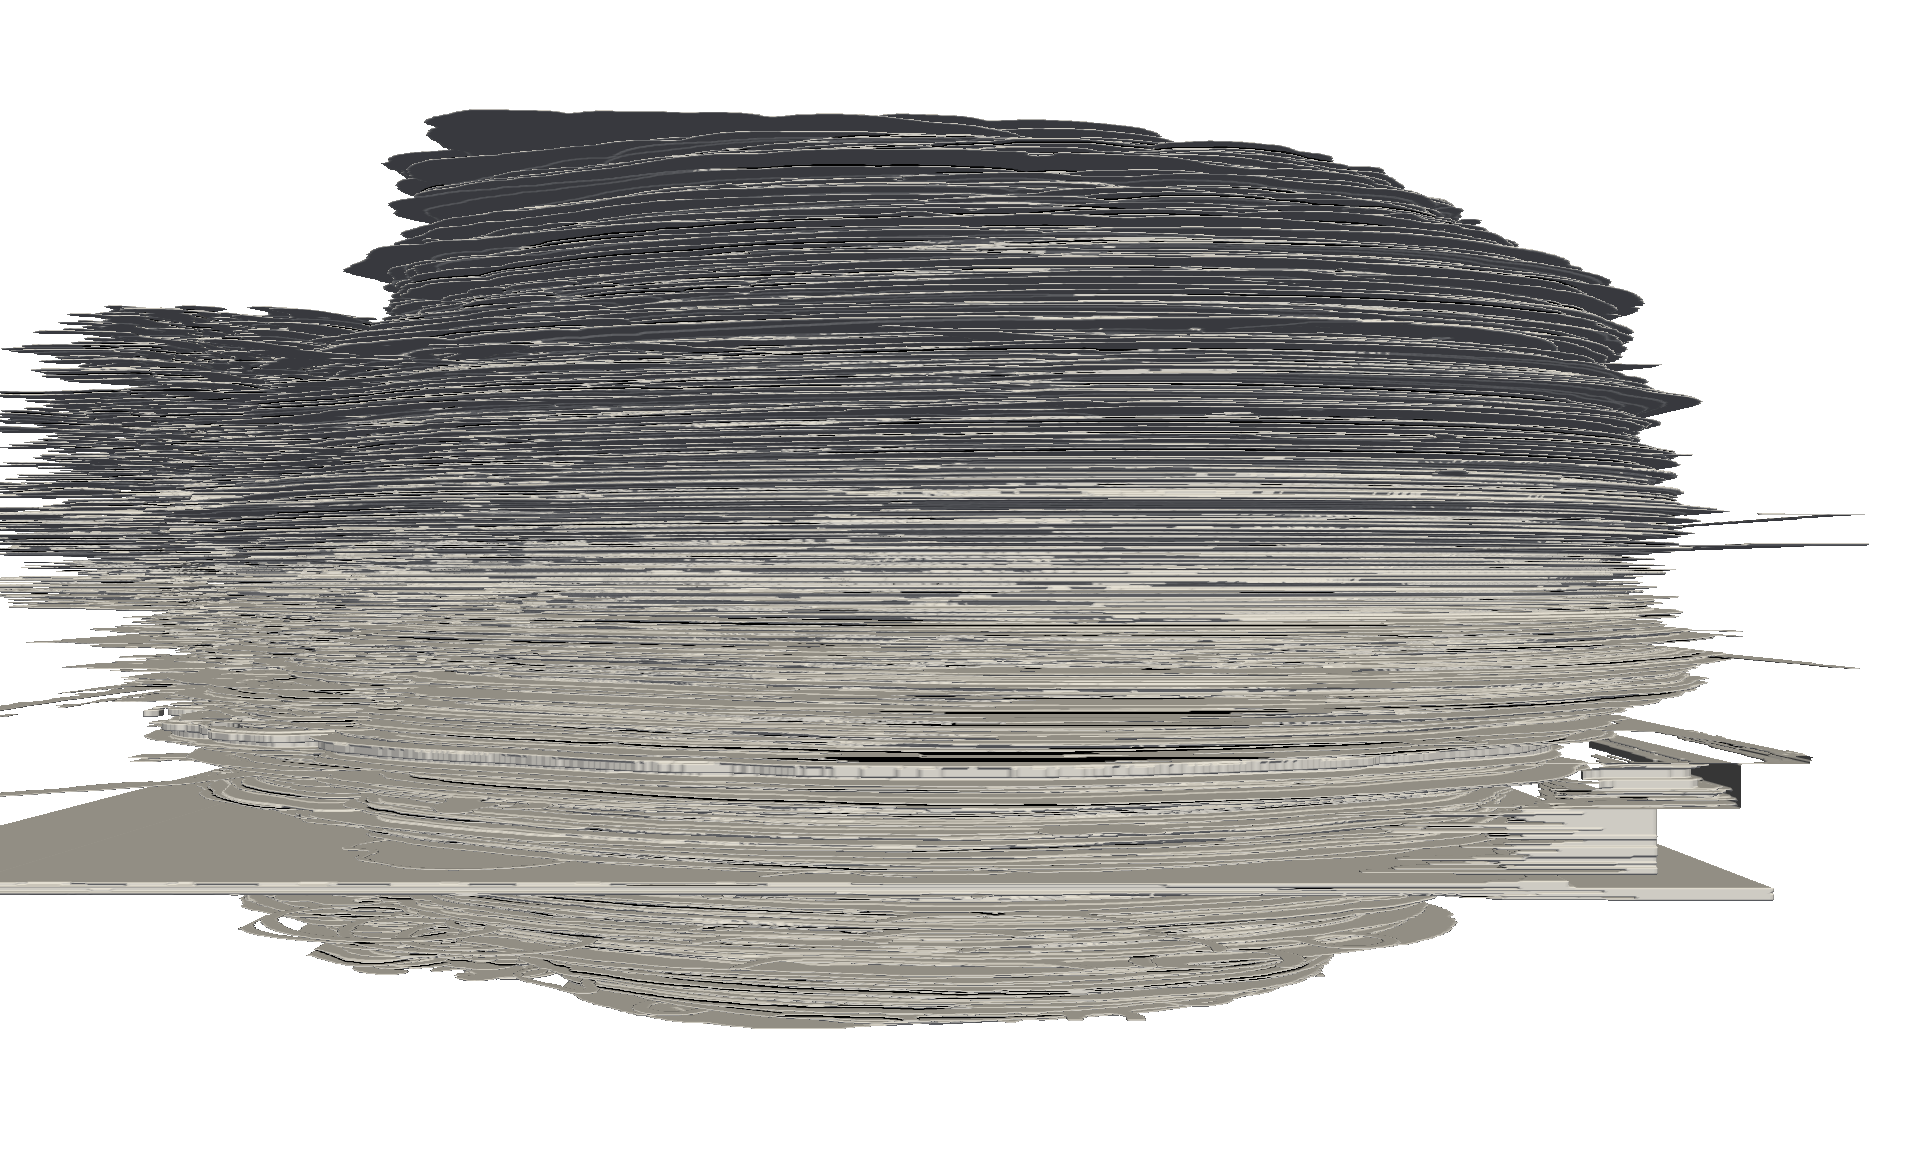
\includegraphics[width=0.9\textheight]{Ch6/Figs/Rat28/contours/whole_positive_x_geometric}
	  \caption{Geometrically initialised slice volume, viewed along the positive x direction.}
	  \label{fig:positive_x_geometric_contour}
	\end{sidewaysfigure}

	\begin{sidewaysfigure}[p]
	  \centering
	  \includegraphics[width=0.9\textheight]{Ch6/Figs/Rat28/contours/whole_positive_z_geometric}
	  \caption{Geometrically initialised slice volume, viewed along the positive z direction.}
	  \label{fig:positive_z_geometric_contour}
	\end{sidewaysfigure}

	% affine contours
	\begin{sidewaysfigure}[p]
	  \centering
	  \includegraphics[width=0.9\textheight]{Ch6/Figs/Rat28/contours/whole_positive_x_affine}
	  \caption{Slice volume after affine registration, viewed along the positive x direction.}
	  \label{fig:positive_x_affine_contour}
	\end{sidewaysfigure}

	\begin{sidewaysfigure}[p]
	  \centering
	  \includegraphics[width=0.9\textheight]{Ch6/Figs/Rat28/contours/whole_positive_z_affine}
	  \caption{Affine slice volume, viewed along the positive z direction.}
	  \label{fig:positive_z_affine_contour}
	\end{sidewaysfigure}
	
	Threshold segmentation contours illustrate further in Figures~\labelcref{fig:positive_x_geometric_contour,fig:negative_x_geometric_contour,fig:positive_y_geometric_contour,fig:positive_z_geometric_contour,fig:positive_x_rigid_contour,fig:negative_x_rigid_contour,fig:positive_y_rigid_contour,fig:positive_z_rigid_contour,fig:positive_x_similarity_contour,fig:negative_x_similarity_contour,fig:positive_y_similarity_contour,fig:positive_z_similarity_contour,fig:positive_x_affine_contour,fig:negative_x_affine_contour,fig:positive_y_affine_contour,fig:positive_z_affine_contour}. In all cases, contours were generated from a threshold segmentation with intensity limits 0 to 240, using the original slice images, Gaussian smoothed by a kernel of standard deviation 64, because the detail from a simple threshold on nonsmoothed images generated egregiously convoluted surfaces. Because this smoothing only operates within the plane of the slices, individual displacements between edges of adjacent slices is still clearly visible. After segmentation, a label map filter was applied to remove all but the largest connected component. This went some way to removing bubbles and other artefacts obscuring the surface of the heart. In Figures~\labelcref{fig:positive_x_geometric_contour,fig:negative_x_geometric_contour,fig:positive_y_geometric_contour,fig:positive_z_geometric_contour}, the y-dimension of the geometry bounding box is extended from 575 to 700 to encompass the increased spread of the slices. The improvements from each stage are most perceptible here, with the smoothest and most coherent surfaces in Figures~\labelcref{fig:positive_x_affine_contour,fig:negative_x_affine_contour,fig:positive_y_affine_contour,fig:positive_z_affine_contour}.
	
% section results (end)

\section{Discussion} % (fold)
\label{sec:discussion}
  We have constructed a comprehensive, generic and flexible pipeline to register histological slices to block face images, that can be configured to generate rapid results on the broadest spectrum of computational facilities, from laptop, to cluster, to shared memory supercomputer. We have developed a suite of tools to interrogate and visualise the registration process, which provides crucial insight into the tuning of parameters unavailable by any other means. A high resolution rat heart volume has been reconstructed, with coherence approximating the tissue microstructure. With recent advances in the field of histological image acquisition, and with datasets of higher and higher quality, a simple application of this pipeline will lead to even better results.
	
	An effort to apply coarse and fine grained B-spline registrations to the dataset was made. It was found that in certain regions, no matter how the system was parameterised, deformations would vary wildly from what was reasonable or physical, let alone precise. In future, it might be worthwhile to introduce constraints analogous to the physical forces and relaxations that lead to the deformations in the first place. A rudimentary framework for partial differential equations exists in ITK, and if images could be segmented to identify tissue, and physical properties such as elasticity could introduce strain terms into the cost function being optimised, results could perhaps be refined. However, the implementation would be a large undertaking, and so for the purposes of this thesis we proposed that in smaller regions, the deformations are quasi-linear, much as they are in a Reimannian manifold. This being the case, tools were developed to perform regional refined registrations with the same affine transforms, initialised by the results of full heart registrations, and these tools will be put to use in Chapter~\ref{cha:diffusion_smoothing_registration_of_high_resolution_rat_histology}.
    
  It has not escaped us that the method for choosing the various components and optimising their registration parameters is a crude and intuitive version of the optimisation algorithms applied to the image registrations. If one were to attempt to automate some of this process, at least partially, it would not easily be possible to calculate the gradient of a cost function in parameter space. One could perhaps develop an algorithm to perturb coordinates along the basis axes, such as the parameter scaling, the choice of metric or optimiser, the gradient descent learning rate, the regular step gradient descent relaxation factor, whether to prenormalise images etc. Two salient strategies present themselves: to split the space hierarchically into two groups of `preferred' axes, and secondary axes, then perform a prototype parameter explorative search in the preferred subspace, and for each preferred coordinate perform a cheaper, iterative optimisation in the secondary space. Alternatively, one could simply perform an iterative stochastic search across the whole space. The feasibility of this approach is unclear. In particular, the `quality' measure to be optimised is somewhat subjective, based on the goals and requirements of the scientist, and requiring detailed examination of the final volumes.
  
  Some approaches relinquished for this dataset may yield much better results in other contexts. For example, when histogram matching was tested on this dataset, there was no monotonic mapping between the intensity in the block face and that of the histology, with tissue and with non-tissue. With mutual information, a mapping need not be monotonic, but must only be one-to-one. In fact, this constraint did not hold either, since many regions of tissue in the block face images occupy the same intensity range as non-tissue.
	
	Whilst much progress has been made with traditional registration techniques in this chapter, the final volumes are still jagged and noisy. This approach is essentially a series of independent two-dimensional registrations; information flow is restricted to the two dimensions within the plane of the images, with no use of or reference to the neighbouring slices to strengthen and refine the results. In the next chapter, a new algorithm is developed, particular to this method of image acquisition, that registers adjacent slices together and uses the results of these registrations to `diffuse' each slice toward its neighbours.

% section discussion (end)

% chapter coregistration_of_high_resolution_rat_histology (end)


%%%%%%%%%%%%%%%%%%%%%%%%%%%%%%%%%%%%%%%%%%%%%%%%%%
%
\def\localpath{Ch6}
\chapter{Coregistration of High Resolution Rat Histology}
% If you like chapter abstracts ...
\dblspace
\begin{quote}{\em %!TEX root = ../thesis.tex
Adjacent histological slices can be coregistered accurately and lead to smooth image volumes, owing to their close morphological resemblance and their similar intensity spectra. However, volumes constructed from serial histology registration do not reflect the true 3-dimensional tissue geometry. Registration of histology to a set of coherent reference images yields an authentic geometry on the organ scale, yet the lower resolution and differing modality of the references leads to noisy, jagged volumes on the microstructural scale.

We present in this chapter an algorithm to align neighbouring slices accurately and smoothly without disturbing large scale tissue shape, based on a microscopic model of diffusion. We develop a mathematically sound and general framework of transformational diffusion, based on the Lie theory of continous groups. Using synthetic geometries of cardiac tissue with artificial noise, we demonstrate a robust and precise dispersion of information between slices on a configurable range of scales, recovering volumes which are orders of magnitude smoother and which have maintained faithfully the underlying geometrical signal. We apply the algorithm to the volumes from Chapter~\ref{cha:coregistration_of_high_resolution_rat_histology}, first globally and then again to the region around an epicardial vessel. Previously indiscernible microvasculature and sheet structure become patent. Pericardium and epicardial vessel segmentations show that displacement abberations between adjacent slices of the order of 400$\mu$m are reduced by two orders of magnitude. The methods presented here outperform any such method to reconstruct histological volumes based on reference images currently in the literature. Finally, we discuss several interesting applications and refinements that might be made to the algorithm in specific cases, including anisotropic diffusion based on image features or inter-slice transform magnitudes. The results of this work are presented Computational Methods in Systems Biology 2012 \cite{Gibb2012}, and the work in Chapter~\ref{cha:coregistration_of_high_resolution_rat_histology} and this Chapter will be published in detail in IEEE Transactions on Medical Imaging.
}\end{quote}
%!TEX root = ../thesis.tex
\chapter{Coregistration of High Resolution Rat Histology}
% If you like chapter abstracts ...
\dblspace
% \begin{quote}{\em %!TEX root = ../thesis.tex
Adjacent histological slices can be coregistered accurately and lead to smooth image volumes, owing to their close morphological resemblance and their similar intensity spectra. However, volumes constructed from serial histology registration do not reflect the true 3-dimensional tissue geometry. Registration of histology to a set of coherent reference images yields an authentic geometry on the organ scale, yet the lower resolution and differing modality of the references leads to noisy, jagged volumes on the microstructural scale.

We present in this chapter an algorithm to align neighbouring slices accurately and smoothly without disturbing large scale tissue shape, based on a microscopic model of diffusion. We develop a mathematically sound and general framework of transformational diffusion, based on the Lie theory of continous groups. Using synthetic geometries of cardiac tissue with artificial noise, we demonstrate a robust and precise dispersion of information between slices on a configurable range of scales, recovering volumes which are orders of magnitude smoother and which have maintained faithfully the underlying geometrical signal. We apply the algorithm to the volumes from Chapter~\ref{cha:coregistration_of_high_resolution_rat_histology}, first globally and then again to the region around an epicardial vessel. Previously indiscernible microvasculature and sheet structure become patent. Pericardium and epicardial vessel segmentations show that displacement abberations between adjacent slices of the order of 400$\mu$m are reduced by two orders of magnitude. The methods presented here outperform any such method to reconstruct histological volumes based on reference images currently in the literature. Finally, we discuss several interesting applications and refinements that might be made to the algorithm in specific cases, including anisotropic diffusion based on image features or inter-slice transform magnitudes. The results of this work are presented Computational Methods in Systems Biology 2012 \cite{Gibb2012}, and the work in Chapter~\ref{cha:coregistration_of_high_resolution_rat_histology} and this Chapter will be published in detail in IEEE Transactions on Medical Imaging.
}\end{quote}

\section{Aims} % (fold)
\label{sec:aims}

  Having shown in an idealised geometry that fibre direction could have a significant effect on propagation, the challenge is set to characterise cardiac tissue at sufficient detail to resolve both fibre direction and other microstructure. Cell type distribution, the shape of tissue boundaries, the Purkinje fibre network, sheet structure and vasculature all affect macroscopic wave propagation, and must therefore be incorporated into electrophysiological models.
	
	Attempts have been made to construct volumes from block face images, but aside from the low resolutions and optical transmission problems, there is no way to distinguish between tissue types with the use of dyes. Attempts have also been made to coregister high resolution histological slice images together, but the results suffer from what is known as `the banana problem', and provide geometries unrepresentative of the original tissue.
	
  The aim of this chapter is to develop an automated pipeline to register high resolution rat cardiac datasets robustly and accurately, and generate for the first time coherent subcellular resolution 3-D cardiac histological images. One full rat heart dataset will be processed through the pipeline to provide registered volumes. These images will serve both as an authoritative anatomical reference, and as the basis for anatomically based models in simulation studies, laying the foundations for the investigation of the role of microstructure in propagation dynamics.
	
% section aims (end)

\section{Methods} % (fold)
\label{sec:methods}
	The methods developed to fulfil the aims of this work form the meat of the chapter. First we discuss the experimental acquisition, curation and digital preparation of the images. We go on to cover the algorithms that calculate reasonable starting transformations and refine those transformations via iterative registration. An overview of the tools' architecture precedes the methods developed for diagnostics and parameter tuning.
	
  \subsection{Image Acquisition} % (fold)
  \label{sub:image_acquisition}
    Hearts were isolated from female rats and cannulated via the aorta to a Langendorff perfusion system, in a similar manner to that presented in \cite{Burton2006}. The hearts were then fixed and stabilised in agar, and 26.4 x 26.4 x 26.4$\mu$m MRI scans were performed. The hearts were immersed in increasing concentrations of alcohol, in order to dehydrate them before embedding them in black wax. The wax blocks were then serially sectioned at 10$\mu$m thickness using a microtome. An image of the top surface of the block was taken with 25$\mu$m resolution after each slicing. Every 5th section was Trichrome stained, labelling connective tissue bluish-green, myocytes pinkish-red and nuclei blue-black. Each slice was relaxed and re-hydrated, before histology imaging was performed using a 5x objective with 1.1$\mu$m resolution. Examples of the block face and slice images is displayed in Figures~\labelcref{fig:original_lores_images,fig:original_hires_images}, respectively.
		
		\begin{figure}[htbp]
		  \centering
		  \subfigure[][]{\includegraphics[width=0.8\pagewidth]{Ch6/Figs/LoRes_rgb_downsamples_1_0582}}
		  \subfigure[][]{\includegraphics[width=0.8\pagewidth]{Ch6/Figs/LoRes_rgb_downsamples_8_0582}}
		  \caption{Block face images of slice 582 of Rat 28. The original image is shown in \textbf{(a)}, with \textbf{(b)} Gaussian smoothed and downsampled by a factor of 8 in each dimension.}
		  \label{fig:original_lores_images}
		\end{figure}
    
    \begin{figure}[htbp]
      \centering
      \subfigure[][]{\includegraphics[width=0.8\pagewidth]{Ch6/Figs/HiRes_downsamples_8_0582}}
      \subfigure[][]{\includegraphics[width=0.8\pagewidth]{Ch6/Figs/HiRes_downsamples_64_0582}}
      \caption{Slice images of slice 582. \textbf{(a)} is Gaussian smoothed and downsampled by a factor of 8, and \textbf{(b)} by 64. The slice must be reflected and rotated in order to align with the block face image in Figure~\ref{fig:original_lores_images}.}
      \label{fig:original_hires_images}
    \end{figure}
	
  % subsection image_acquisition (end)

  \subsection{Image Curation} % (fold)
  \label{sub:image_curation}
    The images provided by Burton et al. yield unprecedented detail and quality. Although every possible step was taken during image acquisition, certain unavoidable experimental practicalities arose. A master subset of the images was selected, removing any slices with unacceptable damage such as that found in Figure~\ref{fig:damaged_slice}. Wherever a slice or group of slices was missing or removed, the acceptable adjacent slices were repeated symmetrically to fill the gap, in order to preserve the macroscopic geometry of the tissue. In the rare case where two images of the same slice existed, both slices were examined and the higher quality version was selected.
    
    \begin{figure}[htbp]
      \centering
      \includegraphics[width=.8\textwidth]{Ch6/Figs/damaged_slice}
      \caption{A damaged slice close to the left extremity of the heart. The tissue is severely damaged and folded in place. There is also a large bubble trapped between the two imaging slides.}
      \label{fig:damaged_slice}
    \end{figure}
    
  % subsection image_curation (end)
  
  \subsection{Image Preparation} % (fold)
  \label{sub:image_preparation}
  	The digital camera used to obtain the images created files with four channels: red, green, blue and alpha. Since transparency is meaningless in the context of a photograph, the alpha channel was uniformly black. Unfortunately, the implementation of the RGBA BMP reader in ITK labels the channels incorrectly. To correct for this, channels were explicitly permuted and the redundant alpha channel removed.
  
    On occasion, part way through image acquisition, the block face camera would be moved relative to the surface of the wax block. All images acquired from then on had to be translated and rotated to compensate for this movement. At each perturbation, the two slices between which the camera had moved were registered in order to calculate the corrective transform, which was then applied to all subsequent slices. Figure~\ref{fig:LoRes_cross_sections} depicts the results of these corrections, and the isosurface of the corrected segmented volume are shown from 6 sides in Figures~\labelcref{fig:LoRes_positive_x,fig:LoRes_negative_x,fig:LoRes_positive_y,fig:LoRes_negative_y,fig:LoRes_positive_z,fig:LoRes_negative_z}. The isosurface was generated from a threshold segmentation of the intensity magnitude of the volume. A dense cloud of wax bubbles and other small artefacts obscured the main surface of the heart, and so a binary shape opening filter was applied to remove all but the largest connected region from the segmentation before the contour was extracted.
    
    % lores cross sections
    \begin{sidewaysfigure}[htbp]
      \centering
      \subfigure[][]{\includegraphics[height=0.31\textheight]{Ch6/Figs/LoRes_without_adjustments_0_235}}
      \subfigure[][]{\includegraphics[height=0.31\textheight]{Ch6/Figs/LoRes_without_adjustments_1_287}}
      \subfigure[][]{\includegraphics[height=0.31\textheight]{Ch6/Figs/LoRes_0_235}\label{subfig:LoRes_adjusted_long_cross_section}}
      \subfigure[][]{\includegraphics[height=0.31\textheight]{Ch6/Figs/LoRes_1_287}}
      \caption{Central cross-sections of the cropped block-face volume. \textbf{(a)} and \textbf{(b)} show the volume before adjustment, where a large camera displacement is apparent approximately a quarter of the way from the bottom of the image. Several thin stripes are visible further up, where the occasional single image has been displaced. The volume is fully aligned in \textbf{(c)} and \textbf{(d)}, with striations visible due to discrete changes in the positioning and intensity of illumination. These changes will propagate to the final registration result.}
      \label{fig:LoRes_cross_sections}
    \end{sidewaysfigure}
    
    % lores contours
    \begin{sidewaysfigure}[htbp]
      \centering
      \includegraphics[width=\textheight]{Ch6/Figs/Rat28/contours/LoRes_positive_x}
      \caption{A contour of the adjusted block face volume, viewed along the positive x direction. The round surface of the heart apex is clearly visible to the right. Oddly shaped protrusions in the top third of slices are due to gradually brightening reflection from the suface of the wax.}
      \label{fig:LoRes_positive_x}
    \end{sidewaysfigure}
    
    \begin{sidewaysfigure}[htbp]
      \centering
      \includegraphics[width=\textheight]{Ch6/Figs/Rat28/contours/LoRes_negative_x}
      \caption{The block face contour viewed along the negative x direction. The more complex surface of the valve and vascular machinery at the base of the heart is visible to the right.}
      \label{fig:LoRes_negative_x}
    \end{sidewaysfigure}
    
    \begin{sidewaysfigure}[htbp]
      \centering
      \includegraphics[width=\textheight]{Ch6/Figs/Rat28/contours/LoRes_positive_y}
      \caption{The block face contour viewed along the positive y direction. The bulge of an epicardial vessel at the bottom right hand side is clearly visible (it is also faintly visible towards the bottom left of Figure~\ref{fig:LoRes_negative_x}). The discrete change in illumination from Figure~\ref{subfig:LoRes_adjusted_long_cross_section} manifests as an apparent increase in surface size approximately a third of the height from the bottom.}
      \label{fig:LoRes_positive_y}
    \end{sidewaysfigure}
    
    \begin{sidewaysfigure}[htbp]
      \centering
      \includegraphics[width=\textheight]{Ch6/Figs/Rat28/contours/LoRes_negative_y}
      \caption{The block face contour viewed along the negative y direction.}
      \label{fig:LoRes_negative_y}
    \end{sidewaysfigure}
    
    \begin{sidewaysfigure}[htbp]
      \centering
      \includegraphics[width=\textheight]{Ch6/Figs/Rat28/contours/LoRes_positive_z}
      \caption{The block face contour viewed along the positive z direction. The detail and composition of the images is clearly visible from this angle. Note the protruding epicardial vessel in the top left. The surface of the first third of slices near the bottom left looks eroded, in a region where the threshold intensity values have failed to pick up the tissue boundary faithfully.}
      \label{fig:LoRes_positive_z}
    \end{sidewaysfigure}
    
    \begin{sidewaysfigure}[htbp]
      \centering
      \includegraphics[width=\textheight]{Ch6/Figs/Rat28/contours/LoRes_negative_z}
      \caption{The block face contour viewed along the negative z direction. Bright reflection obscures much of the tissue surface from this angle, and the accurate registration of these top slices will prove impossible.}
      \label{fig:LoRes_negative_z}
    \end{sidewaysfigure}
    
	As is evident from Figures~\labelcref{fig:original_lores_images,fig:original_hires_images} for one slice, the vast majority of slices had been flipped over between sectioning from the block surface and being photographed. Slice images were therefore reflected across one axis in order to restore geometric parity with the associated block face image.
	
	 Several sets of downsamples of varying factors were generated, the lowest of which were used for debugging and testing, working up in detail, size and computational expense as the techniques were perfected. Before downsampling, a Gaussian smoothing was applied in each case, with sigma equal to the new larger pixel spacing. In this way, all original pixels in the region of a large downsampled pixel contribute to its final value, and aliasing noise problems associated with frthe Nyquist frequency are avoided. This results in a smoother and more accurate cost function. Figures~\labelcref{fig:original_lores_images,fig:original_hires_images} juxtapose the full images with various levels of downsampling.
	 
	 When registering two images, it is important that they are of comparable resolution, in order to minimise processing time and to ensure the smoothest possible cost function. In Figure~\ref{fig:downsample_zooms}, the effects of the downsampling can be seen more clearly. Individual cell nuclei are resolved at the highest resolution of slice image, but the maximum resolution block face images are of much lower detail. Clearly, the original slice images, with 1.1$\mu$m pixel spacings, are needlessly detailed compared to their block face counterparts, with a mere 26.6$\mu$m. As is discussed in Section~\ref{ssub:multiresolution_registration}, it is therefore appropriate to register slice images at a factor of 8 times more downsampled than the block face images.
    
	%  Lo/HiRes zooms
    \begin{sidewaysfigure}[htbp]
      \centering
      \subfigure[][]{\includegraphics[width=0.39\pagewidth]{Ch6/Figs/HiRes_downsamples_1_0582_zoom}}
      \subfigure[][]{\includegraphics[width=0.39\pagewidth]{Ch6/Figs/HiRes_downsamples_8_0582_zoom}}
      \subfigure[][]{\includegraphics[width=0.39\pagewidth]{Ch6/Figs/HiRes_downsamples_64_0582_zoom}}
      \subfigure[][]{\includegraphics[width=0.39\pagewidth]{Ch6/Figs/LoRes_rgb_downsamples_1_0582_zoom}}
      \subfigure[][]{\includegraphics[width=0.39\pagewidth]{Ch6/Figs/LoRes_rgb_downsamples_8_0582_zoom}}
      \caption{An epicardial vessel in slice 582 of Rat 28, in both the slice and the block face images. \textbf{(a)}, \textbf{(b)} and \textbf{(c)} show the slice original, 8x and 64x downsampled, while \textbf{(d)} and \textbf{(e)} show the block face original and 8x downsampled. The fibres parallel to the internal wall at the bottom of \textbf{(a)} are angled such that they reflect the illumination strongly at the top right of \textbf{(d)}, and are in much sharper contrast to the black wax than the rest of the tissue. Indeed, they are in much sharper contrast to the other tissue than the other tissue is to the non-tissue.}
      \label{fig:downsample_zooms}
    \end{sidewaysfigure}
  % subsection image_preparation_and_curation (end)
  
  \subsection{Initialisation} % (fold)
  \label{sub:initialisation}
    The optimisation algorithms used in registration do not assure convergence to the global minimum and are thus sensitive to initialisation and to the presence of local minima in the cost function. A reasonable initialisation is necessary for robust and accurate registration.
	
		\subsubsection{Geometric Initialisation} % (fold)
		\label{ssub:geometric_initialisation}
			The block face images are already coherent from their acquisition. White space under the microscope surrounding the slices had already been cropped, such that each slice sat approximately centrally within the bounds of its image. Having been reflected across the x-axis, an anticlockwise rotation of $90\,^{\circ}$ oriented most slices approximately with the block face, as is seen from Figures~\labelcref{fig:original_lores_images,fig:original_hires_images}. A small set of slices required $180\,^{\circ}$ rotations. Slice images were then initialised to their common centre to form a volume. The initial translation and pixel spacing of the block face volume was then manually tuned to overlap maximally with the slice volume. As is exhibited in Section~\ref{sec:results}, this naïve geometric initialisation provides an adequate starting point.
		% subsubsection geometric_initialisation (end)
	
		\subsubsection{PCA Initialisation} % (fold)
		\label{ssub:pca_initialisation}
			Although geometric initialisation provided a reasonable starting point for most slices, this was purely a consequence of how the experimentalist had manually obtained and cropped the original images. A more sophisticated method might make use of the information in the image. If the pixels containing tissue could be identified, the centres of mass and principal components of each pair of images can be aligned to provide a close initial matching.
		
		  Various segmentation methods were tested in an effort to identify tissue reliably in both sets of images. Because the block face volume was already coherent, volume-wise refinements and filters could be applied, whilst only 2D segementation techniques could be considered for the slice images.
			
			After applying any image preprocessing, such as a gradient magnitude or Hessian filter, many segmentation methods, such as opening and closing or level sets, are designed to refine the edges or surfaces of an approximate segmentation. Yet here it is to be noted that only the segmentation's moments are of consequence, in particular the centre of mass and the variance matrix. It is therefore unnecessary for the segmentation to overlap closely with the tissue at a small scale, only that the global distribution of tissue be represented precisely. That being said, methods to remove macroscopic artefacts, such as connected component filtering and selection proved beneficial in most contexts.
			
		  There is no facility to align the principal components of two images in ITK, only to align their centres of mass. The class itk::CenteredTransformPCAInitializer was implemented to encapsulate the details of this process. The results of applying this class compared to the simple geometric initialisation are shown in Figure~\ref{fig:582_pca}, and the segmentations upon which they are based are shown in Figure~\ref{fig:582_segmentation}.
		
	    It is somewhat clear from Figure~\ref{fig:LoRes_cross_sections} that the broad range of tissue colours and intensities in the block face volume overlap significantly with the colours and intensities of non-tissue. In Figures~\labelcref{fig:582_segmentation,fig:582_pca}, the threshold segmentation values were optimised for these particular slices as a proof of concept, but this slice was chosen as one of the best examples of the technique. Issues such as wax bubbles, the bright blob at the top of the block face volume, optical transmission from layers below, and differential brightness from differing fibre directions or anatomical features plagued efforts to segment the images, and in fact went on to plague registration. Even if a segmentation method could yield reasonable results for every slice in the dataset, it is impractical to tune parameters manually for each slice, and there would certainly not be a single parameter set suitable for every slice in the volume. For these reasons, the PCA method could not be used to improve robustly upon a simple geometric initialisation of the high-resolution slices seen in Figure~\ref{fig:geometric_initialisation}.
    
	  \begin{figure}[htbp]
	    \centering
      \subfigure[][]{\includegraphics[width=0.4\pagewidth]{Ch6/Figs/pca/LoRes_562}}
      \subfigure[][]{\includegraphics[width=0.4\pagewidth]{Ch6/Figs/pca/LoRes_segmentation_562}}
      \subfigure[][]{\includegraphics[width=0.4\pagewidth]{Ch6/Figs/pca/HiRes_562}}
      \subfigure[][]{\includegraphics[width=0.4\pagewidth]{Ch6/Figs/pca/HiRes_segmentation_562}}
      \caption{Originals and threshold segmentations of the block face and slice images of slice 582.}
	    \label{fig:582_segmentation}
	  \end{figure}
    
	  \begin{figure}[htbp]
	    \centering
      \subfigure[][]{\includegraphics[width=0.4\pagewidth]{Ch6/Figs/pca/geometric_redblue}}
      \subfigure[][]{\includegraphics[width=0.4\pagewidth]{Ch6/Figs/pca/geometric_segmentation_redblue}}
      \subfigure[][]{\includegraphics[width=0.4\pagewidth]{Ch6/Figs/pca/pca_redblue}}
      \subfigure[][]{\includegraphics[width=0.4\pagewidth]{Ch6/Figs/pca/pca_segmentation_redblue}}
      \caption{Intensity superpositions of block face (red channel) and slice (blue channel). The original images are used \textbf{(a)} and \textbf{(c)}, while the segmentations are shown in \textbf{(b)} and \textbf{(d)}. \textbf{(a)} and \textbf{(b)} show geometric initialisation, and \textbf{(c)} and \textbf{(d)} PCA initialisation. It is clear that PCA provides a much closer match from which the registration algorithm can begin.}
      \label{fig:582_pca}
    \end{figure}
    
		% subsubsection pca_initialisation (end)
  % subsection initialisation (end)
  
	\subsection{Registration Algorithm} % (fold)
  \label{sub:registration_algorithm}
    Each main aspect of the registration method is outlined in this section. A well-founded registration algorithm must embody three traits: numerically, it must converge reliably to the global minimum; computationally, it must be efficient so as to be tractable; and physically, it must correspond to the process that it was designed to correct for. It is through the lens of these three benchmarks that we examine the following components.
    
    \subsubsection{Transforms} % (fold)
    \label{ssub:transforms}
			The sectioning of the slices introduces 2-D, slice-specific deformation and in some cases damage. The subsequent relaxing and rehydration of each slice causes further deformation. A large proportion of this deformation will be of similarity or affine form. By first registering the simplest of transforms with the lowest dimensional parameter space, and then incrementally relaxing transformational constraint by increasing the number of parameters, we can provide the best possible starting point in each higher dimensional parameter space.
			
      Transforms were optimised in the following order, the final result of each initialising its successor: a centered rigid 2D transform - a rotation about an arbitrary centre followed by a translation; a centred similarity transform - as before but with a scaling factor; and a centred affine transform - an affine transformation around an arbitrary centre followed by a translation. For all transforms, the centre of rotation was exposed for optimisation as metric parameters. Finally, a coarse grid and subsequent fine grid bspline deformable transform was tested, but found to be unstable.
    % subsubsection transforms (end)
    
    \subsubsection{Metrics} % (fold)
    \label{ssub:metrics}
      Mutual Information (MI) is usually considered to be most effective when registering images from different modalities. However, after a plethora of parameterisations and configurations was explored based on this metric with little success, incrementally simpler and simpler metrics were tested. Each demanded more image preconditioning and tuning, but yielded monotonically closer and more consistent registrations, with a larger capture range, and required fewer iterations to converge. First, a normalised correlation was employed, with the simplest mean squares difference algorithm proving most suitable. It would appear that the simpler the intensity relationship, the smoother the cost landscape, with fewer local minima.
    % subsubsection metrics (end)
  
    \subsubsection{Optimisation} % (fold)
    \label{ssub:optimisation}
      Gradient Descent (GD) and Regular Step Gradient Descent (RSGD) optimisers have been applied. RSGD terminates before the maximum number of iterations has passed, and so in simple cases it is computationally more efficient. In most scenarios, however, the GD optimiser often proves more robust. In both cases, a choice to maximise or minimise the cost function must be chosen, the latter being dependent on both the choice of metric and the preconditioning of the image intensity ranges.

      The optimisation space, as dictated by the transform, must be scaled along each dimension to correct for discrepant effects per unit change of each parameter. For example, a translation of one micron at the epicardium might result from a rotation of just $10^{-5}$ radians about the centre of the slice. This makes the metric space more isotropic and reduces the eccentricity of cost function basins, allowing the optimisation algorithm to fall more directly toward minima.
    % subsubsection optimisation (end)
	% subsection registration_algorithm (end)
    
  \subsection{Software Architecture} % (fold)
  \label{sub:software_architecture}
		From early on, the requirements of the problem diversified, and a range of related tools were built. Common patterns and functionality needed to be extracted and isolated. This prevented duplication and the potential for bugs and inconsistencies, and lead to more readable and manageable code. Because the final result was unknown, it was often extremely difficult to know whether the code was operating correctly. Bugs or errors in calculation were not usually apparent, and proved very difficult to find. We outline the main problems encountered during the development process, along with the solutions crafted to isolate and overcome them.
		
		\subsubsection{Languages and Frameworks} % (fold)
		\label{ssub:languages_and_frameworks}
      All file handling and networking algorithms were written in Ruby. Imaging algorithms were written in C++ or, in some simple cases, Python, using the venerable ITK library. C++ executables were compiled using the cross-platform build system CMake. YAML was used as a declarative language for configuration files, providing a syntax that is easily human readable and curatable, yet machine parsable. Source code management and code deployment was implemented in Git, and the project is freely available at \url{http://github.com/mattgibb/registration} under an MIT license.
		% subsubsection languages_and_frameworks (end)
		
    \subsubsection{Stacks} % (fold)
    \label{ssub:stacks}
      Each block image must be paired with its equivalent slice image, and blank images must be interpolated where images are missing. Slices must be transformed independently and by a range of transform types. Resampler spacings must be set according to the original image spacings and the downsample ratios. Binary masks must be generated for each image, so that metrics will only take pixel intensities into account from inside the boundaries of the original untransformed images. A stack volume must be reconstructed from the transformed, resampled slices. A minimum percentage overlap is required for many metrics to function, and for small slice images close to the apex of the heart, block mask areas must be cropped until this constraint is satisfied.
	  	
      A heirarchy of Stack classes has been developed - along with associated builder classes, IO helpers and transform converters - to encapsulate the solutions to all of these problems. A Stack represents the 3D composition of a set of 2D slices. It handles ROI selection, generic transform storage, image and mask resampling and generation (both for 2D slices and for the 3D volume) and various error handling strategies. An MRI class is also available to solve the complementary problem of extracting arbitrarily oriented slices from a 3D image. However, for these specific datasets the block face images are intrinsically registered to the histological samples.
    % subsubsection stacks (end)
    
    \subsubsection{Multiresolution Registration} % (fold)
    \label{ssub:multiresolution_registration}
			The total size of the block face and slice images approaches two terabytes. Even with an 8x downsampled slice dataset, one full rigid registration to test one parameter set would take nearly 100 hours on a modern quad core processor. An affine registration performed with a regular step gradient descent optimizer is parameterised in 10 dimensions. Rapid feedback is required if the right parameters are to be found in any reasonable time, and so a multiresolution approach must be taken. There are 2 ways to reduce the resolution of the dataset: in-plane downsampling and out-of-plane slice selection.
			
      In-plane downsampling and Gaussian smoothing not only reduces time, but smooths the cost function and can lead to more robust registration results. In multiresolution registration, the resulting transforms can then be used to initialise a more accurate but more fragile registration at a higher resolution.
			
      To start with, a quick order-of-magnitude overview of the global performance of a particular parameter set was required. In this case, regularly spaced subsets of the full curated list were created, such as every thirtieth slice or every fifth slice. Alternatively, every slice within a region might be selected, for example, the band of slices spanning an epicardial vessel. Of course, these two reductions can be applied together for very rapid feedback. As will be made clearer in Chapter~\ref{cha:diffusion_smoothing_registration_of_high_resolution_rat_histology}, full out-of-plane resolution is required to parameterise effectively the coregistration of adjacent slices. However, the fruitful region of parameters near the apex of the heart for elliptical discs of tissue is different (yet not disjunct) from that in more complex, central slices. In this case, a group of representative slice sublists at full resolution, e.g. 100-110, 200-210, 300-310 etc., provide the best compromise between speed and accuracy.
			
			The slice list is loaded dynamically by all tools from a central config file, and so switching between lists when prototyping is as simple as redirecting a symlink.
    % subsubsection multiresolution_registration (end)
    
    \subsubsection{Builders} % (fold)
    \label{ssub:builders}
      A minimal registration pipeline is composed of several generic actors, including a metric, an optimiser, a transform, and an interpolator. The details of which types of actors are optimal and how they should interact are peculiar to the registration problem at hand. Furthermore, the specific type of each component often requires unique configuration beyond the generic interface of its family, and the choice of image preprocessing is dependent on the choice of metric. Once several types must be chosen from and configured, even for just one component, an ad hoc procedural approach quickly became unwieldy. These two requirements colluded combinatorially to demand a great deal of testing, tailoring and configuration in order to achieve registrations of high quality. More often than not, modifications would degrade the registration.
			
      At the pipeline level, we developed a heirarchy of frameworks employing the Builder pattern (\cite{Gamma1995}), which abstracts away the heavy lifting of wiring up the various components together.  At the component level, a conflation of the Abstract Factory and the Strategy patterns (\cite{Gamma1995}), together with a configuration system using the human-friendly YAML markup language, serves not only to decouple the actors' representations from the minutiae of their construction, but to move these volatile decisions from compile-time to runtime. These tools vastly reduce the cost of experimentation and testing. With all the variables clearly grouped together, with no need to recompile the toolchain or pore through source code to find if and where one can make a change, the feedback from results is faster and less error prone.
      
			The StackAligner class encapsulates the registration process, for tools employing affine or b-spline deformable transforms, across the whole heart or in a region of interest. At least two sets of stack configurations were required, for the block face and slice stacks, across a great many registration and reconstruction tools. This logic was pulled into a StackBuilder class tree, rooted from an untemplated StackBuilderBase class to prevent template infection across the codebase.
    % subsubsection builders (end)
		
		\subsubsection{Events, Checkpointing and IO} % (fold)
		\label{ssub:events_checkpointing_and_io}
			It is necessary to save intermediate information about the progress of the registration, for parameter tuning and analysis. ITK exposes this functionality through the Command Observer pattern (see \cite{Gamma1995})). Any ITK object can publish events, and other objects may subscribe to those events. An object whose purpose is to subscribe to an event and perform an action when that event is triggered is called a Command Observer. Figure~\ref{fig:command_heirarchy} shows the class tree developed to display and record the required information.
			
    \begin{figure}[htbp]
      \centering
      \includegraphics[width=\pagewidth]{Ch6/Figs/command_heirarchy}
      \caption{Command Observer heirarchy to output various types of information when specific events are triggered.}
      \label{fig:command_heirarchy}
    \end{figure}
		
      At any stage during the registration process, the vector of transforms held by a given Stack can be persisted to a series of files with a single function call. Just as easily, a new Stack can be initialised with a set of transforms on storage. This machinery facilitates greater process granularity in three dimensions: in the sequence of transforms to be optimised, in the increasing image resolutions to be registered, and spatially in the pairs of slices within the Stack. In the first case, a user can tune one registration stage until they are happy that it is optimal, and then use the results as a starting point for all subsequent runs of the next stage. In the second case, approximate registrations can be performed with images at lower resolutions, which can then initialise registrations at higher resolutions with different images. In the third case, the result from separate jobs for each slice pair using images of a scalar floating point pixel type or a segmentation image type can be aggregated and used to reconstruct a colour volume, perhaps at a different resolution. This division of workload and memory is of particular importance when organising jobs on clusters and shared memory machines.
			
			Even aside from process granularity, working with transforms is vastly superior to working directly with the images. Composing transforms rather than repeatedly resampling prevents a loss of image quality due to rasterisation in differing coordinate systems. Advanced composition of transforms makes possible registration refinement, either in regions of interest, or with the diffusion smoothing techniques discussed in Chapter~\ref{cha:diffusion_smoothing_registration_of_high_resolution_rat_histology}.
          
          Several other aspects of the architecture are not discussed here, including configuration, file management, testing, as well as the opportunities and challenges posed by high performance computing.
		% subsubsection events_checkpointing_and_io (end)
		
  % subsection software_architecture (end)
  
  \subsection{Diagnostics and Parameter Tuning} % (fold)
    \label{sub:diagnostics}
      For almost a year and a half, it was very difficult to see why registration was failing to yield robustly accurate results. The output of raw parameters was somewhat elucidating, but only for obvious issues such as parameter scaling and step length, where almost zero change in some or all parameters signalled what to adjust. The space of possible parameters was enormous, and the computing time before feedback significant. With visual representation of nothing but the final result, divining which parameters to change and how was perhaps analogous to deciding how each player in a sports team could improve given only the final scores.
      
      Armed with the intermediate transforms and metric values discussed in Section~\ref{ssub:events_checkpointing_and_io}, the causes of the suboptimal registration results were immediately apparent. The progression of metric values for all slices could be plotted in graphs like those in Figures~\labelcref{fig:rigid_metric_values,fig:similarity_metric_values,fig:affine_metric_values,fig:affine_metric_value_differences}. Progress volumes of a particular slice could be constructed as seen in Figures~\labelcref{fig:progress_cross_sections,fig:progress_contour}.
			
			The regular step gradient descent optimiser is parameterised with four values: two behavioural values (maximum step length and relaxation factor), and two cutoff values (minimum step length and gradient magnitude tolerance). Bad behavioural values manifest in static or `zigzagging' unstable progress volumes and metric values, whilst premature or overcautious cutoff values yield either no region or a needlessly large region of equilibrium at the end. Bad parameter scaling is not evident solely from the intermediate metric values, which can still remain smoothly increasing with a quasi-equilibrated final section. However, the progress volume will appear restricted in one or more dimension. For example, the slice may rotate freely, but remain at a fixed translation, despite an obvious translational cost gradient.
			
			Not all symptoms could be diagnosed. In rare cases, the metric value would gradually and consistently worsen, and it was unclear why this was happening. Perhaps an oddly shaped cost basin or saddle point was to blame, deepening steeply along one dimension and shallowly along a perpendicular one.
			
      Interestingly, before an upgrade to ITKv4, the registration algorithm would often not optimise, but rather diffuse in a seemingly random way between metric values. Even though the upgrade should not have affected the registration outcome, but just the speed of the code, results were suddenly much better.
      
    % subsection diagnostics (end)
% section methods (end)
   
\section{Results} % (fold)
\label{sec:results}
	The work leading up to this chapter is composed of a great many dead ends and failed experiments, and the result presented here is merely the best outcome. Details of computation times are followed by the plotting of intermediate and final metric values. The progress of a single representative slice is scrutinised, ending with cross-sections and contours of the registered histological volumes after each successive registration.
	
  To begin with, lower resolution images were used to approximate parameters in reasonable time, but all registrations shown here were performed with the full resolution block face images and 8x downsampled slice images. On a MacBook Pro with a 2.4GHz Intel Quad Core i7 processor, registering the original block face image to an 8x downsampled slice image took approximately 0.25 seconds per iteration. For the 1500 iterations required for rigid registration, and for 900 slices, this extrapolates to 93 hours total run time. When jobs were distributed on the cluster, 12 parallel registrations could be run concurrently in times of low demand. The total registration time was reduced from 93 hours to just below 7 hours.
	
  \begin{sidewaysfigure}[htbp]
    \centering
    \includegraphics[width=\textheight]{Ch6/Figs/diagnostics/rigid_metric_values}
    \caption{Intermediate metric values for all slices during rigid registration.}
    \label{fig:rigid_metric_values}
  \end{sidewaysfigure}
      
  \begin{sidewaysfigure}[htbp]
    \centering
    \includegraphics[width=\textheight]{Ch6/Figs/diagnostics/similarity_metric_values}
    \caption{Intermediate metric values for all slices during similarity registration.}
    \label{fig:similarity_metric_values}
  \end{sidewaysfigure}
      
  \begin{sidewaysfigure}[htbp]
    \centering
    \includegraphics[width=\textheight]{Ch6/Figs/diagnostics/affine_metric_values}
    \caption{Intermediate metric values for all slices during affine registration.}
    \label{fig:affine_metric_values}
  \end{sidewaysfigure}
  
	Figures~\labelcref{fig:rigid_metric_values,fig:similarity_metric_values,fig:affine_metric_values} graph the intermediate metric values of each iteration for each slice, during the rigid, similarity and affine registrations. Each graph is viewed from below, in order to see all values clearly. Evidently, the overwhelming majority of the optimisation is done in the first rigid step, and this is reflected in the number of iterations required to reach a global optimum: 1500, as apposed to 100 for similarity and affine registrations. Nearly all curves increase smoothly and monotonically, before reaching a distinct flat maximum. In Figure~\ref{fig:rigid_metric_values} after around slice 600, where the blob-shaped artefact appears, the final metric values decrease almost linearly as the intensity of the blob increases. Slices in the region of 400-600 start from a much lower metric value, and take up to 1500 iterations to maximise; their geometric initialisations were much further from their final optimal position. Diagnostics were of critical importance here, not least to ensure that enough iterations had passed so that all slices had reached their flat optimum position.
	
  \begin{sidewaysfigure}[htbp]
    \centering
    \includegraphics[width=\textheight]{Ch6/Figs/diagnostics/affine_metric_value_differences}
    \caption{Intermediate \emph{delta} metric values for all slices during affine registration.}
    \label{fig:affine_metric_value_differences}
  \end{sidewaysfigure}
  
	The changes in metric value in Figure~\ref{fig:affine_metric_values} are very small compared to the range of metric values across slices. Figure~\ref{fig:affine_metric_value_differences} depicts the change in metric value upon each iteration. It is viewed from the zero plane, and demonstrates -- at least to some extent -- that these changes are weighted largely to the positive side of zero. The affine registration is a small but certain improvement upon the similarity registration.
	
  \begin{sidewaysfigure}[htbp]
    \centering
    \includegraphics[width=\textheight]{Ch6/Figs/diagnostics/initial_and_final_values_comparison}
    \caption{Initial and final metric values before and after each stage of registration.}
    \label{fig:initial_and_final_values_comparison}
  \end{sidewaysfigure}
  
	Para on final values.
	Figure \ref{fig:initial_and_final_values_comparison} shows the initial metric values after geometric initialisation, and the final metric values after rigid, similarity and affine registrations. Again is it clear that each successive registration increases correlation, but the majority of improvement comes from the rigid registration. Slices from 380 to 600 were photographed at a larger angle from that of their block-face images, and this is reflected in a sharply reduced initial correlation value. From Slice 600 onwards, the blob precludes successful registration and both initial and final correlation values decline.
	
	\begin{figure}[htbp]
    \centering
    \subfigure[][]{\includegraphics[height=0.3\textheight]{Ch6/Figs/diagnostics/fixed_progress_slice_0562_1_287.pdf}}
    \subfigure[][]{\includegraphics[height=0.3\textheight]{Ch6/Figs/diagnostics/moving_progress_slice_0562_1_287.pdf}}
    \subfigure[][]{\includegraphics[height=0.3\textheight]{Ch6/Figs/diagnostics/fixed_progress_slice_0562_0_235.pdf}}
    \subfigure[][]{\includegraphics[height=0.3\textheight]{Ch6/Figs/diagnostics/moving_progress_slice_0562_0_235.pdf}}
    \caption{Central cross-sections of the progress volume of 1500 iterations of slice 0562, together with the fixed progress volume of the equivalent block face image.}
    \label{fig:progress_cross_sections}
  \end{figure}
      
  \begin{figure}[htbp]
    \centering
    \includegraphics[width=\pagewidth]{Ch6/Figs/diagnostics/0562_contour.png}
    \caption{Contours of the progress volume of 1500 iterations of slice 0562 in blue, and of the fixed eqiuvalent block face image in yellow. Isosurfaces were extracted from volumes built from manual segmentations of both the block face and the slice image.}
    \label{fig:progress_contour}
  \end{figure}
      
  \begin{figure}[p]
    \centering
    \subfigure[][]{\includegraphics[width=0.9\pagewidth]{Ch6/Figs/diagnostics/0562_correlation}}
    \subfigure[][]{\includegraphics[width=0.9\pagewidth]{Ch6/Figs/diagnostics/0562_delta_correlation}}
    \caption{Metric values and delta metric values during the rigid registration of slice 0562.}
    \label{fig:0562_correlation}
  \end{figure}
	
	Para on single slice.
	Figures~\labelcref{fig:progress_cross_sections,fig:progress_contour,fig:0562_correlation} showcase the diagnostics for a single representative slice during rigid registration. Figures~\labelcref{fig:progress_cross_sections,fig:progress_contour} are representations of the progress volume: a stack of the same 0562 image, transformed by the updating rigid transform at each of the 1500 steps in the registration. The rotation angle is quickly optimised in the first 100 iterations at the base. A flatter, slower translational optimisation ensues, which finally reaches a stationary minimum over the last iterations at the top. The top of Figure~\ref{fig:progress_contour} shows a very close fit compared with the starting point. The distinct phases of the registration are mirrored in the metric values of Figure~\ref{fig:0562_correlation}. The rapid rotational phase is seen again in the first 100 steps, with the largest metric gradients of the whole registration. a smooth, monotonic translational phasefor the next 700 iterations accelerates as it gets close to the optimum, until coming to rest at around 1450 iterations.
	
	% initialisation figure
	\begin{sidewaysfigure}[htbp]
	  \centering
	  \subfigure[][]{\includegraphics[height=0.31\textheight]{Ch6/Figs/geometric_0_235}}
	  \subfigure[][]{\includegraphics[height=0.31\textheight]{Ch6/Figs/geometric_1_287}}
	  \caption{Central cross-sections of the slice image stack before registration.}
	  \label{fig:geometric_initialisation}
	\end{sidewaysfigure}

	% x slices
	\begin{figure}[htbp]
	  \centering
	  \subfigure[][]{\includegraphics[height=0.31\textheight]{Ch6/Figs/rigid_0_235}}
	  \subfigure[][]{\includegraphics[height=0.31\textheight]{Ch6/Figs/size_0_235}}
	  \subfigure[][]{\includegraphics[height=0.31\textheight]{Ch6/Figs/affine_0_235}}
	  \caption{Cross-sections of the rigid, similarity and affine volumes perpendicular to the x-axis.}
	  \label{fig:hires_0_235}
	\end{figure}

	% y slices
	\begin{figure}[htbp]
	  \centering
	  \subfigure[][]{\includegraphics[height=0.31\textheight]{Ch6/Figs/rigid_1_287}}
	  \subfigure[][]{\includegraphics[height=0.31\textheight]{Ch6/Figs/size_1_287}}
	  \subfigure[][]{\includegraphics[height=0.31\textheight]{Ch6/Figs/affine_1_287}}
	  \caption{Cross-sections of the rigid, similarity and affine volumes perpendicular to the y-axis.}
	  \label{fig:hires_1_287}
	\end{figure}

	Central cross-sections of the geometrically initialised volume before registration are shown in Figure~\ref{fig:geometric_initialisation}, and cross-sections after each stage of the registration are shown in Figures~\labelcref{fig:hires_0_235,fig:hires_1_287}. The incoherent volumes in Figure~\ref{fig:geometric_initialisation} are brought into alignment by rigid registration, with small incremental improvements from similarity and affine. The improvements in the later stages are most evident at the extremeties to the left and right of the figures, where the effects of small changes in parameters are most evident; edges are smoother, tissue microstructure is more clearly discerned and large displacements are mostly removed. Discontinuities in intensity between block face images, visible in Figure~\ref{fig:LoRes_cross_sections}, are mirrored in the registration. It is also clear that registration has failed from slice 600 upwards.
	
	% geometric contours
	\begin{sidewaysfigure}[p]
	  \centering
	  \includegraphics[width=0.9\textheight]{Ch7/Figs/Rat28/contours/whole_positive_x_geometric}
	  \caption{Geometric slice volume, viewed along the positive x direction.}
	  \label{fig:positive_x_geometric_contour}
	\end{sidewaysfigure}

	\begin{sidewaysfigure}[p]
	  \centering
	  \includegraphics[width=0.9\textheight]{Ch7/Figs/Rat28/contours/whole_negative_x_geometric}
	  \caption{Geometric slice volume, viewed along the negative x direction.}
	  \label{fig:negative_x_geometric_contour}
	\end{sidewaysfigure}

	\begin{sidewaysfigure}[p]
	  \centering
	  \includegraphics[width=0.9\textheight]{Ch7/Figs/Rat28/contours/whole_positive_y_geometric}
	  \caption{Geometric slice volume, viewed along the positive y direction.}
	  \label{fig:positive_y_geometric_contour}
	\end{sidewaysfigure}

	\begin{sidewaysfigure}[p]
	  \centering
	  \includegraphics[width=0.9\textheight]{Ch7/Figs/Rat28/contours/whole_positive_z_geometric}
	  \caption{Geometric slice volume, viewed along the positive z direction.}
	  \label{fig:positive_z_geometric_contour}
	\end{sidewaysfigure}

	% rigid contours
	\begin{sidewaysfigure}[p]
	  \centering
	  \includegraphics[width=0.9\textheight]{Ch7/Figs/Rat28/contours/whole_positive_x_rigid}
	  \caption{Rigid slice volume, viewed along the positive x direction.}
	  \label{fig:positive_x_rigid_contour}
	\end{sidewaysfigure}

	\begin{sidewaysfigure}[p]
	  \centering
	  \includegraphics[width=0.9\textheight]{Ch7/Figs/Rat28/contours/whole_negative_x_rigid}
	  \caption{Rigid slice volume, viewed along the negative x direction.}
	  \label{fig:negative_x_rigid_contour}
	\end{sidewaysfigure}

	\begin{sidewaysfigure}[p]
	  \centering
	  \includegraphics[width=0.9\textheight]{Ch7/Figs/Rat28/contours/whole_positive_y_rigid}
	  \caption{Rigid slice volume, viewed along the positive y direction.}
	  \label{fig:positive_y_rigid_contour}
	\end{sidewaysfigure}

	\begin{sidewaysfigure}[p]
	  \centering
	  \includegraphics[width=0.9\textheight]{Ch7/Figs/Rat28/contours/whole_positive_z_rigid}
	  \caption{Rigid slice volume, viewed along the positive z direction.}
	  \label{fig:positive_z_rigid_contour}
	\end{sidewaysfigure}

	% size contours
	\begin{sidewaysfigure}[p]
	  \centering
	  \includegraphics[width=0.9\textheight]{Ch7/Figs/Rat28/contours/whole_positive_x_size}
	  \caption{Similarity slice volume, viewed along the positive x direction.}
	  \label{fig:positive_x_similarity_contour}
	\end{sidewaysfigure}

	\begin{sidewaysfigure}[p]
	  \centering
	  \includegraphics[width=0.9\textheight]{Ch7/Figs/Rat28/contours/whole_negative_x_size}
	  \caption{Similarity slice volume, viewed along the negative x direction.}
	  \label{fig:negative_x_similarity_contour}
	\end{sidewaysfigure}

	\begin{sidewaysfigure}[p]
	  \centering
	  \includegraphics[width=0.9\textheight]{Ch7/Figs/Rat28/contours/whole_positive_y_size}
	  \caption{Similarity slice volume, viewed along the positive y direction.}
	  \label{fig:positive_y_similarity_contour}
	\end{sidewaysfigure}

	\begin{sidewaysfigure}[p]
	  \centering
	  \includegraphics[width=0.9\textheight]{Ch7/Figs/Rat28/contours/whole_positive_z_size}
	  \caption{Similarity slice volume, viewed along the positive z direction.}
	  \label{fig:positive_z_similarity_contour}
	\end{sidewaysfigure}

	% affine contours
	\begin{sidewaysfigure}[p]
	  \centering
	  \includegraphics[width=0.9\textheight]{Ch7/Figs/Rat28/contours/whole_positive_x_affine}
	  \caption{Affine slice volume, viewed along the positive x direction.}
	  \label{fig:positive_x_affine_contour}
	\end{sidewaysfigure}

	\begin{sidewaysfigure}[p]
	  \centering
	  \includegraphics[width=0.9\textheight]{Ch7/Figs/Rat28/contours/whole_negative_x_affine}
	  \caption{Affine slice volume, viewed along the negative x direction.}
	  \label{fig:negative_x_affine_contour}
	\end{sidewaysfigure}

	\begin{sidewaysfigure}[p]
	  \centering
	  \includegraphics[width=0.9\textheight]{Ch7/Figs/Rat28/contours/whole_positive_y_affine}
	  \caption{Affine slice volume, viewed along the positive y direction.}
	  \label{fig:positive_y_affine_contour}
	\end{sidewaysfigure}

	\begin{sidewaysfigure}[p]
	  \centering
	  \includegraphics[width=0.9\textheight]{Ch7/Figs/Rat28/contours/whole_positive_z_affine}
	  \caption{Affine slice volume, viewed along the positive z direction.}
	  \label{fig:positive_z_affine_contour}
	\end{sidewaysfigure}
	
	Threshold segmentation contours illustrate further in Figures~\labelcref{fig:positive_x_geometric_contour,fig:negative_x_geometric_contour,fig:positive_y_geometric_contour,fig:positive_z_geometric_contour,fig:positive_x_rigid_contour,fig:negative_x_rigid_contour,fig:positive_y_rigid_contour,fig:positive_z_rigid_contour,fig:positive_x_similarity_contour,fig:negative_x_similarity_contour,fig:positive_y_similarity_contour,fig:positive_z_similarity_contour,fig:positive_x_affine_contour,fig:negative_x_affine_contour,fig:positive_y_affine_contour,fig:positive_z_affine_contour}. In all cases, contours were generated from a threshold segmentation with intensity limits 0 to 240, using the original slice images, Gaussian smoothed by a kernel of standard deviation 64, because the detail from a simple threshold on nonsmoothed images generated egregiously convoluted surfaces. Because this smoothing only operates within the plane of the slices, individual displacements between edges of adjacent slices is still clearly visible. After segmentation, a label map filter was applied to remove all but the largest connected component. This went some way to removing bubbles and other artefacts obscuring the surface of the heart. In Figures~\labelcref{fig:positive_x_geometric_contour,fig:negative_x_geometric_contour,fig:positive_y_geometric_contour,fig:positive_z_geometric_contour}, the y-dimension of the geometry bounding box is extended from 575 to 700 to encompass the increased spread of the slices. The improvements from each stage are most perceptible here, with the smoothest and most coherent surfaces in Figures~\labelcref{fig:positive_x_affine_contour,fig:negative_x_affine_contour,fig:positive_y_affine_contour,fig:positive_z_affine_contour}.
	
% section results (end)

\section{Discussion} % (fold)
\label{sec:discussion}
  We have constructed a comprehensive, generic and flexible pipeline to register histological slices to block face images, that can be configured to generate rapid results on the broadest spectrum of computational facilities, from laptop, to cluster, to shared memory supercomputer. A high resolution rat heart volume has been reconstructed, with coherence approximating the tissue microstructure. With recent advances in the field of histological image acquisition, and with datasets of higher and higher quality, a simple application of this pipeline will lead to even better results.
	
	An effort to apply coarse and fine grained B-spline registrations to the dataset was made. It was found that in certain regions, no matter how the system was parameterised, deformations would vary wildly from what was reasonable or physical, let alone precise. In future, it might be worthwhile to introduce constraints analogous to the physical forces and relaxations that lead to the deformations in the first place. A rudimentary framework for partial differential equations exists in ITK, and if images could be segmented to identify tissue, and physical properties such as elasticity could introduce strain terms into the cost function being optimised, results could perhaps be refined. However, the implementation would be a large undertaking, and so for the purposes of this thesis we proposed that in smaller regions, the deformations are quasi-linear, much as they are in a Reimannian manifold. This being the case, tools were developed to perform regional refined registrations with the same affine transforms, initialised by the results of full heart registrations, and these tools will be put to use in Chapter~\ref{cha:diffusion_smoothing_registration_of_high_resolution_rat_histology}.
    
  It has not escaped us that the method for choosing the various components and optimising their registration parameters is a crude and intuitive version of the optimisation algorithms applied to the image registrations. If one were to attempt to automate some of this process, at least partially, it would not easily be possible to calculate the gradient of a final in parameter space. One could perhaps develop an algorithm to perturb coordinates along the basis axes, such as the parameter scaling, the choice of metric or optimiser, the gradient descent learning rate, the regular step gradient descent relaxation factor, whether to prenormalise images etc. Two salient strategies present themselves: to split the space heirarchically into two groups of `preferred' axes, and secondary axes, then perform a prototype parameter explorative search in the preferred subspace, and for each preferred coordinate perform a cheaper, iterative optimisation in the secondary space. Alternatively, one could simply perform an iterative stochastic search across the whole space. The feasibility of this approach is unclear. In particular, the `quality' measure to be optimised is somewhat subjective, based on the goals and requirements of the scientist, and requiring detailed examination of the final volumes.
  
  Some approaches relinquished for this dataset may yield much better results in other contexts. For example, when histogram matching was tested on this dataset, there was no monotonic mapping between the intensity in the lores and that of the hires, with tissue and with non-tissue. With mutual information, a mapping need not be monotonic, but must only be one-to-one. In fact, this constraint did not hold either, since many regions of tissue in the block face images occupy the same intensity range as non-tissue.
	
	Whilst much progress has been made with traditional registration techniques in this chapter, the final volumes are still jagged and noisy. This approach is essentially a series of independent two-dimensional registrations; information flow is restricted to the two dimensions within the plane of the images, with no use of or reference to the neighbouring slices to strengthen and refine the results. In the next chapter, a new algorithm is developed, particular to this method of image acquisition, that registers adjacent slices together and uses the results of these registrations to `diffuse' each slice toward its neighbours.

% section discussion (end)


%%%%%%%%%%%%%%%%%%%%%%%%%%%%%%%%%%%%%%%%%%%%%%%%%%
%
\def\localpath{Ch7}
\chapter{2D and 3D Analysis of Fibre and Sheet Orientation}
% If you like chapter abstracts ...
\dblspace
\begin{quote}{\em %!TEX root = ../thesis.tex

explicitly state what is my contribution. 
}\end{quote}
%!TEX root = ../thesis.tex
\chapter{Diffusion Smoothing Registration of High Resolution Rat Histology} % (fold)
\label{cha:diffusion_smoothing_registration_of_high_resolution_rat_histology}

% If you like chapter abstracts ...
\dblspace
% \begin{quote}{\em %!TEX root = ../thesis.tex

explicitly state what is my contribution. 
}\end{quote}

\section{Aims} % (fold)
\label{sec:aims}
  GENERAL POINT, `it will be shown later' in introductory paragraphs, to tittilate the reader.
  
  Introductory motivational paragraph about problems and failures with final affine result. Maybe repeat motivations from Chapter 6.
  
  \subsection{Problem}
    \begin{itemize}
      \item Underlying noise in reference images, from changes in camera position and illumination angles and intensities
      \item Resolution of reference images are 8 times coarser at 8.8$\mu$ 
      \item Large discontinuities in camera position have already been corrected for in the block reference images, introducing the `banana problem' across the discontinuity
      \item Small non-rigid deformations when tissue is sliced and rehydrated, different in every slice and not fully represented by an affine transform.
      \item Registration close, but does not always find the global minimum.
    \end{itemize}
    
    Motivate with banana: Adjacent histological images are, in the main, extremely similar, and register very closely to one another. Previous approaches have done banana blah blah. Because each slice is positioned relative to it's predecessor, the displacement due to any single erroneous registration is propagated to every subsequent slice. Furthermore, CAN ONLY USE RIGID REGISTRATION, AS EVERY SLICE WOULD TAKE THE SHAPE OF THE FIRST. DON'T FORGET TO INCLUDE 8\_64 AND REGISTRATION PARAMS.
    
    \begin{figure}[htbp]
      \centering
      \subfigure[][]{\includegraphics[width=0.9\pagewidth]{Ch7/Figs/banana_0_343}}
      \subfigure[][]{\includegraphics[width=0.9\pagewidth]{Ch7/Figs/banana_1_301}}
      \caption{The full histological volume, registered using the banana method. Even when constrained by a rigid transform, in many areas the slice-to-slice registration is accurate enough that detailed tissue structure is clearly visible. Yet, just as the cylinder does not represent the banana, the resulting geometry of the volume is quite unrelated to ground truth.}
      \label{fig:banana}
    \end{figure}
    
% section aims (end)

\section{Methods} % (fold)
\label{sec:methods}
  Intro: Summary sentence or comment sentence, then list content.

	\subsection{1D Brownian Diffusion} % (fold)
	\label{sub:a_1d_random_walk_analogy}
	  The central limit theorem states that the mean of a sufficiently large number of independent random variables will be approximately normally distributed, regardless of their individual distribution. Indeed, Einstein's theory of the Brownian motion of a diffusive particle is based on this precept. With this in mind, the simplest model of microscopic diffusion is one in which a particle may move in a random walk in one dimension along the integer number line $\mathbb{Z}$, in steps of either $+1$ or $-1$, with equal probability. Taking each step as an independent random variable $Z_1, Z_2,\ldots$, if the particle's position $S$ starts at $S_0 = 0$, we can express the position of the particle after $N$ steps as
	  \begin{equation}
	    S_N = \sum\limits_{i=1}^N Z_i .
	  \end{equation}
	  The probability of taking $k$ positive steps out of a total of $N$ steps is given by
	  \begin{equation}
	    P(k;N) = \binom{N}{k}\left(\frac{1}{2} \right)^N,
	  \end{equation}
	  where the binomial coefficient
	  \begin{equation}
	    \label{eq:registration:binomial-coefficient}
	     \binom{N}{k} = \frac{N!}{k!(N-k)!},
	  \end{equation}
	  since there are $\binom{N}{k}$ possible ways of taking $k$ and $N - k$ steps of $-1$ and $+1$, respectively. At each independent step, the probability of taking one or the other direction is $\frac{1}{2}$, leading to the product $\frac{1}{2}^N$.
  
	  Applying Stirling's approximation:
	  \begin{align}
	    \label{eq:registration:stirling}
	    \ln \left( n! \right) &= n\ln n - n + O(\ln n) \notag \\
	           &\approx n\ln n - n \quad \text{as}\: n \to \infty,
	  \end{align}
  
	  we can see that in the limit of large $N$, the distribution of $k$ and thus $S_N$ tend to Gaussian:
	  \begin{equation}
	    \label{eq:registration:gaussian-approximation}
	    \binom{N}{k}\left(\frac{1}{2}\right)^N \approx \sqrt{\frac{2}{\pi N}} \
	      e^{-2(k - \frac{N}{2})^2/N}.
	  \end{equation}
  
	  \emph{Possibly include proof of de Moivre-Laplace theorem?}
	  % Proof can be found here:
	  % http://en.wikipedia.org/wiki/De_Moivre%E2%80%93Laplace_theorem
  
	  We might consider a concentration of particles $f$ over a discrete 1-dimensional grid $x$. After a discretised timestep $\Delta t$, a proportion $2\alpha$ of the particles have taken one step, such that half of them have diffused to the left and half to the right:
  	
	  \begin{align}
	    f(x_i, t_{n+1}) &= f(x_i, t_n) + \alpha (f(x_{i-1}, t_n) - 2f(x_i, t_n) + f(x_{i+1}, t_n)), \label{eqn:diffusion_1d} \\
	    \frac{\Delta f(x, t + \Delta t)}{\Delta t} &= \alpha (f(x - \Delta x, t) - 2f(x, t) + f(x + \Delta x, t)).
		\end{align}
  	
	  This diffusion will of course act to smooth and homogenise $f$, since regions of high concentration relative to their neighbours will be reduced, and those of low concentration augmented. It is also clear from (\ref{eq:registration:gaussian-approximation}) that multiple application of this smoothing operation approximates a Gaussian diffusion smoothing.
		
	% subsection a_1d_random_walk_analogy (end)
	
	\subsection{Simulating 1D Diffusion} % (fold)
	\label{sub:simulating_1d_diffusion}
	  \begin{figure}[htbp]
	    \centering
			\subfigure[][0 iterations]{\includegraphics[width=0.4\pagewidth]{Ch7/Figs/1d_noise/alpha_0.40/000}}
			\subfigure[][1 iterations]{\includegraphics[width=0.4\pagewidth]{Ch7/Figs/1d_noise/alpha_0.40/001}}
			\subfigure[][3 iterations]{\includegraphics[width=0.4\pagewidth]{Ch7/Figs/1d_noise/alpha_0.40/003}}
			\subfigure[][15 iterations]{\includegraphics[width=0.4\pagewidth]{Ch7/Figs/1d_noise/alpha_0.40/015}}
			\subfigure[][99 iterations]{\includegraphics[width=0.4\pagewidth]{Ch7/Figs/1d_noise/alpha_0.40/099}}
			\subfigure[][299 iterations]{\includegraphics[width=0.4\pagewidth]{Ch7/Figs/1d_noise/alpha_0.40/299}}
	    \caption{A simulation of 1-D diffusion, with $\alpha = 0.4$.}
		  \label{fig:1d_diffusion_0_40}
	  \end{figure}
	
	  \begin{figure}[htbp]
	    \centering
			\subfigure[][0 iterations]{\includegraphics[width=0.4\pagewidth]{Ch7/Figs/1d_noise/alpha_0.49/000}}
			\subfigure[][1 iterations]{\includegraphics[width=0.4\pagewidth]{Ch7/Figs/1d_noise/alpha_0.49/001}}
			\subfigure[][3 iterations]{\includegraphics[width=0.4\pagewidth]{Ch7/Figs/1d_noise/alpha_0.49/003}}
			\subfigure[][15 iterations]{\includegraphics[width=0.4\pagewidth]{Ch7/Figs/1d_noise/alpha_0.49/015}}
			\subfigure[][99 iterations]{\includegraphics[width=0.4\pagewidth]{Ch7/Figs/1d_noise/alpha_0.49/099}}
			\subfigure[][299 iterations]{\includegraphics[width=0.4\pagewidth]{Ch7/Figs/1d_noise/alpha_0.49/299}}
	    \caption{A simulation of 1-D diffusion, with $\alpha = 0.49$.}
		  \label{fig:1d_diffusion_0_49}
	  \end{figure}
  
	  \begin{figure}[htbp]
	    \centering
			\subfigure[][0 iterations]{\includegraphics[width=0.4\pagewidth]{Ch7/Figs/1d_noise/alpha_0.50/000}}
			\subfigure[][1 iterations]{\includegraphics[width=0.4\pagewidth]{Ch7/Figs/1d_noise/alpha_0.50/001}}
			\subfigure[][3 iterations]{\includegraphics[width=0.4\pagewidth]{Ch7/Figs/1d_noise/alpha_0.50/003}}
			\subfigure[][15 iterations]{\includegraphics[width=0.4\pagewidth]{Ch7/Figs/1d_noise/alpha_0.50/015}}
			\subfigure[][99 iterations]{\includegraphics[width=0.4\pagewidth]{Ch7/Figs/1d_noise/alpha_0.50/099}}
			\subfigure[][299 iterations]{\includegraphics[width=0.4\pagewidth]{Ch7/Figs/1d_noise/alpha_0.50/299}}
	    \caption{A simulation of 1-D diffusion, with $\alpha = 0.5$.}
		  \label{fig:1d_diffusion_0_50}
	  \end{figure}
  
	  \begin{figure}[htbp]
	    \centering
	  	\subfigure[][0 iterations]{\includegraphics[width=0.4\pagewidth]{Ch7/Figs/1d_noise/alpha_0.51/000}}
	  	\subfigure[][1 iterations]{\includegraphics[width=0.4\pagewidth]{Ch7/Figs/1d_noise/alpha_0.51/001}}
	  	\subfigure[][3 iterations]{\includegraphics[width=0.4\pagewidth]{Ch7/Figs/1d_noise/alpha_0.51/003}}
	  	\subfigure[][15 iterations]{\includegraphics[width=0.4\pagewidth]{Ch7/Figs/1d_noise/alpha_0.51/015}}
	  	\subfigure[][99 iterations]{\includegraphics[width=0.4\pagewidth]{Ch7/Figs/1d_noise/alpha_0.51/099}}
	  	\subfigure[][299 iterations]{\includegraphics[width=0.4\pagewidth]{Ch7/Figs/1d_noise/alpha_0.51/299}}
	    \caption{A simulation of 1-D diffusion, with $\alpha = 0.51$.}
	    \label{fig:1d_diffusion_0_51}
	  \end{figure}
    
	  
	
	  This process can be simulated quite trivially. A numerical approximation of a sine wave is graphed in blue in each of Figures~\labelcref{fig:1d_diffusion_0_40,fig:1d_diffusion_0_49,fig:1d_diffusion_0_50,fig:1d_diffusion_0_51}, on 200 equispaced points from $0$ to $2\pi$. Random noise from a Gaussian distribution is added, with variance equal to the amplitude of the sine wave, and is plotted in green. The subfigures show the evolution of the noise after 0, 1, 3, 15, 99 and 299 timesteps.
  
	  Our purpose is to smooth out the high frequency random noise from the green wave as quickly and as computationally cheaply as is possible, whilst maintaining the underlying low frequency signal. There is a tradeoff to be made when deciding upon a value for $\alpha$. The greater $\alpha$, the more particles move to the left and right at each iteration, and so the faster the noise is damped. But when $\alpha$ approaches 0.5, almost all of the particles from each bin are moving out at each iteration, and unstable oscillations start to appear. In Figure~\ref{fig:1d_diffusion_0_40}, $\alpha$ is set to 0.4, a great compromise between speed of smoothing and stability. $\alpha$ is set to 0.49 in Figure~\ref{fig:1d_diffusion_0_49}, and the highest frequency is actually damped much more slowly, as oscillatory `swapping' effects start to appear. When $\alpha = 0.5$ in Figure~\ref{fig:1d_diffusion_0_50}, the highest frequency is still undamped after 300 iterations, and by the time $\alpha$ is at 0.51 in Figure~\ref{fig:1d_diffusion_0_51}, the system is unstable. This is not entirely surprising, since it is unphysical for more than all of the particles to diffuse out of a particular bin at each timestep.
	% subsection simulating_1d_diffusion (end)
		
	\subsection{Transformational Diffusion} % (fold)
	\label{sub:transformational_diffusion}
    \subsubsection{Algorithm Overview} % (fold)
    \label{ssub:algorithm_overview}
  	  Our goal is to develop an iterative process that `diffuses' each histological slice image toward its neighbours, in order to smooth out high-frequency transformational noise, whilst maintaining the low-frequency underlying geometry of the volume. An ITK transform $\mathbf{T}$ acting on a point $\mathbf{p}$ maps points in the resampling space to points in the original image space:
		  
  		\begin{equation}
  			\mathbf{p'} = \mathbf{Tp}.
  		\end{equation}
      
  		At iteration $n$ of the proposed process, each slice $i$ in a reconstructed histological stack has associated with it an invertible transform $\mathbf{T}_i^n$. We define the `diffusion transform' $\mathbf{\Delta T}_i^{n,n+1}$, which is formulated to move slice $i$ towards slices $i-1$ and $i+1$, based on the results of registrations between adjacent slices. $\mathbf{\Delta T}_i^{n,n+1}$ is pre-applied to a point in the resampling space of $i$ before $\mathbf{T}_i^n$ to give the adjusted transform $\mathbf{T}_i^{n+1}$, such that
		  
    	\begin{equation}
  			\mathbf{T}_i^{n+1} = \mathbf{T}_i^n \mathbf{\Delta T}_i^{n,n+1}. \label{eqn:adjusted_transforms}
  		\end{equation}
		  
	  How would this $\mathbf{\Delta T}_i^{n,n+1}$ be defined?
		
    % subsubsection algorithm_overview (end)
    
    \subsubsection{Formulating the Diffusion Transforms} % (fold)
    \label{ssub:formulating_the_diffusion_transforms}
      In the case of 1-dimensional diffusion, we can reformulate the right hand side of (\ref{eqn:diffusion_1d}) into two separate terms thusly:
     
	  \begin{align}
	    f(x_i, t_{n+1}) &= f(x_i, t_n) + \alpha ((f(x_{i+1}, t_n) - f(x_i, t_n)) - (f(x_{i-1}, t_n) - f(x_i, t_n)) \\
			\Delta f_i^{n,n+1} &= \alpha (\Delta f_{i,i+1}^n - \Delta f_{i-1,i}^n) \\
			                   &= \alpha \Delta f_{i,i-1}^n + \alpha \Delta f_{i,i+1}^n, \label{eqn:1d_diffusion_operator}
		\end{align}
		
    where $\Delta f_i^{m,n}$ is the difference in $f$ at position $i$ between timestep $m$ and timestep $n$, and $\Delta f_{i,j}^m$ is the difference in $f$ between position $i$ and position $j$ at timestep $m$. From (\ref{eqn:1d_diffusion_operator}), we can see that at each timestep, the concentration at each bin moves towards its left and right neighbour by a proportion $\alpha$ of its difference from each, respectively.
		
	  We might, then, propose analogously that
		
		\begin{equation}
		 	\mathbf{\Delta T}_i^{n,n+1} = \alpha \cdot \mathbf{\Delta T}_{i,i+1}^n \oplus \alpha \cdot \mathbf{\Delta T}_{i,i-1}^n, \label{eqn:transformational_placeholder}
		\end{equation}
	 	
	 	where $\mathbf{\Delta T}_{i,j}^n = (\mathbf{\Delta T}_{j,i}^n)^{-1}$ is defined as the transformation that registers a histological slice $i$ to slice $j$ at iteration $n$, operator $\cdot$ is a placeholder for a binary operator on a scalar and a transform, and operator $\oplus$ is a placeholder for a binary operator on a pair of transforms. We are now equipped to calculate the transforms for progressively smoother and smoother volumes, by first registering each slice to its neighbour to obtain $\mathbf{\Delta T}_{i,i+1}^n$, then computing the diffusion transforms $\mathbf{\Delta T}_i^{n,n+1}$ through \labelcref{eqn:transformational_placeholder}, and finally applying them to the original transforms through \labelcref{eqn:adjusted_transforms} to obtain $\mathbf{T}_i^{n+1}$. The question now emerges: what precise form do the two binary operators take? We will start by outlining their desirable properties, and then discuss implementations that satisfy these constraints.
    % subsubsection formulating_the_diffusion_transforms (end)
		
    \subsubsection{Formulating the Transform Operators} % (fold)
    \label{ssub:formulating_the_transform_operators}
		The operator $\cdot$ takes two operands: a scalar and a transform. We would like $0$ to be the null operand on $\mathbf{T}$, so that when $\alpha = 0$, no diffusion occurs. We would like $1$ to be the identity operand on $\mathbf{T}$, so that when $\alpha = 1$, the transform from each term in (\ref{eqn:transformational_placeholder}) would diffuse the slice exactly to the position of its equivalent neighbour. Ideally, we would also like addition of the scalar operand to distribute over the serial application of the resultant transforms, so that transforms vary smoothly and naturally with respect to the scalar operand. This final condition can be satisfied for certain transforms, such as linear transforms and vector field transforms, but cannot be satisfied in general for others, such as b-spline transforms. To summarise in mathematical form, we would like the following to hold:
		
		\begin{gather}
			0 \cdot \mathbf{T} = \mathbf{I} \label{eqn:null} \\
			1 \cdot \mathbf{T} = \mathbf{T} \label{eqn:identity} \\
			(\alpha \cdot \mathbf{T}) (\beta \cdot \mathbf{T}) = (\alpha + \beta) \cdot \mathbf{T} \label{eqn:distributivity}
		\end{gather}
	 	
	  The operator $\oplus$ takes two transform operands. Commutativity must hold if the diffusion is to be symmetric i.e. behave identically if the order of the slices is reversed. If statistics are to be calculated on more than two transformations, it is also necessary for associativity to hold, so that the order of application of operator $\oplus$ is not preferential to any subset of transform operands. That is,
		
		\begin{gather}
			\forall \mathbf{S}, \mathbf{T} : \mathbf{S} \oplus \mathbf{T} = \mathbf{T} \oplus \mathbf{S} \label{eqn:commutativity} \\
			\forall \mathbf{S}, \mathbf{T} : (\mathbf{S} \oplus \mathbf{T}) \oplus \mathbf{U} = \mathbf{S} \oplus (\mathbf{T} \oplus \mathbf{U}). \label{eqn:associativity}
		\end{gather}
		
		Unfortunately, commutativity rules out the straightforward serial application of transforms. For example, in the general case of matrix multiplication, $AB \ne BA$. One solution is to use the transform that is equivalent to returning the Euclidian midpoint of $\mathbf{Sp}$ and $\mathbf{Tp}$ for all $\mathbf{p}$. However, the result may not always be representable by some types of transform (notably b-spline transforms), and further, it may be dependent on the order that the $\oplus$ operator is applied. In group theoretical terms, two axioms of the group $(\mathbf{T},\oplus)$ are violated: closure and associativity. Aside from anything else, the Euclidian midpoint approach leads in many cases to unnatural results, such as the `bulging' effect noted in \cite{Arsigny2005a}, and the null matrix in 2D between transforms separated by a rotation of $\pi$.
        
        In the case of rotation matrices, it seems sensible to return the sum of the two angles; and for similarity transforms, the product of the two enlargement factors. Inductively therefore, the operator $\oplus$ would do well to return the summation of some appropriate parameterisation of the operand transforms. The challenge is set to find that parameterisation.
		
	  It is elucidating to consider the general mathematical form constrained by \labelcref{eqn:null,eqn:identity,eqn:distributivity,eqn:commutativity,eqn:distributivity} applied to concrete classes of transform, in order of increasing complexity: translation transforms, rotation transforms, similarity transforms, affine transforms and more general deformable transforms. An ITK affine transform $\mathbf{T}$ acting on a point $\mathbf{p}$ consists of a matrix transformation $\mathbf{M}$, followed by a translation by an offset vector $\mathbf{o}$:
		
		\begin{equation}
			\mathbf{p'} = \mathbf{Tp}= \mathbf{Mp} + \mathbf{o}.
		\end{equation}
		
		In the simplest case of translation transforms, where $\mathbf{M}$ is the identity matrix $\mathbf{I}$ i.e. $\mathbf{Tp} = \mathbf{p} + \mathbf{o}$, the two translation parameters are independent and individually identical to the 1-dimensional diffusion in (\ref{eqn:1d_diffusion_operator}). Operator $\cdot$ is a scalar multiplication of each offset parameter, and operator $\oplus$ is the commutative serial application of the transforms (or equivalently, addition of the respective parameters):
		
		\begin{align}
			(\alpha \cdot \mathbf{T}) \mathbf{p} &= \mathbf{p} + \alpha\mathbf{o} \label{eqn:translation_cdot}\\
			(\mathbf{S} \oplus \mathbf{T}) \mathbf{p} &= \mathbf{STp} \\
			                                          &= \mathbf{p} + \mathbf{o_S} + \mathbf{o_T} \label{eqn:translation_oplus}
		\end{align}
		
		Clearly, these two operators satisfy \labelcref{eqn:null,eqn:identity,eqn:distributivity,eqn:commutativity,eqn:associativity}. (\ref{eqn:transformational_placeholder}) becomes
		
		\begin{align}
		 	\mathbf{\Delta T}_i^{n,n+1} \mathbf{p} &= (\alpha \mathbf{\Delta T}_{i,i-1}^n) (\alpha \mathbf{\Delta T}_{i,i+1}^n) \mathbf{p} \\
			\mathbf{p} + \mathbf{o}_i^{n,n+1} &= \mathbf{p} + \alpha \mathbf{o}_{i,i-1}^n + \alpha \mathbf{o}_{i,i+1}^n \\
			\mathbf{o}_i^{n,n+1} &= \alpha (\mathbf{o}_{i,i-1}^n + \mathbf{o}_{i,i+1}^n) 
		\end{align}
		
		The offsets are therefore trivially analogous to (\ref{eqn:1d_diffusion_operator}).
		
		In the case of rigid transforms, $\mathbf{M}$ is a rotation matrix
		
		\begin{equation}
			\mathbf{R}(\theta) = \left( \begin{matrix}
			  										 \cos \theta & -\sin\theta \\
														 \sin\theta & \cos\theta
					                 \end{matrix} \right) .
		\end{equation}
		
		In 2 dimensions, rotation matrices commute, and the result of their multiplication is simply a rotation matrix with angle equal to the sum of the operands' angles; in the special case where there are no offsets, then serial application of the transforms is a candidate for operator $\oplus$ according to (\ref{eqn:commutativity}):
		
		\begin{equation}
			\mathbf{S} \oplus \mathbf{T} = \mathbf{R}(\theta_\mathbf{S})\mathbf{R}(\theta_\mathbf{T}) = \mathbf{R}(\theta_\mathbf{S} + \theta_\mathbf{T}) = \mathbf{T} \oplus \mathbf{S}
		\end{equation}
		
		
		In a similar vein, an operator $\cdot$ that multiplies the angle of the input transform with $\alpha$ fulfils criteria \labelcref{eqn:null,eqn:identity,eqn:distributivity}:
    
    \begin{equation}
      \alpha \cdot \mathbf{T} = R(\alpha\theta).
    \end{equation}
		
        In the case of similarity transforms with no offset, $\mathbf{M}$ is a rotation matrix $\mathbf{R}$ multiplied by an enlargement $\sigma$:
        
        \begin{equation}
            \mathbf{T} = \sigma\mathbf{R}(\theta).
        \end{equation}
        
        Since scalar multiplications commute with matrix transformations, if the operator $\cdot$ is constructed to scale geometrically, the situation is very similar to that of rotation matrices and \labelcref{eqn:null,eqn:identity,eqn:distributivity,eqn:commutativity,eqn:associativity} still apply:
        
        \begin{gather}
            \alpha \cdot \mathbf{T} = e^{\alpha\ln\sigma}R(\alpha\theta) \\
            (\alpha \cdot \mathbf{T})(\beta \cdot \mathbf{T}) = e^{(\alpha + \beta)\ln\sigma}R((\alpha + \beta)\theta) = (\alpha + \beta) \cdot \mathbf{T} \\
			\mathbf{S} \oplus \mathbf{T} = \sigma_\mathbf{S}\mathbf{R}(\theta_\mathbf{S})\sigma_\mathbf{T}\mathbf{R}(\theta_\mathbf{T}) = \sigma_\mathbf{S}\sigma_\mathbf{T}\mathbf{R}(\theta_\mathbf{S} + \theta_\mathbf{T}) = \mathbf{T} \oplus \mathbf{S} \\
			(\mathbf{S} \oplus \mathbf{T}) \oplus \mathbf{U} = \sigma_\mathbf{S}\sigma_\mathbf{T}\sigma_\mathbf{U}\mathbf{R}(\theta_\mathbf{S} + \theta_\mathbf{T} + \theta_\mathbf{U}) = \mathbf{S} \oplus (\mathbf{T} \oplus \mathbf{U}).
        \end{gather}
		
		In the more general case of diagonalisable affine matrix transformations, in the absence of translations, and when $\mathbf{S}$ and $\mathbf{T}$ can be diagonalised by the same matrix $\mathbf{V}$ i.e. $\mathbf{S} = \mathbf{VD_SV}^{-1}$ and $\mathbf{T} = \mathbf{VD_TV}^{-1}$, commutativity still holds for serial application:
        
        \begin{equation}
			\mathbf{S} \oplus \mathbf{T} = \mathbf{ST} = \mathbf{VD_SV}^{-1}\mathbf{VD_TV}^{-1} = \mathbf{VD_SD_TV}^{-1} =\mathbf{VD_TD_SV}^{-1} = \mathbf{T} \oplus \mathbf{S},
        \end{equation}
        
        with associativity of course holding for the serial application of affine transformations in general. However, when $\mathbf{M_S}$ and $\mathbf{M_T}$ no longer commute, serial application of transforms is no longer sufficient. There is also no obvious form of operator $\cdot$ which satisfies \labelcref{eqn:null,eqn:identity,eqn:distributivity}. We must take recourse to a more general formulation of operators $\cdot$ and $\oplus$.
        
        It is here that we must introduce the concept of the matrix exponential:
        
        \begin{equation}
          e^{\mathbf{M}} = \sum_{k=0}^{\infty}\frac{1}{k!}\mathbf{M}^k. \label{eqn:matrix_exponential}
        \end{equation}
        
        Conversely, a logarithm $\mathbf{L}$ of a matrix $\mathbf{M}$ is another matrix such that $e^\mathbf{L} = \mathbf{M}$. For any invertible matrix $\mathbf{Y}$, it is clear that
        
        \begin{gather}
          (\mathbf{YM}\mathbf{Y}^{-1})^n = \mathbf{Y}\mathbf{M}^n\mathbf{Y}^{-1}, n \in \mathbb{N}.
        \end{gather}
        
        It then follows from (\ref{eqn:matrix_exponential}) that
        
        \begin{align}
          \mathbf{Y}e^{\mathbf{M}}\mathbf{Y}^{-1} &= \mathbf{Y}\left(\sum_{k=0}^{\infty}\frac{1}{k!}\mathbf{M}^k\right)\mathbf{Y}^{-1} \\
                                                  &= \sum_{k=0}^{\infty}\frac{1}{k!}\mathbf{Y}\mathbf{M}^k\mathbf{Y}^{-1} \\
                                                  &= \sum_{k=0}^{\infty}\frac{1}{k!}(\mathbf{YM}\mathbf{Y}^{-1})^k \label{eqn:diagonal_exp} \\
                                                  &= e^{\mathbf{YM}\mathbf{Y}^{-1}}.
        \end{align}
        
        If $\mathbf{M}$ is diagonalisable, and we choose a $\mathbf{Y}$ that diagonalises $\mathbf{M}$, such that $\mathbf{D} = \mathbf{YMY}^{-1}$, (\ref{eqn:diagonal_exp}) becomes trivially analogous to the Taylor expansion for a scalar exponential, and we can then simply compute the exponential of each diagonal element of $\mathbf{D}$. It follows that the logarithm of a positive definite diagonal matrix can be computed by taking the logarithm of each of its elements.
        
        It turns out that when a matrix $\mathbf{M}$ has a logarithm $\mathbf{L}$, $\mathbf{M}$ is in a Lie group --- a group on a smooth manifold. $\mathbf{L}$ is the corresponding element of the associated Lie algebra. $\mathbf{L}$ is an `infinitessimal generator', and its value determines the tangent space at the identity $\mathbf{I}$. Informally, this means that there exists a matrix $\mathbf{I} + \epsilon \mathbf{L}$ that is extremely close to the identity, such that when applied repeatedly an extremely large number of times i.e. $(\mathbf{I} + \epsilon \mathbf{L})^n$, the result eventually becomes $\mathbf{M}$.
        
        If we define operator $\cdot$ in terms of the exponential and the logarithm of $\mathbf{M}$, \labelcref{eqn:null,eqn:identity,eqn:distributivity} are all satisfied:
        
        \begin{gather}
          \alpha \cdot \mathbf{M} = e^{\alpha\ln\mathbf{M}} \\
          0 \cdot \mathbf{M} = e^0 = \mathbf{I} \\
          1 \cdot \mathbf{M} = e^{\ln\mathbf{M}} = \mathbf{M} \\
          (\alpha \cdot \mathbf{M})(\beta \cdot \mathbf{M}) = e^{\alpha\ln\mathbf{M}}e^{\beta\ln\mathbf{M}}
                                                            = e^{(\alpha + \beta)\ln\mathbf{M}}
                                                            = (\alpha + \beta) \cdot \mathbf{M}.
        \end{gather}
        
        We can define operator $\oplus$ as a simple addition of the matrix logarithms in log-Euclidian space, followed by a mapping back to transform space with the exponential operator:
        
        \begin{equation}
          \mathbf{M_S} \oplus \mathbf{M_T} = e^{\ln\mathbf{M_S} + \ln\mathbf{M_T}}
        \end{equation}
        
        Because all operations are homomorphic with Euclidian vector space, this operator always fulfils the commutativity and associativity criteria
        
        \begin{gather}
          \mathbf{M_S} \oplus \mathbf{M_T} = e^{\ln\mathbf{M_S} + \ln\mathbf{M_T}} = \mathbf{M_T} \oplus \mathbf{M_S} \\
          (\mathbf{M_S}\oplus\mathbf{M_T})\oplus\mathbf{M_U} = e^{\ln\mathbf{M_S} + \ln\mathbf{M_T} + \ln\mathbf{M_U}} = \mathbf{M_S}\oplus(\mathbf{M_T}\oplus\mathbf{M_U})
        \end{gather}
        
        It is pleasing to note that this new formula coincides with the special cases of rotation, similarity and diagonalisability discussed previously, since whenever the two matrices commute,
        
        \begin{equation}
          \mathbf{M_SM_T} = e^{\ln\mathbf{M_S}}e^{\ln\mathbf{M_T}} = e^{\ln\mathbf{M_S} + \ln\mathbf{M_T}} = \mathbf{M_S} \oplus \mathbf{M_T}.
        \end{equation}
        
        This `log-Euclidian' approach is expounded with Titanic mathematical rigour in \cite{Arsigny2005}. However, being motivated by the interpolation of MRI data, the treatise is limited to tensors; that is, symmetric matrices with no translation.
        
		    So far, the discussion has been limited to cases with zero offset. When offsets are introduced, even when their respective matrices commute, the commutativity of transforms in (\ref{eqn:commutativity}) no longer holds when serial action akin to (\ref{eqn:translation_oplus}) is introduced na\"ively:
		    
        \begin{equation}
          (\mathbf{S} \oplus \mathbf{T})\mathbf{p} = (\mathbf{M_S} \oplus \mathbf{M_T})\mathbf{p} + \mathbf{M_So_T} + \mathbf{o_S} \ne (\mathbf{T} \oplus \mathbf{S})\mathbf{p}.
        \end{equation}
        
        If commutivity is forced, by averaging the offset contributions from both permutations of the operands i.e.
        
        \begin{equation}
          (\mathbf{S} \oplus \mathbf{T})\mathbf{p} = (\mathbf{T} \oplus \mathbf{S})\mathbf{p} = (\mathbf{M_S} \oplus \mathbf{M_T})\mathbf{p} + \frac{1}{2}\left(\left( \mathbf{M_S} + \mathbf{I} \right) \mathbf{o_T} + \mathbf{o_S}\right),
        \end{equation}
        
        then associativity breaks down. The same underlying structure precludes a linear interpolation in operator $\cdot$ akin to \labelcref{eqn:translation_cdot} in the presence of a non-identical matrix:
        
        \begin{gather}
          (\alpha \cdot \mathbf{T})(\beta \cdot \mathbf{T})\mathbf{p} = \mathbf{M}_{\alpha+\beta}\mathbf{p} + \beta\mathbf{M}_{\alpha}\mathbf{o} + \alpha\mathbf{o} \ne (\alpha + \beta) \cdot \mathbf{T}
        \end{gather}
        
        When $\mathbf{I} - \mathbf{M}$ is invertible --- that is, when none of the eigenvalues of $\mathbf{M}$ are equal to 1 --- we can express a transform as a matrix transformation about a single invariant centre, with no offset:
        
        \begin{gather}
          \mathbf{Tp} = \mathbf{Mp} + \mathbf{o} = \mathbf{M}(\mathbf{p}-\mathbf{c}) + \mathbf{c} \\
          \mathbf{o} = (\mathbf{I} - \mathbf{M})\mathbf{c} \\
          \mathbf{c} = (\mathbf{I} - \mathbf{M})^{-1}\mathbf{o}.
        \end{gather}
        
        We can then reformulate operator $\cdot$ as a log-Euclidian transformation about this invariant centre and satisfy distributivity:
        
        \begin{gather}
          \alpha \cdot \mathbf{T} = e^{\alpha\ln\mathbf{M}}(p - c) + c \label{eqn:affine_cdot} \\
          \begin{split}
            (\alpha \cdot \mathbf{T})(\beta \cdot \mathbf{T}) &= e^{\alpha\ln\mathbf{M}}((e^{\beta\ln\mathbf{M}}(p - c) + c) - c) + c \\
                                                              &= e^{\alpha\ln\mathbf{M}}(e^{\beta\ln\mathbf{M}}(p - c)) + c \\
                                                              &= e^{(\alpha + \beta)\ln\mathbf{M}}(p - c) + c \\
                                                              &= (\alpha + \beta) \cdot \mathbf{T}
          \end{split}
        \end{gather}
        
        With this condition satisfied, $\alpha\cdot\mathbf{T}$ is equivalent to $\mathbf{T}^{\alpha}$. In order to derive the common centre of the two operands of operator $\oplus$, let us consider the infinitesimal case
        
        \begin{gather}
          \delta \cdot \mathbf{U} = (\delta \cdot \mathbf{S}) \oplus (\delta \cdot \mathbf{T}) \approx (\delta \cdot \mathbf{S}) (\delta \cdot \mathbf{T}) \\
          \begin{split}
            e^{\delta(\ln \mathbf{M_S} + \ln \mathbf{M_T})}\mathbf{p} + (\mathbf{I} - e^{\delta(\ln \mathbf{M_S} + \ln \mathbf{M_T})})\mathbf{c_U} =
              &e^{\delta \ln \mathbf{M_S}}e^{\delta \ln \mathbf{M_T}}\mathbf{p} \\
              &+ e^{\delta \ln \mathbf{M_S}}(\mathbf{I} - e^{\delta \ln \mathbf{T}})\mathbf{c_T} \\
              &+ (\mathbf{I} - e^{\delta \ln \mathbf{M_S}})\mathbf{c_S}. \label{eqn:infinitesimal_oplus}
          \end{split}
        \end{gather}
        
        We can see from the series in (\ref{eqn:matrix_exponential}) that
        
        \begin{equation}
          e^{\delta \ln \mathbf{M}} = \mathbf{I} + \delta \ln \mathbf{M} + \mathcal{O}((\delta \ln \mathbf{M})^2).
        \end{equation}
        
        Applying this to (\ref{eqn:infinitesimal_oplus}), we obtain
        
        \begin{equation}
          (\ln\mathbf{M_S} + \ln\mathbf{M_T})\mathbf{c_U} = (\ln\mathbf{M_S})\mathbf{c_S} + (\ln\mathbf{M_T})\mathbf{c_T}.
        \end{equation}
        
        The general form of operator $\oplus$ is then finally
        
        \begin{gather}
          \mathbf{S} \oplus \mathbf{T} = e^{\ln\mathbf{M_S} + \ln\mathbf{M_T}}(\mathbf{p} - \mathbf{c}) + \mathbf{c}, \nonumber \\
          \mathbf{c} = (\ln\mathbf{M_S} + \ln\mathbf{M_T})^{-1}((\ln\mathbf{M_S})\mathbf{c_S} + (\ln\mathbf{M_T})\mathbf{c_T}). \label{eqn:affine_oplus}
        \end{gather}
        
        Commutativity is evident by inspection, and associativity is simply demonstrated:
        
        \begin{gather}
          \begin{split}
            (\mathbf{S} \oplus \mathbf{T}) \oplus \mathbf{U} &= \exp(\ln(e^{\ln\mathbf{M_S} + \ln\mathbf{M_T}}) + \ln\mathbf{M_U})(\mathbf{p} - \mathbf{c}) + \mathbf{c} \\
                                                             &= e^{\ln\mathbf{M_S} + \ln\mathbf{M_T} + \ln\mathbf{M_U}}(\mathbf{p} - \mathbf{c}) + \mathbf{c},
          \end{split} \\
          \begin{split}
            \mathbf{c} &= (\ln\mathbf{M_{S \oplus T}} + \ln\mathbf{M_U})^{-1}((\ln\mathbf{M_{S \oplus T}})\mathbf{c_{S \oplus T}} + (\ln\mathbf{M_U})\mathbf{c_U}) \\
                       &= (\ln\mathbf{M_S} + \ln\mathbf{M_T} + \ln\mathbf{M_U})^{-1}((\ln\mathbf{M_U})\mathbf{c_S} + (\ln\mathbf{M_U})\mathbf{c_T} + (\ln\mathbf{M_U})\mathbf{c_U}).
          \end{split}
        \end{gather}
        
        As a last algebraic-structural perk, it can be shown from \labelcref{eqn:affine_cdot,eqn:affine_oplus} that the operation of $\cdot$ by a scalar distributes over the operation of $\oplus$ on two affine transformations. In particular,
        
        \begin{equation}
          (\alpha \cdot \mathbf{S}) \oplus (\alpha \cdot \mathbf{T}) = \alpha \cdot (\mathbf{S} \oplus \mathbf{T}).
        \end{equation}
        
        In the case where $\mathbf{M} - \mathbf{I}$ is singular and there is no central invariate coordinate along the singular dimensions, it is of course natural that operator $\cdot$ interpolates the translation coordinates linearly along those dimensions as in (\ref{eqn:translation_cdot}), and that operator $\oplus$ sums translations arithmetically as in (\ref{eqn:translation_oplus}).
        
        A similar Lie theoretical approach must be taken when implementing operators $\cdot$ and $\oplus$ for more general non-rigid transforms, such as displacement field transforms. However, any differentiable transform will approximate an affine transformation at scales smaller than its curvature, and the implementations expounded here will suffice to smooth out those smaller subregions.
    % subsubsection formulating_the_transform_operators (end)
	% subsection transformational_diffusion (end)
	
  \subsection{Simulating Transformational Diffusion} % (fold)
  \label{sub:simulating_transformational_diffusion}
  
  In order to test the efficacy of the algorithm in a quantitative way, it was necessary to devise several test geometries. Four stacks of 200 identical slices were constructed: one straight column with identical transforms for each slice; one column with sinusoidal, snake-like translation added; one column with sinusoidal rotation added; and one column incorporating both a translational and a rotational signal. The transform parameters of each slice were then purturbed by random Gaussian noise, with $\sigma$ equal to the amplitude of the translational and rotational signal, respectively.
  
  % colour slice differences
  \begin{figure}[htbp]
    \centering
    \subfigure[][unperturbed image]{\includegraphics[height=0.365\textheight,type=pdf,ext=.pdf,read=.pdf]{Ch7/Figs/dummies/colour_perfect_slice}} \quad
    \subfigure[][image with transformational noise]{\includegraphics[height=0.365\textheight,type=pdf,ext=.pdf,read=.pdf]{Ch7/Figs/dummies/colour_noisy_slice}} \\
    \subfigure[][Red-blue channels of intensities]{\includegraphics[height=0.365\textheight,type=pdf,ext=.pdf,read=.pdf]{Ch7/Figs/dummies/colour_red_blue_diff}} \quad
    \subfigure[][squared differences in intensities]{\includegraphics[height=0.365\textheight,type=pdf,ext=.pdf,read=.pdf]{Ch7/Figs/dummies/colour_squared_diff}}
    \caption{Slice 200 from the Rat 28 dataset, the image used used for all test geometries. \textbf{(a)} shows the original image, whilst a small random affine transformation has been applied to \textbf{(b)}. \textbf{(c)} and \textbf{(d)} combine the two slices in two ways, in order to highlight their difference. The mean squared pixel intensity difference in \textbf{(d)} is 61.53.}
    \label{fig:original_displacement}
  \end{figure}
  
  % segmentation slice differences
  \begin{figure}[htbp]
    \centering
    \subfigure[][unperturbed image]{\includegraphics[height=0.365\textheight,type=pdf,ext=.pdf,read=.pdf]{Ch7/Figs/dummies/segmentation_perfect_slice}} \quad
    \subfigure[][image with transformational noise]{\includegraphics[height=0.365\textheight,type=pdf,ext=.pdf,read=.pdf]{Ch7/Figs/dummies/segmentation_noisy_slice}} \\
    \subfigure[][Red-blue channels of intensities]{\includegraphics[height=0.365\textheight,type=pdf,ext=.pdf,read=.pdf]{Ch7/Figs/dummies/segmentation_red_blue_diff}} \quad
    \subfigure[][squared differences in intensities]{\includegraphics[height=0.365\textheight,type=pdf,ext=.pdf,read=.pdf]{Ch7/Figs/dummies/segmentation_squared_diff}}
    \caption{A manual segmentation of the same slice from Figure~\ref{fig:original_displacement}, with the same perturbation applied. The noise in the squared intensity differences in Figure~\ref{fig:original_displacement}~\textbf{(d)} are no longer present. This leads to a much smoother cost function, with much fewer local minima, and thus a more reliable registration. The improvement is reflected in the lower mean squared pixel intensity difference in \textbf{(d)} of 12.93.}
    \label{fig:segmented_displacement}
  \end{figure}
  
  The process of registration between slices, of obtaining the values $\mathbf{\Delta T}_{i,i+1}^n$, is orthogonal to the calculation of the diffusion transforms $\mathbf{\Delta T}_i^{n,n+1}$ and subsequent adjustment of each slice transform $\mathbf{T}_i^{n+1}$. The first attempt to test the algorithm used the original heart slice image shown in Figure~\ref{fig:original_displacement}. Although the algorithm was reliably stable in smoothing the small amplitudes of noise it was designed to correct for, it was found that much larger perturbations could be damped by the algorithm, limited only by the success of the individual registrations. All registrations were therefore performed using the manual segmentations shown in Figure~\ref{fig:segmented_displacement}, with which much larger displacements could be corrected. As will be seen, cross-sections were then reconstructed from the original images, to show the effects of correction on the fine detail of the tissue, whilst clean volume isosurfaces were constructed from the segmentation.
  
  % straight
  \begin{figure}[htbp]
    \centering
    % filename format: cross_section_200_alpha0.4_ITERATION_DIMENSION_SLICE
    \subfigure[][with noise (0 iterations)]{\includegraphics[height=0.4\textheight,type=pdf,ext=.pdf,read=.pdf]{Ch7/Figs/dummies/cross_section_200_alpha0.4_0_0_352}\label{fig:subfig1}}
    \subfigure[][1 iteration]{\includegraphics[height=0.4\textheight,type=pdf,ext=.pdf,read=.pdf]{Ch7/Figs/dummies/cross_section_200_alpha0.4_1_0_352}\label{fig:subfig2}}
    \subfigure[][3 iterations]{\includegraphics[height=0.4\textheight,type=pdf,ext=.pdf,read=.pdf]{Ch7/Figs/dummies/cross_section_200_alpha0.4_3_0_352}\label{fig:subfig3}}
    \subfigure[][8 iterations]{\includegraphics[height=0.4\textheight,type=pdf,ext=.pdf,read=.pdf]{Ch7/Figs/dummies/cross_section_200_alpha0.4_8_0_352}\label{fig:subfig4}}
    \subfigure[][20 iterations]{\includegraphics[height=0.4\textheight,type=pdf,ext=.pdf,read=.pdf]{Ch7/Figs/dummies/cross_section_200_alpha0.4_20_0_352}\label{fig:subfig4}}
    % filename format: cross_section_perfect_200_alpha0.4_DIMENSION_SLICE
    \subfigure[][without noise]{\includegraphics[height=0.4\textheight,type=pdf,ext=.pdf,read=.pdf]{Ch7/Figs/dummies/cross_section_perfect_200_alpha0.4_0_352}}
    \caption{Cross-sections of the straight volume, perpendicular to the x-axis.}
    \label{fig:cross_section_0}
  \end{figure}
  
  \begin{figure}[htbp]
    \centering
    \subfigure[][0 iterations]{\includegraphics[height=0.4\textheight,type=pdf,ext=.pdf,read=.pdf]{Ch7/Figs/dummies/cross_section_200_alpha0.4_0_1_431}}
    \subfigure[][1 iteration]{\includegraphics[height=0.4\textheight,type=pdf,ext=.pdf,read=.pdf]{Ch7/Figs/dummies/cross_section_200_alpha0.4_1_1_431}}
    \subfigure[][3 iterations]{\includegraphics[height=0.4\textheight,type=pdf,ext=.pdf,read=.pdf]{Ch7/Figs/dummies/cross_section_200_alpha0.4_3_1_431}}
    \subfigure[][8 iterations]{\includegraphics[height=0.4\textheight,type=pdf,ext=.pdf,read=.pdf]{Ch7/Figs/dummies/cross_section_200_alpha0.4_8_1_431}}
    \subfigure[][20 iterations]{\includegraphics[height=0.4\textheight,type=pdf,ext=.pdf,read=.pdf]{Ch7/Figs/dummies/cross_section_200_alpha0.4_20_1_431}}
    \subfigure[][without noise]{\includegraphics[height=0.4\textheight,type=pdf,ext=.pdf,read=.pdf]{Ch7/Figs/dummies/cross_section_perfect_200_alpha0.4_1_431}}
    \caption{Cross-sections of the straight volume, perpendicular to the y-axis.}
    \label{fig:cross_section_1}
  \end{figure}
    
  % rotated
  \begin{figure}[htbp]
    \centering
    \subfigure[][0 iterations]{\includegraphics[height=0.4\textheight,type=pdf,ext=.pdf,read=.pdf]{Ch7/Figs/dummies/cross_section_200_alpha0.4r_0_0_352}}
    \subfigure[][1 iteration]{\includegraphics[height=0.4\textheight,type=pdf,ext=.pdf,read=.pdf]{Ch7/Figs/dummies/cross_section_200_alpha0.4r_1_0_352}}
    \subfigure[][3 iterations]{\includegraphics[height=0.4\textheight,type=pdf,ext=.pdf,read=.pdf]{Ch7/Figs/dummies/cross_section_200_alpha0.4r_3_0_352}}
    \subfigure[][8 iterations]{\includegraphics[height=0.4\textheight,type=pdf,ext=.pdf,read=.pdf]{Ch7/Figs/dummies/cross_section_200_alpha0.4r_8_0_352}}
    \subfigure[][20 iterations]{\includegraphics[height=0.4\textheight,type=pdf,ext=.pdf,read=.pdf]{Ch7/Figs/dummies/cross_section_200_alpha0.4r_20_0_352}}
    \subfigure[][without noise]{\includegraphics[height=0.4\textheight,type=pdf,ext=.pdf,read=.pdf]{Ch7/Figs/dummies/cross_section_perfect_200_alpha0.4r_0_352}}
    \caption{Cross-sections of the rotating volume, perpendicular to the x-axis.}
    \label{fig:cross_section_0r}
  \end{figure}
  
  \begin{figure}[htbp]
    \centering
    \subfigure[][0 iterations]{\includegraphics[height=0.4\textheight,type=pdf,ext=.pdf,read=.pdf]{Ch7/Figs/dummies/cross_section_200_alpha0.4r_0_1_431}}
    \subfigure[][1 iteration]{\includegraphics[height=0.4\textheight,type=pdf,ext=.pdf,read=.pdf]{Ch7/Figs/dummies/cross_section_200_alpha0.4r_1_1_431}}
    \subfigure[][3 iterations]{\includegraphics[height=0.4\textheight,type=pdf,ext=.pdf,read=.pdf]{Ch7/Figs/dummies/cross_section_200_alpha0.4r_3_1_431}}
    \subfigure[][8 iterations]{\includegraphics[height=0.4\textheight,type=pdf,ext=.pdf,read=.pdf]{Ch7/Figs/dummies/cross_section_200_alpha0.4r_8_1_431}}
    \subfigure[][20 iterations]{\includegraphics[height=0.4\textheight,type=pdf,ext=.pdf,read=.pdf]{Ch7/Figs/dummies/cross_section_200_alpha0.4r_20_1_431}}
    \subfigure[][without noise]{\includegraphics[height=0.4\textheight,type=pdf,ext=.pdf,read=.pdf]{Ch7/Figs/dummies/cross_section_perfect_200_alpha0.4r_1_431}}
    \caption{Cross-sections of the rotating volume, perpendicular to the y-axis.}
    \label{fig:cross_section_1r}
  \end{figure}
  
  % translated
  \begin{figure}[htbp]
    \centering
    \subfigure[][0 iterations]{\includegraphics[height=0.4\textheight,type=pdf,ext=.pdf,read=.pdf]{Ch7/Figs/dummies/cross_section_200_alpha0.4t_0_0_352}}
    \subfigure[][1 iteration]{\includegraphics[height=0.4\textheight,type=pdf,ext=.pdf,read=.pdf]{Ch7/Figs/dummies/cross_section_200_alpha0.4t_1_0_352}}
    \subfigure[][3 iterations]{\includegraphics[height=0.4\textheight,type=pdf,ext=.pdf,read=.pdf]{Ch7/Figs/dummies/cross_section_200_alpha0.4t_3_0_352}}
    \subfigure[][8 iterations]{\includegraphics[height=0.4\textheight,type=pdf,ext=.pdf,read=.pdf]{Ch7/Figs/dummies/cross_section_200_alpha0.4t_8_0_352}}
    \subfigure[][20 iterations]{\includegraphics[height=0.4\textheight,type=pdf,ext=.pdf,read=.pdf]{Ch7/Figs/dummies/cross_section_200_alpha0.4t_20_0_352}}
    \subfigure[][without noise]{\includegraphics[height=0.4\textheight,type=pdf,ext=.pdf,read=.pdf]{Ch7/Figs/dummies/cross_section_perfect_200_alpha0.4t_0_352}}
    \caption{Cross-sections of the translating volume, perpendicular to the x-axis.}
    \label{fig:cross_section_0t}
  \end{figure}
  
  \begin{figure}[htbp]
    \centering
    \subfigure[][0 iterations]{\includegraphics[height=0.4\textheight,type=pdf,ext=.pdf,read=.pdf]{Ch7/Figs/dummies/cross_section_200_alpha0.4t_0_1_431}}
    \subfigure[][1 iteration]{\includegraphics[height=0.4\textheight,type=pdf,ext=.pdf,read=.pdf]{Ch7/Figs/dummies/cross_section_200_alpha0.4t_1_1_431}}
    \subfigure[][3 iterations]{\includegraphics[height=0.4\textheight,type=pdf,ext=.pdf,read=.pdf]{Ch7/Figs/dummies/cross_section_200_alpha0.4t_3_1_431}}
    \subfigure[][8 iterations]{\includegraphics[height=0.4\textheight,type=pdf,ext=.pdf,read=.pdf]{Ch7/Figs/dummies/cross_section_200_alpha0.4t_8_1_431}}
    \subfigure[][20 iterations]{\includegraphics[height=0.4\textheight,type=pdf,ext=.pdf,read=.pdf]{Ch7/Figs/dummies/cross_section_200_alpha0.4t_20_1_431}}
    \subfigure[][without noise]{\includegraphics[height=0.4\textheight,type=pdf,ext=.pdf,read=.pdf]{Ch7/Figs/dummies/cross_section_perfect_200_alpha0.4t_1_431}}
    \caption{Cross-sections of the translating volume, perpendicular to the y-axis.}
    \label{fig:cross_section_1t}
  \end{figure}
    
  % rotated and translated
  \begin{figure}[htbp]
    \centering
    \subfigure[][0 iterations]{\includegraphics[height=0.4\textheight,type=pdf,ext=.pdf,read=.pdf]{Ch7/Figs/dummies/cross_section_200_alpha0.4rt_0_0_352}}
    \subfigure[][1 iteration]{\includegraphics[height=0.4\textheight,type=pdf,ext=.pdf,read=.pdf]{Ch7/Figs/dummies/cross_section_200_alpha0.4rt_1_0_352}}
    \subfigure[][3 iterations]{\includegraphics[height=0.4\textheight,type=pdf,ext=.pdf,read=.pdf]{Ch7/Figs/dummies/cross_section_200_alpha0.4rt_3_0_352}}
    \subfigure[][8 iterations]{\includegraphics[height=0.4\textheight,type=pdf,ext=.pdf,read=.pdf]{Ch7/Figs/dummies/cross_section_200_alpha0.4rt_8_0_352}}
    \subfigure[][20 iterations]{\includegraphics[height=0.4\textheight,type=pdf,ext=.pdf,read=.pdf]{Ch7/Figs/dummies/cross_section_200_alpha0.4rt_20_0_352}}
    \subfigure[][without noise]{\includegraphics[height=0.4\textheight,type=pdf,ext=.pdf,read=.pdf]{Ch7/Figs/dummies/cross_section_perfect_200_alpha0.4rt_0_352}}
    \caption{Cross-sections of the rotating and translating volume, perpendicular to the x-axis.}
    \label{fig:cross_section_0rt}
  \end{figure}
  
  \begin{figure}[htbp]
    \centering
    \subfigure[][0 iterations]{\includegraphics[height=0.4\textheight,type=pdf,ext=.pdf,read=.pdf]{Ch7/Figs/dummies/cross_section_200_alpha0.4rt_0_1_431}}
    \subfigure[][1 iteration]{\includegraphics[height=0.4\textheight,type=pdf,ext=.pdf,read=.pdf]{Ch7/Figs/dummies/cross_section_200_alpha0.4rt_1_1_431}}
    \subfigure[][3 iterations]{\includegraphics[height=0.4\textheight,type=pdf,ext=.pdf,read=.pdf]{Ch7/Figs/dummies/cross_section_200_alpha0.4rt_3_1_431}}
    \subfigure[][8 iterations]{\includegraphics[height=0.4\textheight,type=pdf,ext=.pdf,read=.pdf]{Ch7/Figs/dummies/cross_section_200_alpha0.4rt_8_1_431}}
    \subfigure[][20 iterations]{\includegraphics[height=0.4\textheight,type=pdf,ext=.pdf,read=.pdf]{Ch7/Figs/dummies/cross_section_200_alpha0.4rt_20_1_431}}
    \subfigure[][without noise]{\includegraphics[height=0.4\textheight,type=pdf,ext=.pdf,read=.pdf]{Ch7/Figs/dummies/cross_section_perfect_200_alpha0.4rt_1_431}}
    \caption{Cross-sections of the rotating and translating volume, perpendicular to the y-axis.}
    \label{fig:cross_section_1rt}
  \end{figure}
  
  The central cross-sections perpendicular to the x- and y-axes of the four regimes are exhibited in Figures~\labelcref{fig:cross_section_0,fig:cross_section_1,fig:cross_section_0r,fig:cross_section_1r,fig:cross_section_0t,fig:cross_section_1t,fig:cross_section_0rt,fig:cross_section_1rt}. The first section in each is of the original unsmoothed noisy volume, and the last of the volume before noise was added. Four images are sandwiched by these two extremes, of sections smoothed 1, 3, 8 and 20 times. The smoothing performs extremely well on two fronts. By iteration 20, a smooth, continuous section with the appearance of an original histology slice has been recovered from an unrecognisably noisy volume. Secondly and crucially, the underlying geometry of the tissue has been preserved, and the sections appear very similar to the ground truth sections before the noise had been added.
  
  % mean squared differences 3D
  \begin{sidewaysfigure}[htbp]
    \centering
    \subfigure[][straight column]{\includegraphics[height=0.33\textheight,type=pdf,ext=.pdf,read=.pdf]{Ch7/Figs/dummies/segmentation_mean_square_differences_3D}}
    \subfigure[][rotation]{\includegraphics[height=0.33\textheight,type=pdf,ext=.pdf,read=.pdf]{Ch7/Figs/dummies/segmentation_mean_square_differences_3Dr}}
    \subfigure[][translation]{\includegraphics[height=0.33\textheight,type=pdf,ext=.pdf,read=.pdf]{Ch7/Figs/dummies/segmentation_mean_square_differences_3Dt}}
    \subfigure[][rotation and translation]{\includegraphics[height=0.33\textheight,type=pdf,ext=.pdf,read=.pdf]{Ch7/Figs/dummies/segmentation_mean_square_differences_3Drt}}
    \caption{The 3D evolution of mean squared pixel intensity differences between adjacent slices for each of the four geometrical regimes.}
    \label{fig:mean_squared_differences_3D}
  \end{sidewaysfigure}
  
  Registration was performed using the mean square difference metric, and Figure~\ref{fig:mean_squared_differences_3D} graphs the evolving mean squared pixel intensity difference between each slice and its successor after repeated applications of the smoothing algorithm. In all four geometrical regimes, and for all slices away from the boundaries, the metric is greatly reduced, evidence that each slice is much more closely aligned with its neighbours. Just as in the case of 1D diffusion, most of the reduction is yielded in the earlier iterations, when the highest frequencies are damped most easily. Registrations were verified to be successful in the overwhelming majority of cases, ending with an oscillation around a consistent, very low mean squared difference value.
  
  % mean squared differences 2D
  \begin{sidewaysfigure}[htbp]
    \centering
    \subfigure[][straight column]{\includegraphics[height=0.33\textheight,type=pdf,ext=.pdf,read=.pdf]{Ch7/Figs/dummies/segmentation_mean_square_differences_2D}}
    \subfigure[][rotation]{\includegraphics[height=0.33\textheight,type=pdf,ext=.pdf,read=.pdf]{Ch7/Figs/dummies/segmentation_mean_square_differences_2Dr}}
    \subfigure[][translation]{\includegraphics[height=0.33\textheight,type=pdf,ext=.pdf,read=.pdf]{Ch7/Figs/dummies/segmentation_mean_square_differences_2Dt}}
    \subfigure[][rotation and translation]{\includegraphics[height=0.33\textheight,type=pdf,ext=.pdf,read=.pdf]{Ch7/Figs/dummies/segmentation_mean_square_differences_2Drt}}
    \caption{The initial (blue) and final (green) mean squared pixel intensities between adjacent pairs for each of the four geometrical regimes.}
    \label{fig:mean_squared_differences_2D}
  \end{sidewaysfigure}

  Figure~\ref{fig:mean_squared_differences_2D} graphs the initial and final metric values between adjacent pairs for the four test regimes. Note that each blue (resp. green) line is equivalent to the starting values on the left (resp. right) face of the corresponding plot in Figure~\ref{fig:mean_squared_differences_3D}. Almost ubiquitously, the the value is substantially lower after transformational diffusion, with the green lines appearing much smoother after the high frequency spectrum has been preferentially damped.
  
  There is one notable example of a registration that has failed to reach a good alignment, manifested in Figure~\ref{fig:mean_squared_differences_3D}~\textbf{(a)} as a large spike in the metric value of slice 152 at iteration 6. The deviation is also visible in Figures~\labelcref{fig:cross_section_0,fig:cross_section_1}~\textbf{(d)} at iteration 8, as a large displacement two thirds of the way up from the base. At each iteration of the algorithm, the slices have moved relative to each other, and hence are initialised outside of any preceding local minimum trap. In this way, all adjacent slices are given multiple chances to become aligned, conferring to this method a great deal of robustness not present in any previous technique in the literature. By iteration 20 in Figures~\labelcref{fig:cross_section_0,fig:cross_section_1}~\textbf{(d)}, the abberation is imperceptible, and we can see from Figure~\ref{fig:mean_squared_differences_3D}~\textbf{(a)} that the erroneous metric value has returned to a level comparable with its neighbours after just four iterations.
  
  % full contours
  \begin{figure}[htbp]\texttt{}
    \centering
    \subfigure[][0 iterations]{\includegraphics[width=0.3\pagewidth]{Ch7/Figs/dummies/contours/whole_surface_0}}
    \subfigure[][1 iteration]{\includegraphics[width=0.3\pagewidth]{Ch7/Figs/dummies/contours/whole_surface_1}}
    \subfigure[][3 iterations]{\includegraphics[width=0.3\pagewidth]{Ch7/Figs/dummies/contours/whole_surface_3}}
    \subfigure[][8 iterations]{\includegraphics[width=0.3\pagewidth]{Ch7/Figs/dummies/contours/whole_surface_8}}
    \subfigure[][20 iterations]{\includegraphics[width=0.3\pagewidth]{Ch7/Figs/dummies/contours/whole_surface_20}}
    \caption{Isosurfaces of the perturbed straight volume in red at several stages of smoothing, overlayed with the unperturbed volume in green.}
    \label{fig:dummy_contour}
  \end{figure}
  
  \begin{figure}[htbp]
    \centering
    \subfigure[][0 iterations]{\includegraphics[width=0.3\pagewidth]{Ch7/Figs/dummies/contours/whole_surfacer_0}}
    \subfigure[][1 iteration]{\includegraphics[width=0.3\pagewidth]{Ch7/Figs/dummies/contours/whole_surfacer_1}}
    \subfigure[][3 iterations]{\includegraphics[width=0.3\pagewidth]{Ch7/Figs/dummies/contours/whole_surfacer_3}}
    \subfigure[][8 iterations]{\includegraphics[width=0.3\pagewidth]{Ch7/Figs/dummies/contours/whole_surfacer_8}}
    \subfigure[][20 iterations]{\includegraphics[width=0.3\pagewidth]{Ch7/Figs/dummies/contours/whole_surfacer_20}}
    \caption{Isosurfaces of the rotating volume.}
    \label{fig:dummy_contourr}
  \end{figure}
  
  \begin{figure}[htbp]
    \centering
    \subfigure[][0 iterations]{\includegraphics[width=0.3\pagewidth]{Ch7/Figs/dummies/contours/whole_surfacet_0}}
    \subfigure[][1 iteration]{\includegraphics[width=0.3\pagewidth]{Ch7/Figs/dummies/contours/whole_surfacet_1}}
    \subfigure[][3 iterations]{\includegraphics[width=0.3\pagewidth]{Ch7/Figs/dummies/contours/whole_surfacet_3}}
    \subfigure[][8 iterations]{\includegraphics[width=0.3\pagewidth]{Ch7/Figs/dummies/contours/whole_surfacet_8}}
    \subfigure[][20 iterations]{\includegraphics[width=0.3\pagewidth]{Ch7/Figs/dummies/contours/whole_surfacet_20}}
    \caption{Isosurfaces of the translating volumes.}
    \label{fig:dummy_contourt}
  \end{figure}
  
  \begin{figure}[htbp]
    \centering
    \subfigure[][0 iterations]{\includegraphics[width=0.3\pagewidth]{Ch7/Figs/dummies/contours/whole_surfacert_0}}
    \subfigure[][1 iteration]{\includegraphics[width=0.3\pagewidth]{Ch7/Figs/dummies/contours/whole_surfacert_1}}
    \subfigure[][3 iterations]{\includegraphics[width=0.3\pagewidth]{Ch7/Figs/dummies/contours/whole_surfacert_3}}
    \subfigure[][8 iterations]{\includegraphics[width=0.3\pagewidth]{Ch7/Figs/dummies/contours/whole_surfacert_8}}
    \subfigure[][20 iterations]{\includegraphics[width=0.3\pagewidth]{Ch7/Figs/dummies/contours/whole_surfacert_20}}
    \caption{Isosurfaces of the translating and rotating volumes.}
    \label{fig:dummy_contourrt}
  \end{figure}
  
  The nature of the 3-D geometry of the volumes --- the rotation and translation signals, and the transformational noise --- is most clearly understood from the segmentation volume isosurfaces in Figures~\labelcref{fig:dummy_contour,fig:dummy_contourr,fig:dummy_contourt,fig:dummy_contourrt}. Each of the 5 levels of smoothing depicted by Figures~\labelcref{fig:cross_section_0,fig:cross_section_1,fig:cross_section_0r,fig:cross_section_1r,fig:cross_section_0t,fig:cross_section_1t,fig:cross_section_0rt,fig:cross_section_1rt} are overlayed in red with their equivalent unperturbed volumes in green. Again, the smoothing brings the noisy volume much more closely in line with the ground truth, with the largest effect on the higher frequencies of noise. The conservation of the underlying structure is most evident in Figure~\ref{fig:dummy_contourrt}~(e), where the red isosurface deviates almost imperceptibly from the green.
  
  Parameters used the registration are listed in Table~\ref{tab:dummy_histo_to_histo}. It is worth noting that as long as the registration process is refined enough to arrive dependably near the global minimum, the adjustment algorithm itself is stable with much larger levels of noise than showcased here. For example, one approach might be to preprocess images and tune parameters to cope with large displacements for the first few smoothing iterations, and then tune for smaller displacements during the finer smoothing in the later iterations. Yet, this kind of approach requires heavy manual intervention, and is highly specific to the problem at hand.
  % subsection simulating_transformational_diffusion (end)
% section methods (end)

\section{Results} % (fold)
\label{sec:results}
  \subsection{Global Diffusion} % (fold)
  \label{sub:global_diffusion}
    % x slices
    \begin{figure}[htbp]
      \centering
      \subfigure[][0 iterations (unsmoothed affine volume)]{\includegraphics[height=0.31\textheight]{Ch7/Figs/adjusted_0_0_235}}
      \subfigure[][1 iteration]{\includegraphics[height=0.31\textheight]{Ch7/Figs/adjusted_1_0_235}}
      \subfigure[][20 iterations]{\includegraphics[height=0.31\textheight]{Ch7/Figs/adjusted_20_0_235}}
      \caption{Cross-sections of the full Rat28 volume perpendicular to the x-axis, after 0, 1 and 20 iterations of diffusion.}
      \label{fig:adjusted_0_235}
    \end{figure}

    % y slices
    \begin{figure}[htbp]
      \centering
      \subfigure[][0 iterations (unsmoothed affine volume)]{\includegraphics[height=0.31\textheight]{Ch7/Figs/adjusted_0_1_287}}
      \subfigure[][1 iteration]{\includegraphics[height=0.31\textheight]{Ch7/Figs/adjusted_1_1_287}}
      \subfigure[][20 iterations]{\includegraphics[height=0.31\textheight]{Ch7/Figs/adjusted_20_1_287}}
      \caption{Cross-sections of the full Rat28 volume perpendicular to the y-axis.}
      \label{fig:adjusted_1_287}
    \end{figure}
    
    20 iterations of smoothing were applied to the affine registered full-heart volume from Section~\ref{sec:registration_results}, and Figures~\labelcref{fig:adjusted_0_235,fig:adjusted_1_287} compare the central cross-sections of the volume before smoothing, after 1 iteration and after all 20 iterations. A subtle, but unmistakable improvement in coherence is observed; internal and external edges are smoother, especially towards the extremities of the heart, and clear, waving sheet structure has emerged, previously indistinguishable beyond the high-frequency zig-zagging noise.
    
    % lower 100 slices zoom
    % x slices
    \begin{sidewaysfigure}[htbp]
      \centering
      \subfigure[][0 iterations (unsmoothed affine volume)]{\includegraphics[height=0.12\textheight]{Ch7/Figs/adjusted_0_0_235_zoomed}}
      \subfigure[][1 iteration]{\includegraphics[height=0.12\textheight]{Ch7/Figs/adjusted_1_0_235_zoomed}}
      \subfigure[][20 iterations]{\includegraphics[height=0.12\textheight]{Ch7/Figs/adjusted_20_0_235_zoomed}}
      \caption{Cross-sections of the lower 100 slices perpendicular to the x-axis.}
      \label{fig:adjusted_bottom_vessels_0_235}
    \end{sidewaysfigure}

    % y slices
    \begin{sidewaysfigure}[htbp]
      \centering
      \subfigure[][0 iterations (unsmoothed affine volume)]{\includegraphics[height=0.12\textheight]{Ch7/Figs/adjusted_0_1_287_zoomed}}
      \subfigure[][1 iteration]{\includegraphics[height=0.12\textheight]{Ch7/Figs/adjusted_1_1_287_zoomed}}
      \subfigure[][20 iterations]{\includegraphics[height=0.12\textheight]{Ch7/Figs/adjusted_20_1_287_zoomed}}
      \caption{Cross-sections of the lower 100 slices perpendicular to the y-axis.}
      \label{fig:adjusted_bottom_vessels_1_287}
    \end{sidewaysfigure}
    
    The effect is clearer in an enlargement of the bottom 100 slices in Figures~\labelcref{fig:adjusted_bottom_vessels_0_235,fig:adjusted_bottom_vessels_1_287}. The outer walls are several orders of magnitude less noisy in both figures, and internal vessel walls are much more coherent, most notably the epicardial vessels on the left and right of Figure~\ref{fig:adjusted_bottom_vessels_1_287}~(c). Sheet structure that started to surface from obscurity after just one iteration has been well resolved after 20 iterations. Figures~\labelcref{fig:whole_positive_x_diffused,fig:whole_negative_x_diffused,fig:whole_positive_y_diffused,fig:whole_positive_z_diffused} depict the smoother global contour after 20 iterations from several angles.
    
    % diffused contours
    \begin{sidewaysfigure}[p]
      \centering
      \includegraphics[width=0.9\textheight]{Ch7/Figs/Rat28/contours/whole_positive_x_diffused}
      \caption{Globally smoothed slice volume, viewed along the positive x direction.}
      \label{fig:whole_positive_x_diffused}
    \end{sidewaysfigure}

    \begin{sidewaysfigure}[p]
      \centering
      \includegraphics[width=0.9\textheight]{Ch7/Figs/Rat28/contours/whole_negative_x_diffused}
      \caption{Globally smoothed slice volume, viewed along the negative x direction.}
      \label{fig:whole_negative_x_diffused}
    \end{sidewaysfigure}

    \begin{sidewaysfigure}[p]
      \centering
      \includegraphics[width=0.9\textheight]{Ch7/Figs/Rat28/contours/whole_positive_y_diffused}
      \caption{Globally smoothed slice volume, viewed along the positive y direction.}
      \label{fig:whole_positive_y_diffused}
    \end{sidewaysfigure}

    \begin{sidewaysfigure}[p]
      \centering
      \includegraphics[width=0.9\textheight]{Ch7/Figs/Rat28/contours/whole_positive_z_diffused}
      \caption{Globally smoothed slice volume, viewed along the positive z direction.}
      \label{fig:whole_positive_z_diffused}
    \end{sidewaysfigure}
  % subsection global_diffusion (end)
  
  \subsection{Regional Diffusion} % (fold)
  \label{sub:regional_diffusion}
    \begin{figure}[p]
      \centering
      \subfigure[][Original block face registration]{\includegraphics[height=0.21\textheight]{Ch7/Figs/bottom_vessels/unsmoothed_vessel_0_2875}}
      \subfigure[][Globally smoothed registration]{\includegraphics[height=0.21\textheight]{Ch7/Figs/bottom_vessels/globally_smoothed_vessel_0_2875}}
      \subfigure[][Regionally smoothed registration]{\includegraphics[height=0.21\textheight]{Ch7/Figs/bottom_vessels/regionally_smoothed_vessel_0_2875}}
      \caption{Central cross sections of the region around an epicardial vessel, perpendicular to the x axis. Cross-sections are compared before smoothing, after global smoothing and after smoothing applied to this region.}
      \label{fig:vessel_cross_section_x}
    \end{figure}
    
    \begin{figure}[p]
      \centering
      \subfigure[][Original block face registration]{\includegraphics[height=0.21\textheight]{Ch7/Figs/bottom_vessels/unsmoothed_vessel_1_2125}}
      \subfigure[][Globally smoothed registration]{\includegraphics[height=0.21\textheight]{Ch7/Figs/bottom_vessels/globally_smoothed_vessel_1_2125}}
      \subfigure[][Regionally smoothed registration]{\includegraphics[height=0.21\textheight]{Ch7/Figs/bottom_vessels/regionally_smoothed_vessel_1_2125}}
      \caption{Central cross sections of the region around an epicardial vessel, perpendicular to the y axis.}
      \label{fig:vessel_cross_section_y}
    \end{figure}
    
    \begin{sidewaysfigure}[p]
      \centering
      \includegraphics[width=\textwidth]{Ch7/Figs/bottom_vessels/regionally_smoothed_vessel_2_046}
      \caption{Full resolution image of the central slice of the epicardial vessel region.}
      \label{fig:vessel_cross_section_z}
    \end{sidewaysfigure}
    
    \begin{figure}[p]
      \centering
      \includegraphics[width=\textwidth]{Ch7/Figs/bottom_vessels/cropped_regionally_smoothed_vessel_2_046}
      \caption{Zoomed full resolution image of the geometric centre of Figure~\ref{fig:vessel_cross_section_z}.}
      \label{fig:cropped_vessel_cross_section_z}
    \end{figure}
    
    A regional registration around an epicardial vessel yields even further improvement, when at this smaller scale, curvature and distortions not represented by an affine transformation become less significant. The final transforms from the global smoothings were used to initialise the regional smoothings, with the centre of transformation moved to the geometric centre of the region. In order to smooth the cost function adequately for the optimiser, the images used to perform the regisration were Gaussian smoothed and downsampled by a factor of 8: a level optimal to resolve features the size of an epicardial vessel. Figures~\labelcref{fig:vessel_cross_section_x,fig:vessel_cross_section_y} show two central perpendicular cross-sections of the epicardial region before smoothing, after global smoothing and after an additional regional smoothing. Figures~\labelcref{fig:vessel_cross_section_z,fig:cropped_vessel_cross_section_z} remind us of the order-of-magnitude greater resolution in plane with respect to the vertical out-of-plane resolution in Figures~\labelcref{fig:vessel_cross_section_x,fig:vessel_cross_section_y}, displaying the central slice of the region at full resolution.
  % subsection regional_diffusion (end)

% section results (end)

\section{Discussion} % (fold)
\label{sec:discussion}
  We have invented a robust and mathematically elegant method of resolving volumes from noisy 2-dimensional image slices, transferring transformational information between neighbouring slices. It excels any current technique in the literature at providing smooth, continuous volumes, whilst preserving underlying geometry. Further, its iterative nature confers to it a resilience to the trap of local minima, to registration failures and to outliers, which is unmatched by contemporary methods; even when the cost function of a registration is spiky, and results of a single run are sensitive to initialisation, the diffusion algorithm provides multiple opportunities to escape local basins in the cost function, having shifted the cost landscape each time. Contrastingly in the case of banana registration, the displacement from one unsuccessful registration is propagated to \emph{every} subsequent slice in the volume.
  
  One might reasonably consider, as an alternative implementation, the registration of more than just the nearest neighbours at each iteration, but the \emph{k}-nearest neighbours, followed by the application of some (binomial) weighted mean of the results:
  
  \begin{equation}
    \mathbf{\Delta T}_i^{n,n+1} = \sum_{j=-k}^k \binom{2k}{j+k}\alpha \cdot \mathbf{\Delta T}_{i,i+j}^n,
  \end{equation}
  
  where we define the sum operator $\sum$ as
  
  \begin{equation}
    \sum_{i=0}^n \mathbf{T}_i = \mathbf{T}_0 \oplus \mathbf{T}_1 \oplus \ldots \oplus \mathbf{T}_n.
  \end{equation}
  
  Indeed, in 1-dimensional diffusion, $n$ iterations of nearest neighbour diffusion (where $k=1$) is equivalent to a single binomial iteration across a larger neighbourhood ($k=n$). There are three reasons why this approach is suboptimal. Firstly, inaccurate or erroneous registrations --- most likely to occur in the earliest stages with the most noise --- are given fewer chances to be mitigated by later iterations. Equivalently from another perspective, more registrations are performed under higher levels of perturbation than necessary. Secondly, the further away two histological slices are from each other, the more different they appear, and thus a successful registration between them is less likely. Thirdly, no computational time is saved, as the same total number of slice-to-slice registrations must be performed for a given level of smoothing. In fact, total computation is likely to be extended, as the more challenging registrations that are introduced will take longer to reach an optimum.
  
  As was mentioned at the end of Section~\ref{ssub:formulating_the_transform_operators}, this diffusion technique could be extended easily to more complex transforms, as long as that set of transformations form a Lie group. Many transforms commonly used in registration, such as b-spline and other piecewise transforms, are excluded from this classification. In practice, the markedly lax constraint for improvement --- that the algorithm must simply  move each slice somewhat closer to its neighbours --- coupled with the fact that all transforms approximate a Lie group in the small limit, mean that a trivial linear interpolation of any transform's parameters will lead to reliable and geometrically faithful smoothing for noise levels significantly smaller than the scale of the registration.
    
  Just as in the case of 1-dimensional diffusion, true underlying high-frequency signal will be smoothed indiscriminately along with noise. For example, any sharp curvature in the cardiac geometry of Section~\ref{sub:regional_diffusion} expressed across fewer than $\sim$5 slices will be smoothed significantly after 20 iterations. Where the banana problem erroneously symmetrises a geometry, diffusion smoothing can erroneously symmetrise the \emph{curvature} of a geometry, if applied too heavily.
  
  Anisotropic diffusion based either upon some scalar measure of the magnitude of the transforms between slices, or upon the images or pairs of images themselves, could well be employed to dampen the diffusive coefficient $\alpha$ adaptively, in regions of strong variation where curvature must be preserved. Anisotropic diffusion is used widely in order to clear up noise in the intensity of images, and ~\cite{Arsigny2005} apply anisotropic diffusion to tensor images through a log-Euclidian framework.
  
  Going forward, log-Euclidean statistics could be used for averaging pair-wise registrations between 3D data sets, for example between a set of rat hearts. A single representative map could then be developed from the whole dataset, and statistics such as anatomical variation extracted from it. The diffusion framework could also be used to smooth out jolting or high-frequency transformational noise in 4D time-series datasets, whilst maintaining the overall positioning of features in space.
  
  Now that we have constructed a smooth, continuous 3-D image of cardiac tissue, it remains to extract anatomical information from this volume, with a view to building anatomically-based models for simulation. In the next chapter, we explore the feasibility of such a development.
% section discussion (end)

% chapter diffusion_smoothing_registration_of_high_resolution_rat_histology (end)


%%%%%%%%%%%%%%%%%%%%%%%%%%%%%%%%%%%%%%%%%%%%%%%%%%
%
\def\localpath{Ch8}
\chapter{The Role of Cardiac Microstructure in Propagation Dynamics}
% If you like chapter abstracts ...
\dblspace
\begin{quote}{\em This chapter describes an application of 

The abstract text is put into Ch\#/ab\#.tex, where
\# is the chapter number.
}\end{quote}
%!TEX root = ../thesis.tex
\chapter{Extraction of 3D Anatomical Structure}
\dblspace

\section{Aims} % (fold)
\label{sec:aims}
  
% section aims (end)

\section{Methods} % (fold)
\label{sec:methods}
  We can construct a matrix $S_0$ from the Cartesian product of the gradient of an image $I$. For illustrative purposes, let us consider a 2-dimensional image $I(x,y)$, so that
  
  \begin{align}
    S_0 &= \nabla I^T \, \nabla I \\
        &= \begin{pmatrix}
      I_x \\
      I_y
    \end{pmatrix} \begin{pmatrix}
      I_x && I_y
    \end{pmatrix} \\
        &= \begin{pmatrix}
          I_x^2 && I_xI_y \\
          I_xI_y && I_y^2
        \end{pmatrix}.
  \end{align}
  
  Because of the associativity of matrix multiplication, we can see that a multiplication of a vector $v$ with any matrix constructed from the Cartesian product of a vector $u$ will simply result in a vector parallel to $u$, with magnitude equal to the dot product of $v$ and $u$ multiplied by the magnitude of $u$. In our case,
  
  \begin{align}
    S_0 \mathbf{v} &= (\nabla I^T \, \nabla I) \mathbf{v} \\
                   &= (\nabla I \cdot \mathbf{v}) \nabla I^T.
  \end{align}
  
  From this it is clear that $S_0$ is a tensor with two eigenvectors, parallel with and perpendicular to $\nabla I$, with eigenvalues of $|\nabla I|^2$ and 0, respectively.
  
  The structure tensor $S_w$ is a matrix derived from this Cartesian product of the gradient of an image, which gives a measure of the magnitude and coherence of changes in intensity across a small image region. It is defined as the weighted mean of $S_0$ within a surrounding window $w$ of a given point in $I$. Equivalently, it is the convolution of $S_0$ with the windowing function.
  
  If the gradients are all coherently aligned well within a window, the largest eigenvector of the resulting $S_w$ will be much greater than the other eigenectors, and in 3-D, the tensor will take a long, thin shape. Clearly, $S_0$ is itself perfectly coherent. Gradients may also be distributed throughout a subspace of the entire space; in 3-D, gradients varying evenly within a 2-D plane will result in a flat, disc-shaped tensor, with one small eigenvalue associated with a vector perpendicular to that plane. If gradients are more isotropic, then all eigenvalues will be of a similar magnitude, giving a spherical tensor, and a zero tensor can only obtained if the gradient is zero throughout the windowing region.
  
  In a perfectly registered histological volume, and at the scale of individual myocardial cells, the smallest intensity gradients will be found parallel to the fibre direction, and the largest in the plane perpendicular to them. The structure tensors should therefore appear disc-shaped, with their short axis aligned with the muscle fibres.
  
  We apply the structure tensor to the regionally registered block from Section~\ref{sub:regional_diffusion}. It is important to have the same sampling rate within the plane of the slices as between them, so that artificial anisotropy is not introduced. A volume is therefore constructed from slice images that are downsampled and Gaussian smoothed so as to have the same spatial resolution of 10$\mu$m as the slicing.
% section methods (end)

\section{Results} % (fold)
\label{sec:results}
  \begin{sidewaysfigure}[htbp]
    \centering
    \includegraphics[width=\textwidth]{Ch8/Figs/structure_tensor_glyphs}
    \caption{A central slice through the epicardial vessel region from Section~\ref{sub:regional_diffusion}, overlayed with spheroid glyphs, scaled and oriented by the structure tensor of the pixel intensities.}
    \label{fig:structure_tensor_glyphs}
  \end{sidewaysfigure}
    
  \begin{figure}[htbp]
    \centering
    \subfigure[][x]{\includegraphics[width=0.45\textwidth]{Ch8/Figs/x_eigencomponent.png}}
    \subfigure[][y]{\includegraphics[width=0.45\textwidth]{Ch8/Figs/y_eigencomponent.png}}
    \subfigure[][z]{\includegraphics[width=0.45\textwidth]{Ch8/Figs/z_eigencomponent.png}}
    \subfigure[][combined]{\includegraphics[width=0.45\textwidth]{Ch8/Figs/rgb_eigencomponents.png}}
    \caption{\textbf{(a)}, \textbf{(b)} and \textbf{(c)} map the absolute magnitudes of the x-, y- and z- components of the largest eigenvector of the structure tensor, of the same central slice from Figure~\ref{fig:structure_tensor_glyphs}. The volumewise maximums for the x-, y-, and z- components were 15.8, 14.6 and 68.7, respectively; the intensities have thus been scaled from 0 (black) to 68.7 (white). \textbf{(d)} combines the intensities in an RGB image, with red x, green y and blue z.}
    \label{fig:eigencomponents}
  \end{figure}
  
% section results (end)

\section{Discussion} % (fold)
\label{sec:discussion}
  
% section discussion (end)


% Appendices %%%%%%%%%%%%%%%%%%%%%%%%%%%%%%%%%%%%%
\appendix
\dblspace
%
\chapter{Dull stuff in the Appendix}
\def\localpath{ApA}
%!TEX root = ../thesis.tex
\appendix
\dblspace

\chapter{Registration Parameters} % (fold)
\label{cha:registration_parameters}
  % block face to block face
  \begin{table}[h]
    \centering
    \begin{tabular}{|ll|}
      \hline
      metric: & mean squares \\
      \multicolumn{2}{|l|}{optimiser:} \\
      \quad maximise: & false\\
      \multicolumn{2}{|l|}{\quad scale:} \\
      \quad\quad rotation: & 1 \\
      \quad\quad offset: & 0.00001 \\
      \quad max. iterations: & 100 \\
      \multicolumn{2}{|l|}{\quad regular step gradient descent:} \\
      \quad\quad relaxation factor: & 0.8 \\
      \quad\quad max. step length: & 1000 \\
      \quad\quad min. step length: & 1 \\
      \quad\quad gradient magnitude tolerance: & 0.0001 \\
      \hline
    \end{tabular}
    
    \caption{Parameters used to register adjacent pairs of block face images to correct for camera movement in Section~\ref{sub:image_preparation}.}
  \end{table}
  
  % block face to histo
  \begin{table}[h]
    \centering
    \begin{tabular}{|ll|}
      \hline
      normalise images: & true \\
      metric: & normalised correlation \\
      \multicolumn{2}{|l|}{optimiser:} \\
      \quad maximise: & true \\
      \multicolumn{2}{|l|}{\quad scale:} \\
      \quad\quad rotation: & 100 \\
      \quad\quad size: & 500 \\
      \quad\quad matrix: & 500 \\
      \quad\quad offset: & 0.0001 \\
      \quad max. iterations (rigid): & 1500 \\
      \quad max. iterations (similarity): & 100 \\
      \quad max. iterations (affine): & 100 \\
      \multicolumn{2}{|l|}{\quad gradient descent:} \\
      \quad\quad learning rate: & 0.05 \\
      \hline
    \end{tabular}
    
    \caption{Parameters used to register the histological slices to the block face images in Section~\ref{sub:registration_algorithm}.}

  \end{table}
  
  % histo to histo
  \begin{table}[h]
    \centering
    \begin{tabular}{|ll|}
      \hline
      metric: & mean squares \\
      \multicolumn{2}{|l|}{optimiser:} \\
      \quad maximise: & false\\
      \multicolumn{2}{|l|}{\quad scale:} \\
      \quad\quad matrix: & 300 \\
      \quad\quad offset: & 0.000005 \\
      \quad max. iterations: & 300 \\
      \multicolumn{2}{|l|}{\quad regular step gradient descent:} \\
      \quad\quad relaxation factor: & 0.8 \\
      \quad\quad max. step length: & 20 \\
      \quad\quad min. step length: & 0.01 \\
      \quad\quad gradient magnitude tolerance: & 5000 \\
      \hline
    \end{tabular}
    
    \caption{Registration parameters used to smooth the test volumes in Section~\ref{sub:simulating_transformational_diffusion}.}

  \end{table}
% chapter registration_parameters (end)


\sglspace

%%%%%%%%%%%%%%%%%%%%%%%%%%%%%%%%%%%%%%%%%%%%%%%%%%
% Bibstuff
\pagestyle{bibheadings}

\bibliographystyle{Setup/JRSS_no_url}   % For just numbers
%\bibliographystyle{alpha}   % For initials+year
%\bibliographystyle{apalike} % For full surname
\bibliography{refs}

\end{document}
